\documentclass[12pt,a4paper]{book}

\usepackage{makeidx}     % allows index generation
\usepackage[pdftex]{graphicx}    % standard LaTeX graphics tool
                         % when including figure files

\usepackage{multicol}    % used for the two-column index
\usepackage{fullpage}     % allows index generation

\makeindex           
\newcommand{\agentj}{AgentJ}


%% some definitions for simple changes in document
\def\titlename    {Java Network Simulations in NS-2}
\def\authorforinfo {Ian Taylor}
\def\autemail     {Ian.J.Taylor@cs.cardiff.ac.uk}
\def\subjectname  {An Installation and User Manual}
\def\location     {Naval Research Laboratory, Code 5522.}
\def\keywordsname {AgentJ, Ns2, Java}


%% some information for acrobat reader
\pdfinfo{%
  /Title (\titlename)
  /Author (\authorforinfo)
  /Subject (\subjectname)
  /Keywords (\keywordsname)
}


\usepackage[pdftex, colorlinks,
            linkcolor=black,
            citecolor=black,
            pagecolor=black,
            filecolor=black,
            urlcolor=black]{hyperref}


\begin{document}

\pagestyle{empty}

\begin{center}

\LARGE


\textbf{\agentj} 

\vspace{0.1in}
\textbf{\titlename}
\vspace{0.3in}

\emph{\subjectname}

\vspace{1.0in}

\begin{figure}[htbp]
\begin{center}

\includegraphics[scale=1.0]{images/agentj}
\end{center}
\end{figure}


\vspace{2.0cm}
A PROTEAN Research Group Project

\vspace{0.5cm}
\location


\vspace{1.0in}
\large
\textbf{Editor, \authorforinfo (\autemail)}\\
Contributors: Brian Adamson, Ulrich Herberg and Joe Macker


\vspace{0.3in}

\Large
\today

\end{center}

\normalsize
\frontmatter

\tableofcontents

\mainmatter

\newcommand{\simname}{\em ns-2}
\newcommand{\codelocation}{\tt mash.cs.berkeley.edu}
\section Introduction
This manual is intended to be a general reference document
for people wishing to use or develop modules for the \simname
simulator.
The first section provides an overview of the development environment
and how to be sure your changes are properly integrated into the
source tree.
The second section details the architecture of \simname,
including how objects relate to one another, plus some examples.
The first two sections are intended to be most useful for people
developing new modules for \simname.
The next section attempts to document some of the more confusing
or complicated interactions between the various support libraries
needed by \simname.
The final section focuses on how to perform simulations and present
simulation results.

\subsection The environment

The sources for \simname are located on the machine \codelocation,
under control of CVS, a source code control system built on top of RCS.
The machine is presently configured to only allow authenticated
remote login using Kerberos.
In particular, encrypted remote login sessions using {\tt telnet -x} is
required.

There are several mailing lists related to the project:
\begin{itemize}
	\item[{\sf ns-developers@mash.cs.berkeley.edu] - current developers
	\item[{\sf ns-announce@mash.cs.berkeley.edu] - announcements of new releases
	\item[{\sf ns-users@mash.cs.berkeley.edu] - user community discussions
\end{itemize}
To subscribe to the lists, send mail to {\tt majordomo@mash.cs.berkeley.edu}.
Send just the single line {\tt help} in your message if you are unfamiliar
with the operation of the majordomo subscription service.

There are also several web pages of interest:
\begin{itemize}
	\item[{\sf http://www-mash.cs.berkeley.edu/ns}] - status
	\item[{\sf http://netweb.usc.edu/vint}] - description of VINT
	\item[{\sf http://www-nrg.ee.lbl.gov/ns}] - version 1 of {\tt ns}
\end{itemize}

Here is a (nonexhaustive) list of people involved in the project:
\begin{itemize}
	\item USC/ISI
	\begin{itemize}
	\item[estrin@usc.edu] - Deborah Estrin
	\item[dante@valhalla.internet-care.com] - Dante De Lucia
	\item[kannan@catarina.usc.edu] - Kannan Varadhan
	\item[ahelmy@catarina.usc.edu] - Ahmed A-G Helmy
	\item[wlee@isi.edu] - WeeSan Lee
	\item[daniel@isi.edu] - Danial Zappala
	\item[mjh@isi.edu] - Mark Handley
	\end{itemize}
	\item Xerox PARC
	\begin{itemize}
	\item[shenker@parc.xerox.com] - Scott Shenker
	\item[breslau@parc.xerox.com] - Lee Breslau
	\item[bajaj@parc.xerox.com] - Sandeep Bajaj
	\end{itemize}
	\item LBNL
	\begin{itemize}
	\item[floyd@ee.lbl.gov] - Sally Floyd
	\item[kfall@ee.lbl.gov] - Kevin Fall
	\item[van@ee.lbl.gov] - Van Jacobson
	\end{itemize}
	\item UCB
	\begin{itemize}
	\item[mccanne@eecs.berkeley.edu] - Steven McCanne
	\item[elan@mercenary.cs.berkeley.edu] - Elan Amir
	\item[tomh@kayak.cs.berkeley.edu] - Tom Henderson
	\end{itemize}
\end{itemize}


The normal procedure is to first set up a CVS environment (see below)
before proceeding.


\subsection CVS Basics
\subsection Incorporating changes

\chapter{Installing the \agentj~Toolkit}
\label{install}

This chapter describes the installation of \agentj~toolkit and is divided into two sections.  The first describes how to install the native implementation of AgentJ into NS-2, which involves several stages and modification to the Ns-2 makefile, and the second involves the somewhat simpler installation of the Java code.

\section{Installing the C++ Code}
\label{install:agentj}

\index{C++ installation}

AgentJ has
three dependencies, which have to be downloaded and installed \textbf{first} before AgentJ
can be added. These are:

\begin{enumerate}
\item \textbf{Ns-2:} Full instructions for downloading and installation of ns-2.34 can be found at the project's Web site at \emph{http://www.isi.edu/nsnam/ns/} or type ``ns-2'' into Google and hit ``I'm Feeling Lucky''.
\item \sloppypar \textbf{Protolib:}  can be downloaded and installed from \newline \emph{http://downloads.pf.itd.nrl.navy.mil/protolib/nightly\_snapshots/protolib-svnsnap.tgz} or again ``protolib'' and ``I'm Feeling Lucky'' in Google will also do the trick.
\item \sloppypar \textbf{JDK6:} is available at \newline \emph{http://java.sun.com/javase/downloads/widget/jdk6.jsp}
\end{enumerate}

\index{Protolib Installation}
\index{Ns-2 Installation}

The following steps describe how to install Agentj on top of Ns-2:

\vspace{0.1in}

\noindent \textbf{Step 1:}

Download AgentJ: Get a nightly build at 

\footnotesize
\begin{verbatim}
http://downloads.pf.itd.nrl.navy.mil/agentj/nightly_snapshots/
\end{verbatim}
\normalsize

\index{Download AgentJ}


\vspace{0.1in}

\noindent \textbf{Step 2:}

First, the Ns2 ``Makefile.in'' needs to be modified in order to 
build an \agentj-enabled version of the Ns2 environment. The 
\emph{Makefile.in} file can be found in the current release in the 
ns-2.34 directory of the ns source tree (i.e. ns-allinone-2.34). A copy of my Makefile.in is
provided in the nightly build in the agentj/doc/ns2buildfiles/ns234 directory. Rename the
Makefile that is suitable for your operating system (i.e. mac or Linux) to 
\emph{Makefile.in} and overwrite the ns-2.34 Makefile.in with that file. It is recommended that after downloading and extracting Protolib you put the directory protolib as a subdirectory of ns-2.34 (i.e. ns-allinone-2.34/ns-2.34/protolib). Otherwise you have to modify the \emph{Makefile.in} at the "PROTOLIB Section" section accordingly.  


%\newpage

\noindent \textbf{Step 3:}

Set the environment variables. You need to set AGENTJ to the home directory of AGENTJ and then add the library path to the library path environment variable (LD\_LIBRARY\_PATH), and the JAVA\_HOME that points to your JDK6, as in the following example for linux. In addition, you have to set your CLASSPATH to include the AgentJ classes. Please change the path names accordingly.

\footnotesize
\begin{verbatim}
export AGENTJ=/home/username/Apps/agentj

export LD_LIBRARY_PATH=$AGENTJ/core/lib/:$JAVA_HOME/jre/lib/i386/: \ 
     $JAVA_HOME/jre/lib/i386/server:$JAVA_HOME/jre/lib/amd64: \ 
     $JAVA_HOME/jre/lib/amd64/server

export JAVA_HOME=/usr/java/jdk-1.6.0/

export AGENTJ_CLASSPATH=/path/to/your/java/classes
   
\end{verbatim}
\normalsize

\noindent where:
\begin{itemize}
\item \textbf{AGENTJ:} is used to specify the installation directory of the agentj
package. This is used by the Makefile.in NS-2 makefile and also used within the other environment variables defined here.

\item \textbf{LD\_LIBRARY\_PATH:} the standard environment variable for specifying where to find libraries.  Here, I extend this to include the \agentj~lib directory.

\item \textbf{JAVA\_HOME:} the standard environment variable for specifying the path to your JDK 1.6.

\item \textbf{AGENTJ\_CLASSPATH:} this points to the classes (or jar files) containing your Java applications that you want to run in Ns2.

\end{itemize}

\index{LD\_LIBRARY\_PATH  Environment Variable}
\index{AGENTJ Environment Variable}
\index{JAVA\_HOME}
\index{AGENTJ\_CLASSPATH}

\vspace{0.1in}

\noindent \textbf{Step 4:}
Copy the folders \texttt{common}, \texttt{queue}, and \texttt{trace} from the \texttt{\$AGENTJ/doc/ns2buildfiles/ns234} folder to the ns-allinone-2.34/ns-2.34 folder.


\textbf{Note: Steps 5-9 are only necessary if you did not replace the Makefile.in of ns-2 as explained in step 2, but rather prefer to patch the Makefile manually.}

\vspace{0.3in}

\noindent \textbf{Step 5:}

Add the following variables to your Makefile.in file (near the top, just after you inserted the Protolib variables): 

\index{Makefile.in}
 
\footnotesize
\begin{verbatim}
AGENTJ_SRC = $(AGENTJ)/core/src/main/c
AGENTJ_LIB_DIR = $(AGENTJ)/core/lib
AGENTJ_C_SRC = $(AGENTJ_SRC)/agentj
AGENTJ_UTILS = $(AGENTJ_SRC)/utils
AGENTJ_JNI = $(AGENTJ_SRC)/jni

AGENTJ_INCLUDES = -I$(JAVA_HOME)/include -I$(JAVA_HOME)/include/linux \
     -I$(AGENTJ_C_SRC) -I$(AGENTJ_UTILS) -I$(AGENTJ_JNI) -I$(AGENTJ_JNI)/jniheaders

AGENTJ_LIB = -L$(JAVA_HOME)/jre/lib/i386/server/ -L$(JAVA_HOME)/jre/lib/i386/ \ 
      -L$(JAVA_HOME)/jre/lib/amd64 -L$(JAVA_HOME)/jre/lib/amd64/server/ -ljvm
AGENTJ_SHARED_LDFLAGS = -shared -fPIC

OBJ_AGENTJ_CPP = $(AGENTJ_UTILS)/LinkedList.o \
    $(AGENTJ_C_SRC)/AgentjVirtualMachine.o $(AGENTJ_C_SRC)/Agentj.o \
    $(AGENTJ_JNI)/SocketWrapper.o $(AGENTJ_JNI)/JAVMSocketImp.o\
    $(AGENTJ_JNI)/JAVMTcpSocket.o $(AGENTJ_JNI)/JAVMDatagramSocket.o\
    $(AGENTJ_JNI)/TimerWrapper.o $(AGENTJ_JNI)/JAVMTimer.o \
    $(AGENTJ_C_SRC)/AgentJRouter.o \
    $(AGENTJ_C_SRC)/Ns2MobileNode.o	
\end{verbatim}
\normalsize
	
\vspace{0.1in}
\noindent \textbf{Step 6:}

Provide paths to the AGENTJ include files by adding AGENTJ\_INCLUDES to the ``INCLUDES'' macro  already defined in the  ns "Makefile.in", for example:
    
\footnotesize
\begin{verbatim}
INCLUDES = \
	-I. \
	@V_INCLUDES@ \
	-I./tcp -I./sctp -I./common -I./link -I./queue \
	-I./adc -I./apps -I./mac -I./mobile -I./trace \
	-I./routing -I./tools -I./classifier -I./mcast \
	-I./diffusion3/lib/main -I./diffusion3/lib \
	-I./diffusion3/lib/nr -I./diffusion3/ns \
	-I./diffusion3/filter_core -I./asim/ -I./qs \
	-I./diffserv -I./satellite \
	-I./wpan \
	$(AGENTJ_INCLUDES)
\end{verbatim}
\normalsize
        

\vspace{0.1in}

\noindent \textbf{Step 7:}

Add the list of AGENTJ object files to get compiled and linked during the ns build.  For example, modify Makefile.in lines to the following

\footnotesize
\begin{verbatim}
SRC =	$(OBJ_C:.o=.c) $(OBJ_CC:.o=.cc) $(OBJ_AGENTJ_CPP:.o=.cpp) \
	$(OBJ_EMULATE_C:.o=.c) $(OBJ_EMULATE_CC:.o=.cc) \
	common/tclAppInit.cc common/tkAppInit.cc 

OBJ =	$(OBJ_C) $(OBJ_CC) $(OBJ_GEN) $(OBJ_COMPAT) $(OBJ_AGENTJ_CPP)
\end{verbatim}
\normalsize

\vspace{0.1in}

\noindent \textbf{Step 8:}

Add the rule for .cpp files to ns-2 ``Makefile.in'' ( \textbf{NOTE} this has already been done - if you have installed  protolib correctly):

\footnotesize
\begin{verbatim}
.cpp.o:
	    @rm -f $@
	    $(CC) -c $(CFLAGS) $(INCLUDES) -o $@ $*.cpp
        
 and add to the ns-2 Makefile.in ``SRC'' macro definition:
    
    $(OBJ_CPP:.o=.cpp)
\end{verbatim}
\normalsize

\vspace{0.1in}

\noindent \textbf{Step 9:}

\index{Creating the Shared Library}

Create a shared library - define compile-time SHARED 
Library flags and  libraries needed for your platform to 
create a shared library (this is needed for the JNI binding). 
On Mac OS 10.x, these are defined as follows:

\footnotesize
\begin{verbatim}
AGENTJ_LIB = -framework JavaVM
AGENTJ_SHARED_LDFLAGS = -dynamiclib -lresolv
\end{verbatim}
\normalsize

\noindent And the new rule for making the shared library should look like this:

\index{Mac Os Installation}

\footnotesize
\begin{verbatim}
libagentj.jnilib: $(OBJ) common/tclAppInit.o
	$(LINK) $(AGENTJ_SHARED_LDFLAGS) -o $@ common/tclAppInit.o $(OBJ) $(LIB)
	mv libagentj.jnilib $(AGENTJ_LIB_DIR)    
\end{verbatim}
\normalsize


\noindent or for Linux, these flags are defined as follows:

\index{Linux Installation}

\footnotesize
\begin{verbatim}
AGENTJ_LIB = -L$(JAVA_HOME)/jre/lib/i386/server/ -L$(JAVA_HOME)/jre/lib/i386/ \
	-L$(JAVA_HOME)/jre/lib/amd64 -L$(JAVA_HOME)/jre/lib/amd64/server/ -ljvm
AGENTJ_SHARED_LDFLAGS = -shared
\end{verbatim}
\normalsize


\noindent and adding AGENTJ\_LIB to the ``LIB'' macro already defined in the ns ``Makefile.in'', e.g.:
    
\footnotesize
\begin{verbatim}
    LIB	= \
	@V_LIBS@ \
	$(AGENTJ_LIB) \
	@V_LIB@ \
	-lm @LIBS@
\end{verbatim}
\normalsize

\noindent  and adding a new rule to make the shared library and put it in the correct place. For Linux, do:

\footnotesize
\begin{verbatim}
libagentj.so: $(OBJ) common/tclAppInit.o
	$(LINK) $(AGENTJ_SHARED_LDFLAGS) -o $@ common/tclAppInit.o $(OBJ) $(LIB)
	mv libagentj.so $(AGENTJ_LIB_DIR)
\end{verbatim}
\normalsize

\noindent For Linux, you also need to change the build rule for NS. This should be right under the line
\begin{verbatim}
# default for all systems but cygwin
\end{verbatim}
\noindent Replace the build rule by:

\begin{verbatim}
NS_CPPFLAGS = -DNSLIBNAME=\"libagentj.so\"
NS_LIBS =  -ldl


$(NS): libagentj.so common/main-modular.cc
        $(LINK) $(NS_CPPFLAGS) $(LDFLAGS) $(LDOUT)$@ \
	common/main-modular.cc $(NS_LIBS)

\end{verbatim}


\vspace{0.1in}

\noindent \textbf{Step 9:}

Run 
\footnotesize
\begin{verbatim}
./configure 
\end{verbatim}
\normalsize

\noindent in the ns source directory to create a new Makefile 

\vspace{0.1in}

\noindent \textbf{Step 10:}

Type:

\footnotesize
\begin{verbatim}
make
\end{verbatim}
\normalsize

\noindent  to rebuild ns - this creates the static library
      
\vspace{0.1in}

\noindent \textbf{Step 11:}

If you are using Mac, for compiling the Native Code, do not forget to type:

\footnotesize
\begin{verbatim}
make libagentj.jnilib
\end{verbatim}
\normalsize

 \noindent to make the dynamic library  needed for the installation of the JNI frameworks.


\section{Installing the Java Code}
\label{sec:installjava}

\index{Java installation}

Java has one dependency if you choose to command-line install:

\begin{enumerate}
\item \textbf{Apache Maven:} for compiling the Java classes we use Apache Maven. Maven can be found at the apache Web site \emph{http://maven.apache.org/} or Google maven if you're feeling lucky.
\end{enumerate}
 
And, so after the C++ part... finally, to compile the Java code, you do the following:

\footnotesize
\begin{verbatim}
cd $AGENTJ
mvn install
\end{verbatim}
\normalsize


\section{Additional installation steps for using AgentJ as a routing protocol}
\label{sec:additionalinstall}
If you want to use your Java routing protocol within AgentJ\footnote{Description of how to do so will soon be added in the manual}, you also have to copy some files into the Ns2 directory.

\begin{verbatim}
cp -r $AGENTJ/doc/ns2buildfiles/ns234/common $AGENTJ/../
cp -r $AGENTJ/doc/ns2buildfiles/ns234/trace  $AGENTJ/../
cp -r $AGENTJ/doc/ns2buildfiles/ns234/queue  $AGENTJ/../
cp -r $AGENTJ/doc/ns2buildfiles/ns234/tcl    $AGENTJ/../
\end{verbatim}

This allows to add AgentJ as routing protocol to AgentJ, and to trace packets that are sent using a Java routing protocol.



\section{Special instructions for 64-bit Linux operating systems}
\label{sec:install64bits}

If you get the following error

\begin{verbatim}
relocation R_X86_64_32 against `a local symbol' can not be used
when making a shared object; recompile with -fPIC
\end{verbatim}

you need to add the -fPIC flag to all CFLAGS and LDFLAGS in the Makefile. If you followed the instruction in section~\ref{install:agentj} and replaced the Makefile.in, ns-2.34 should already be patched. However, you also need to add -fPIC in the Makefile.in files of tclcl and otcl (in the nsallinone-2.33 directory).







 
 

%\documentclass[envcountsame,envcountchap]{styles/svmono}
\documentclass[12pt,a4paper]{book}

\usepackage{makeidx}     % allows index generation
\usepackage[pdftex]{graphicx}    % standard LaTeX graphics tool
                         % when including figure files

\usepackage{multicol}    % used for the two-column index

\makeindex           

\begin{document}

% someone can design a better one of these later ...
\newcommand{\agentj}{\textbf{A}g\textbf{e}n\textbf{t}\emph{j}}

\author{Ian J. Taylor}
\title{\agentj \\
{\small Java Agent Framework for NS2}}
\maketitle

\frontmatter%%%%%%%%%%%%%%%%%%%%%%%%%%%%%%%%%%%%%%%%%%%%%%%%%%%%%%

\tableofcontents

\mainmatter


\part{Introduction, Overview and Installation}

In this part, we given an introduction and overview of \agentj~including the underlying technologuies that \agentj~encapsulates.  We then provide a detail account of how to install \agentj~into the NS2 simulation environment for the simulation of Java distributed applications.

\newcommand{\simname}{\em ns-2}
\newcommand{\codelocation}{\tt mash.cs.berkeley.edu}
\section Introduction
This manual is intended to be a general reference document
for people wishing to use or develop modules for the \simname
simulator.
The first section provides an overview of the development environment
and how to be sure your changes are properly integrated into the
source tree.
The second section details the architecture of \simname,
including how objects relate to one another, plus some examples.
The first two sections are intended to be most useful for people
developing new modules for \simname.
The next section attempts to document some of the more confusing
or complicated interactions between the various support libraries
needed by \simname.
The final section focuses on how to perform simulations and present
simulation results.

\subsection The environment

The sources for \simname are located on the machine \codelocation,
under control of CVS, a source code control system built on top of RCS.
The machine is presently configured to only allow authenticated
remote login using Kerberos.
In particular, encrypted remote login sessions using {\tt telnet -x} is
required.

There are several mailing lists related to the project:
\begin{itemize}
	\item[{\sf ns-developers@mash.cs.berkeley.edu] - current developers
	\item[{\sf ns-announce@mash.cs.berkeley.edu] - announcements of new releases
	\item[{\sf ns-users@mash.cs.berkeley.edu] - user community discussions
\end{itemize}
To subscribe to the lists, send mail to {\tt majordomo@mash.cs.berkeley.edu}.
Send just the single line {\tt help} in your message if you are unfamiliar
with the operation of the majordomo subscription service.

There are also several web pages of interest:
\begin{itemize}
	\item[{\sf http://www-mash.cs.berkeley.edu/ns}] - status
	\item[{\sf http://netweb.usc.edu/vint}] - description of VINT
	\item[{\sf http://www-nrg.ee.lbl.gov/ns}] - version 1 of {\tt ns}
\end{itemize}

Here is a (nonexhaustive) list of people involved in the project:
\begin{itemize}
	\item USC/ISI
	\begin{itemize}
	\item[estrin@usc.edu] - Deborah Estrin
	\item[dante@valhalla.internet-care.com] - Dante De Lucia
	\item[kannan@catarina.usc.edu] - Kannan Varadhan
	\item[ahelmy@catarina.usc.edu] - Ahmed A-G Helmy
	\item[wlee@isi.edu] - WeeSan Lee
	\item[daniel@isi.edu] - Danial Zappala
	\item[mjh@isi.edu] - Mark Handley
	\end{itemize}
	\item Xerox PARC
	\begin{itemize}
	\item[shenker@parc.xerox.com] - Scott Shenker
	\item[breslau@parc.xerox.com] - Lee Breslau
	\item[bajaj@parc.xerox.com] - Sandeep Bajaj
	\end{itemize}
	\item LBNL
	\begin{itemize}
	\item[floyd@ee.lbl.gov] - Sally Floyd
	\item[kfall@ee.lbl.gov] - Kevin Fall
	\item[van@ee.lbl.gov] - Van Jacobson
	\end{itemize}
	\item UCB
	\begin{itemize}
	\item[mccanne@eecs.berkeley.edu] - Steven McCanne
	\item[elan@mercenary.cs.berkeley.edu] - Elan Amir
	\item[tomh@kayak.cs.berkeley.edu] - Tom Henderson
	\end{itemize}
\end{itemize}


The normal procedure is to first set up a CVS environment (see below)
before proceeding.


\subsection CVS Basics
\subsection Incorporating changes

\chapter{Installing the \agentj~Toolkit}
\label{install}

This chapter describes the installation of \agentj~toolkit and is divided into two sections.  The first describes how to install the native implementation of AgentJ into NS-2, which involves several stages and modification to the Ns-2 makefile, and the second involves the somewhat simpler installation of the Java code.

\section{Installing the C++ Code}
\label{install:agentj}

\index{C++ installation}

AgentJ has
three dependencies, which have to be downloaded and installed \textbf{first} before AgentJ
can be added. These are:

\begin{enumerate}
\item \textbf{Ns-2:} Full instructions for downloading and installation of ns-2.34 can be found at the project's Web site at \emph{http://www.isi.edu/nsnam/ns/} or type ``ns-2'' into Google and hit ``I'm Feeling Lucky''.
\item \sloppypar \textbf{Protolib:}  can be downloaded and installed from \newline \emph{http://downloads.pf.itd.nrl.navy.mil/protolib/nightly\_snapshots/protolib-svnsnap.tgz} or again ``protolib'' and ``I'm Feeling Lucky'' in Google will also do the trick.
\item \sloppypar \textbf{JDK6:} is available at \newline \emph{http://java.sun.com/javase/downloads/widget/jdk6.jsp}
\end{enumerate}

\index{Protolib Installation}
\index{Ns-2 Installation}

The following steps describe how to install Agentj on top of Ns-2:

\vspace{0.1in}

\noindent \textbf{Step 1:}

Download AgentJ: Get a nightly build at 

\footnotesize
\begin{verbatim}
http://downloads.pf.itd.nrl.navy.mil/agentj/nightly_snapshots/
\end{verbatim}
\normalsize

\index{Download AgentJ}


\vspace{0.1in}

\noindent \textbf{Step 2:}

First, the Ns2 ``Makefile.in'' needs to be modified in order to 
build an \agentj-enabled version of the Ns2 environment. The 
\emph{Makefile.in} file can be found in the current release in the 
ns-2.34 directory of the ns source tree (i.e. ns-allinone-2.34). A copy of my Makefile.in is
provided in the nightly build in the agentj/doc/ns2buildfiles/ns234 directory. Rename the
Makefile that is suitable for your operating system (i.e. mac or Linux) to 
\emph{Makefile.in} and overwrite the ns-2.34 Makefile.in with that file. It is recommended that after downloading and extracting Protolib you put the directory protolib as a subdirectory of ns-2.34 (i.e. ns-allinone-2.34/ns-2.34/protolib). Otherwise you have to modify the \emph{Makefile.in} at the "PROTOLIB Section" section accordingly.  


%\newpage

\noindent \textbf{Step 3:}

Set the environment variables. You need to set AGENTJ to the home directory of AGENTJ and then add the library path to the library path environment variable (LD\_LIBRARY\_PATH), and the JAVA\_HOME that points to your JDK6, as in the following example for linux. In addition, you have to set your CLASSPATH to include the AgentJ classes. Please change the path names accordingly.

\footnotesize
\begin{verbatim}
export AGENTJ=/home/username/Apps/agentj

export LD_LIBRARY_PATH=$AGENTJ/core/lib/:$JAVA_HOME/jre/lib/i386/: \ 
     $JAVA_HOME/jre/lib/i386/server:$JAVA_HOME/jre/lib/amd64: \ 
     $JAVA_HOME/jre/lib/amd64/server

export JAVA_HOME=/usr/java/jdk-1.6.0/

export AGENTJ_CLASSPATH=/path/to/your/java/classes
   
\end{verbatim}
\normalsize

\noindent where:
\begin{itemize}
\item \textbf{AGENTJ:} is used to specify the installation directory of the agentj
package. This is used by the Makefile.in NS-2 makefile and also used within the other environment variables defined here.

\item \textbf{LD\_LIBRARY\_PATH:} the standard environment variable for specifying where to find libraries.  Here, I extend this to include the \agentj~lib directory.

\item \textbf{JAVA\_HOME:} the standard environment variable for specifying the path to your JDK 1.6.

\item \textbf{AGENTJ\_CLASSPATH:} this points to the classes (or jar files) containing your Java applications that you want to run in Ns2.

\end{itemize}

\index{LD\_LIBRARY\_PATH  Environment Variable}
\index{AGENTJ Environment Variable}
\index{JAVA\_HOME}
\index{AGENTJ\_CLASSPATH}

\vspace{0.1in}

\noindent \textbf{Step 4:}
Copy the folders \texttt{common}, \texttt{queue}, and \texttt{trace} from the \texttt{\$AGENTJ/doc/ns2buildfiles/ns234} folder to the ns-allinone-2.34/ns-2.34 folder.


\textbf{Note: Steps 5-9 are only necessary if you did not replace the Makefile.in of ns-2 as explained in step 2, but rather prefer to patch the Makefile manually.}

\vspace{0.3in}

\noindent \textbf{Step 5:}

Add the following variables to your Makefile.in file (near the top, just after you inserted the Protolib variables): 

\index{Makefile.in}
 
\footnotesize
\begin{verbatim}
AGENTJ_SRC = $(AGENTJ)/core/src/main/c
AGENTJ_LIB_DIR = $(AGENTJ)/core/lib
AGENTJ_C_SRC = $(AGENTJ_SRC)/agentj
AGENTJ_UTILS = $(AGENTJ_SRC)/utils
AGENTJ_JNI = $(AGENTJ_SRC)/jni

AGENTJ_INCLUDES = -I$(JAVA_HOME)/include -I$(JAVA_HOME)/include/linux \
     -I$(AGENTJ_C_SRC) -I$(AGENTJ_UTILS) -I$(AGENTJ_JNI) -I$(AGENTJ_JNI)/jniheaders

AGENTJ_LIB = -L$(JAVA_HOME)/jre/lib/i386/server/ -L$(JAVA_HOME)/jre/lib/i386/ \ 
      -L$(JAVA_HOME)/jre/lib/amd64 -L$(JAVA_HOME)/jre/lib/amd64/server/ -ljvm
AGENTJ_SHARED_LDFLAGS = -shared -fPIC

OBJ_AGENTJ_CPP = $(AGENTJ_UTILS)/LinkedList.o \
    $(AGENTJ_C_SRC)/AgentjVirtualMachine.o $(AGENTJ_C_SRC)/Agentj.o \
    $(AGENTJ_JNI)/SocketWrapper.o $(AGENTJ_JNI)/JAVMSocketImp.o\
    $(AGENTJ_JNI)/JAVMTcpSocket.o $(AGENTJ_JNI)/JAVMDatagramSocket.o\
    $(AGENTJ_JNI)/TimerWrapper.o $(AGENTJ_JNI)/JAVMTimer.o \
    $(AGENTJ_C_SRC)/AgentJRouter.o \
    $(AGENTJ_C_SRC)/Ns2MobileNode.o	
\end{verbatim}
\normalsize
	
\vspace{0.1in}
\noindent \textbf{Step 6:}

Provide paths to the AGENTJ include files by adding AGENTJ\_INCLUDES to the ``INCLUDES'' macro  already defined in the  ns "Makefile.in", for example:
    
\footnotesize
\begin{verbatim}
INCLUDES = \
	-I. \
	@V_INCLUDES@ \
	-I./tcp -I./sctp -I./common -I./link -I./queue \
	-I./adc -I./apps -I./mac -I./mobile -I./trace \
	-I./routing -I./tools -I./classifier -I./mcast \
	-I./diffusion3/lib/main -I./diffusion3/lib \
	-I./diffusion3/lib/nr -I./diffusion3/ns \
	-I./diffusion3/filter_core -I./asim/ -I./qs \
	-I./diffserv -I./satellite \
	-I./wpan \
	$(AGENTJ_INCLUDES)
\end{verbatim}
\normalsize
        

\vspace{0.1in}

\noindent \textbf{Step 7:}

Add the list of AGENTJ object files to get compiled and linked during the ns build.  For example, modify Makefile.in lines to the following

\footnotesize
\begin{verbatim}
SRC =	$(OBJ_C:.o=.c) $(OBJ_CC:.o=.cc) $(OBJ_AGENTJ_CPP:.o=.cpp) \
	$(OBJ_EMULATE_C:.o=.c) $(OBJ_EMULATE_CC:.o=.cc) \
	common/tclAppInit.cc common/tkAppInit.cc 

OBJ =	$(OBJ_C) $(OBJ_CC) $(OBJ_GEN) $(OBJ_COMPAT) $(OBJ_AGENTJ_CPP)
\end{verbatim}
\normalsize

\vspace{0.1in}

\noindent \textbf{Step 8:}

Add the rule for .cpp files to ns-2 ``Makefile.in'' ( \textbf{NOTE} this has already been done - if you have installed  protolib correctly):

\footnotesize
\begin{verbatim}
.cpp.o:
	    @rm -f $@
	    $(CC) -c $(CFLAGS) $(INCLUDES) -o $@ $*.cpp
        
 and add to the ns-2 Makefile.in ``SRC'' macro definition:
    
    $(OBJ_CPP:.o=.cpp)
\end{verbatim}
\normalsize

\vspace{0.1in}

\noindent \textbf{Step 9:}

\index{Creating the Shared Library}

Create a shared library - define compile-time SHARED 
Library flags and  libraries needed for your platform to 
create a shared library (this is needed for the JNI binding). 
On Mac OS 10.x, these are defined as follows:

\footnotesize
\begin{verbatim}
AGENTJ_LIB = -framework JavaVM
AGENTJ_SHARED_LDFLAGS = -dynamiclib -lresolv
\end{verbatim}
\normalsize

\noindent And the new rule for making the shared library should look like this:

\index{Mac Os Installation}

\footnotesize
\begin{verbatim}
libagentj.jnilib: $(OBJ) common/tclAppInit.o
	$(LINK) $(AGENTJ_SHARED_LDFLAGS) -o $@ common/tclAppInit.o $(OBJ) $(LIB)
	mv libagentj.jnilib $(AGENTJ_LIB_DIR)    
\end{verbatim}
\normalsize


\noindent or for Linux, these flags are defined as follows:

\index{Linux Installation}

\footnotesize
\begin{verbatim}
AGENTJ_LIB = -L$(JAVA_HOME)/jre/lib/i386/server/ -L$(JAVA_HOME)/jre/lib/i386/ \
	-L$(JAVA_HOME)/jre/lib/amd64 -L$(JAVA_HOME)/jre/lib/amd64/server/ -ljvm
AGENTJ_SHARED_LDFLAGS = -shared
\end{verbatim}
\normalsize


\noindent and adding AGENTJ\_LIB to the ``LIB'' macro already defined in the ns ``Makefile.in'', e.g.:
    
\footnotesize
\begin{verbatim}
    LIB	= \
	@V_LIBS@ \
	$(AGENTJ_LIB) \
	@V_LIB@ \
	-lm @LIBS@
\end{verbatim}
\normalsize

\noindent  and adding a new rule to make the shared library and put it in the correct place. For Linux, do:

\footnotesize
\begin{verbatim}
libagentj.so: $(OBJ) common/tclAppInit.o
	$(LINK) $(AGENTJ_SHARED_LDFLAGS) -o $@ common/tclAppInit.o $(OBJ) $(LIB)
	mv libagentj.so $(AGENTJ_LIB_DIR)
\end{verbatim}
\normalsize

\noindent For Linux, you also need to change the build rule for NS. This should be right under the line
\begin{verbatim}
# default for all systems but cygwin
\end{verbatim}
\noindent Replace the build rule by:

\begin{verbatim}
NS_CPPFLAGS = -DNSLIBNAME=\"libagentj.so\"
NS_LIBS =  -ldl


$(NS): libagentj.so common/main-modular.cc
        $(LINK) $(NS_CPPFLAGS) $(LDFLAGS) $(LDOUT)$@ \
	common/main-modular.cc $(NS_LIBS)

\end{verbatim}


\vspace{0.1in}

\noindent \textbf{Step 9:}

Run 
\footnotesize
\begin{verbatim}
./configure 
\end{verbatim}
\normalsize

\noindent in the ns source directory to create a new Makefile 

\vspace{0.1in}

\noindent \textbf{Step 10:}

Type:

\footnotesize
\begin{verbatim}
make
\end{verbatim}
\normalsize

\noindent  to rebuild ns - this creates the static library
      
\vspace{0.1in}

\noindent \textbf{Step 11:}

If you are using Mac, for compiling the Native Code, do not forget to type:

\footnotesize
\begin{verbatim}
make libagentj.jnilib
\end{verbatim}
\normalsize

 \noindent to make the dynamic library  needed for the installation of the JNI frameworks.


\section{Installing the Java Code}
\label{sec:installjava}

\index{Java installation}

Java has one dependency if you choose to command-line install:

\begin{enumerate}
\item \textbf{Apache Maven:} for compiling the Java classes we use Apache Maven. Maven can be found at the apache Web site \emph{http://maven.apache.org/} or Google maven if you're feeling lucky.
\end{enumerate}
 
And, so after the C++ part... finally, to compile the Java code, you do the following:

\footnotesize
\begin{verbatim}
cd $AGENTJ
mvn install
\end{verbatim}
\normalsize


\section{Additional installation steps for using AgentJ as a routing protocol}
\label{sec:additionalinstall}
If you want to use your Java routing protocol within AgentJ\footnote{Description of how to do so will soon be added in the manual}, you also have to copy some files into the Ns2 directory.

\begin{verbatim}
cp -r $AGENTJ/doc/ns2buildfiles/ns234/common $AGENTJ/../
cp -r $AGENTJ/doc/ns2buildfiles/ns234/trace  $AGENTJ/../
cp -r $AGENTJ/doc/ns2buildfiles/ns234/queue  $AGENTJ/../
cp -r $AGENTJ/doc/ns2buildfiles/ns234/tcl    $AGENTJ/../
\end{verbatim}

This allows to add AgentJ as routing protocol to AgentJ, and to trace packets that are sent using a Java routing protocol.



\section{Special instructions for 64-bit Linux operating systems}
\label{sec:install64bits}

If you get the following error

\begin{verbatim}
relocation R_X86_64_32 against `a local symbol' can not be used
when making a shared object; recompile with -fPIC
\end{verbatim}

you need to add the -fPIC flag to all CFLAGS and LDFLAGS in the Makefile. If you followed the instruction in section~\ref{install:agentj} and replaced the Makefile.in, ns-2.34 should already be patched. However, you also need to add -fPIC in the Makefile.in files of tclcl and otcl (in the nsallinone-2.33 directory).







 
 


\part{\agentj~Design and Implementation}

In this part, we describe the design and implemantation of \agentj. We describe the underlying toolkit, Protoli and PAI and then describe how \agentj~extends this behaviour into NS2 to provide a generic interface for simulating Java applications.
 
\chapter{Protolib}
\label{protolib}


Protean Protocol Prototyping Library (Protolib) is a low-level 
communication, event dispatching and timing package that 
can be used on top of a network or within the NS-2 network 
simulator environment.  Protolib is not so much a library as it 
is a toolkit.  The goal of the Protolib is to provide a set of simple, 
cross-platform C++ classes that allow development of network 
protocols and applications that can run on different platforms and in 
network simulation environments.  Although Protolib is principally for
research purposes, the code has been constructed to provide
robust, and efficient performance and adaptability to real
applications.

Currently Protolib supports most Unix platforms (including
MacOS X) and WIN32 platforms.  The most recent version also
supports building Protolib-based code for the ns-2 simulation
environment.  The OPNET simulation tool has also been supported
in the past and could be once again with a small amount of
effort.

\index{Ns2}


\section{An overview of Protolib}

\begin{figure}
\centering
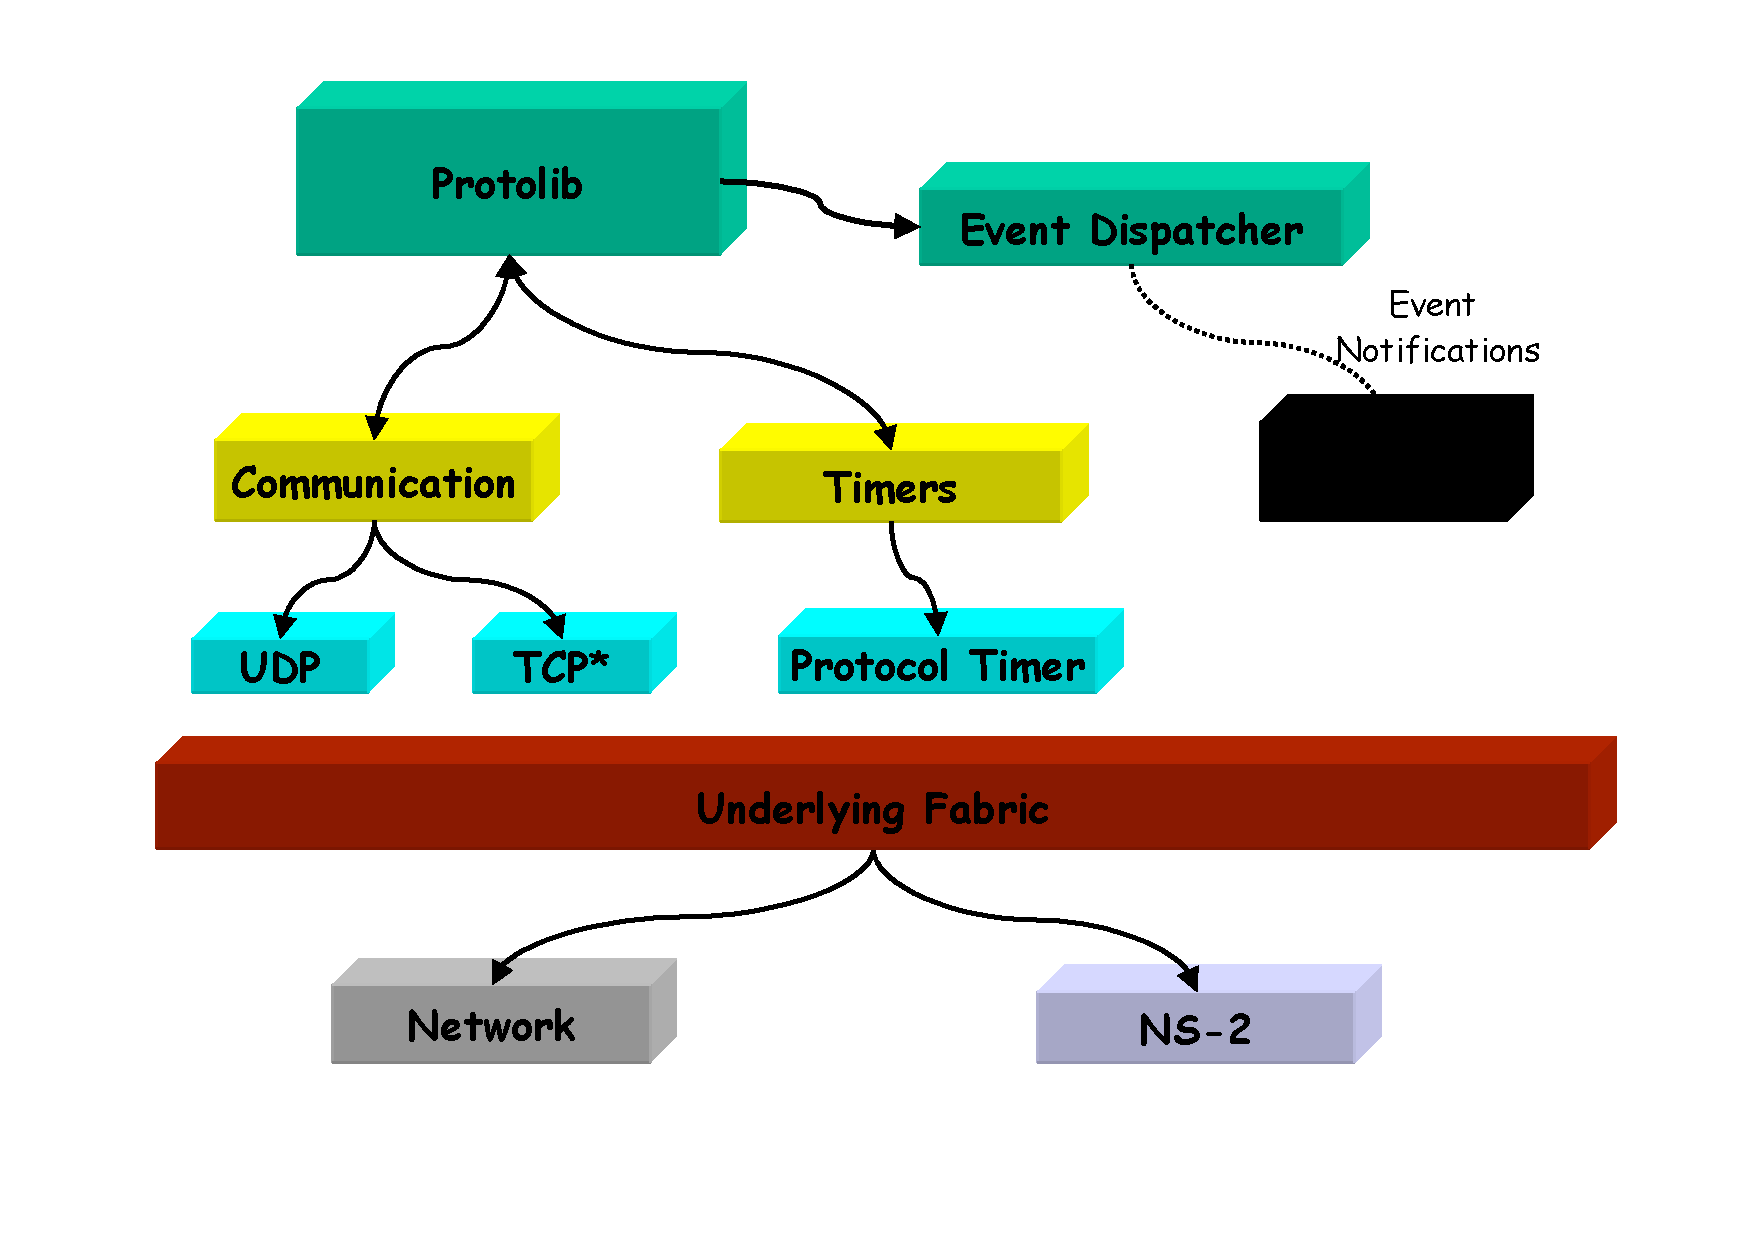
\includegraphics[scale=0.4]{images/protolibOverview}
\caption{An overview of the Protolib toolkit, showing the three distinct 
components, sockets timers and a mechanism for dispatching events.} 
\label{pai:fig:overview}
\end{figure}


A typical usage scenario of Protolib is given in the Fig \ref{pai:fig:demo} . Here, a timer is set up to trigger every 100 milliseconds. Upon a trigger event, a C++ callback is invoked that allows the application developer to integrate an event action. In this example, the application sends a UDP message using Protolib.  This communication mechanism can be achieved using a standard UDP call across a network or between two NS-2 nodes.  When the packet is received by the receiver, another event is generates indicating that data has been received.  This, in turn, calls a routine that allows the application to collect the data from the UDP port and process it in some way. The application interface between the Protolib and the P2P middleware abstracts the reliance on specific networking/timing mechanisms in Protolib to create a generalized pluggable transport mechanism. Within PAI, middleware or indeed applications program to one interface and then choose the environment they want to run within e.g.  Network or NS-2. This is very similar to GATLite but at a far lower level.  PAI also support multiple sockets, timers and corresponding listeners for timeouts or UDP receive data events and establishes a cooperating event dispatching mechanism using multithreading.

\begin{figure}
\centering
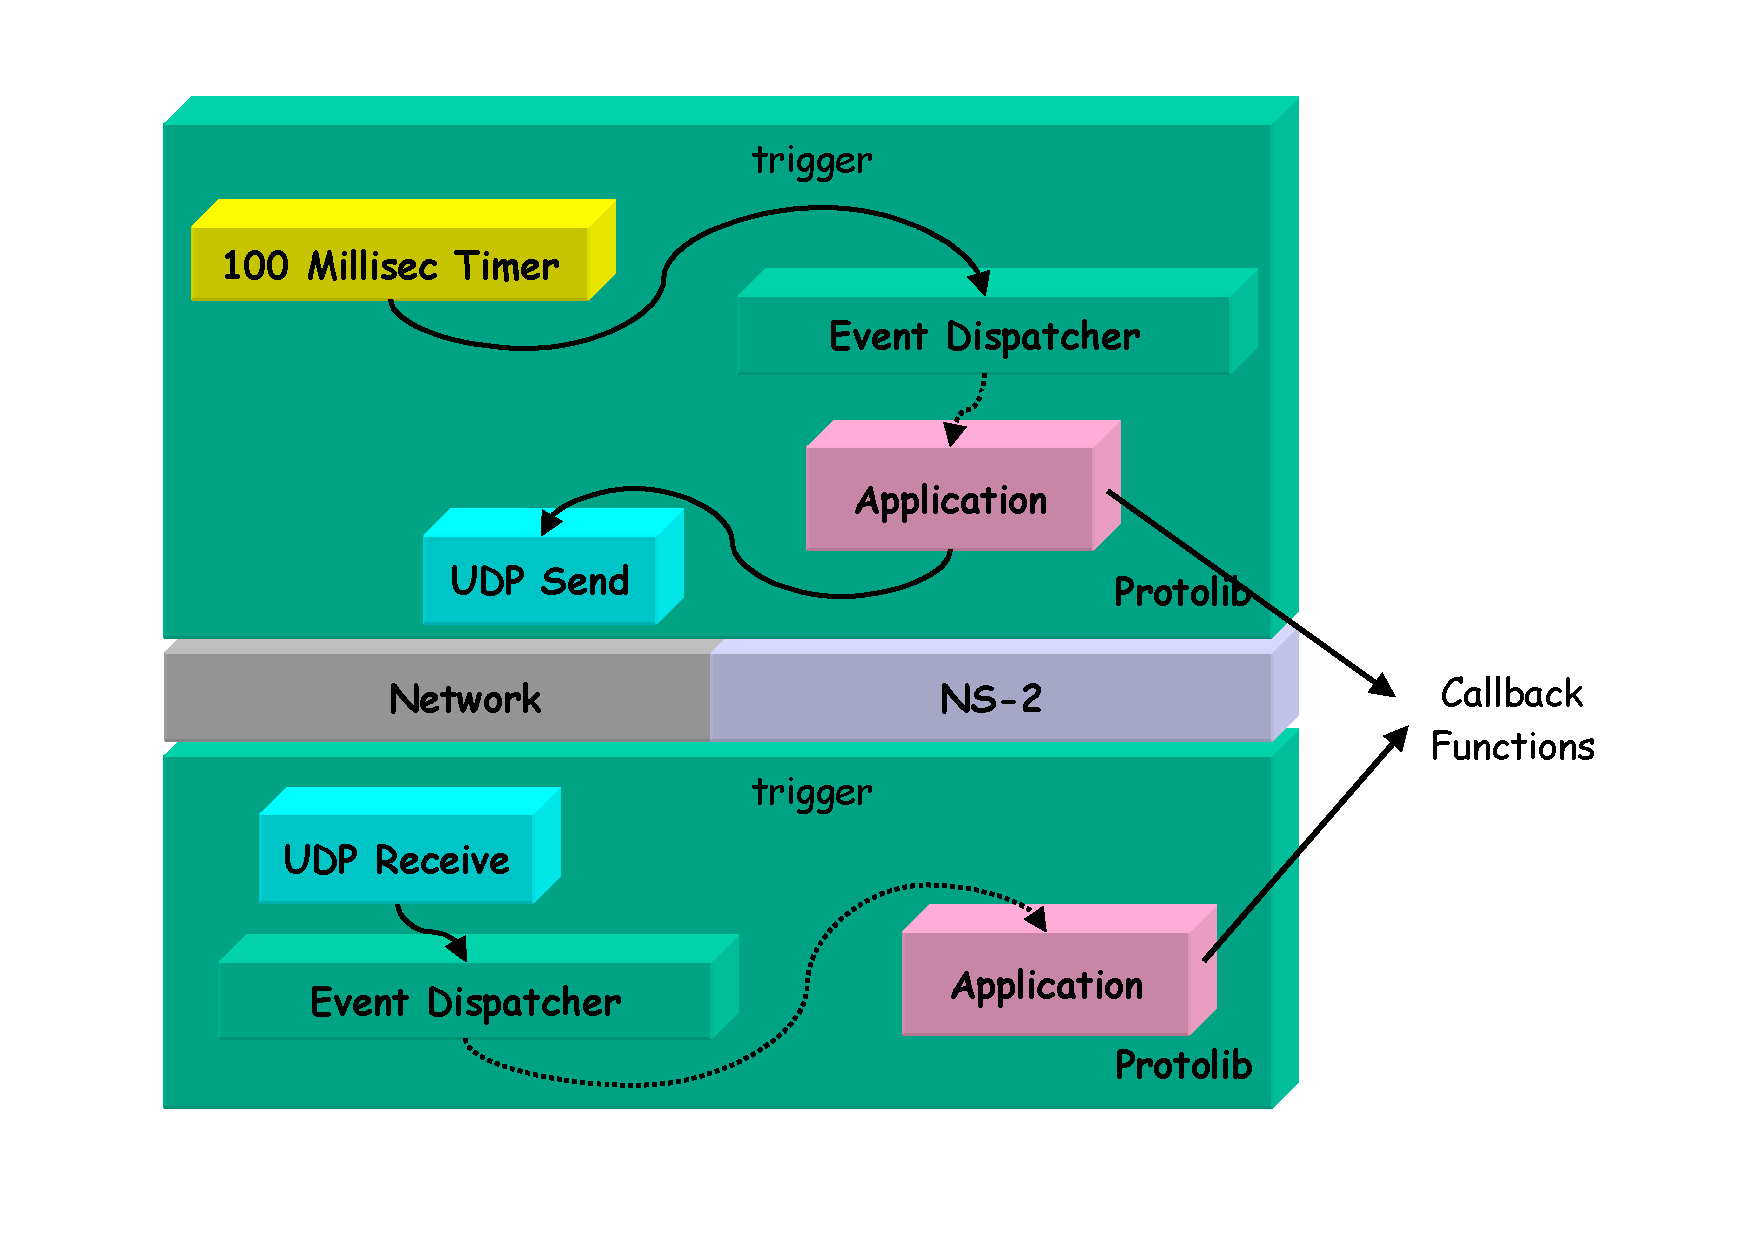
\includegraphics[scale=0.4]{images/protolibDemo}
\caption{An overview of the functionality provided by the ProtoApp
application, which triggers a data send once-per-second.} 
\label{pai:fig:demo}
\end{figure}

\section{Protolib Structure}

The following classes are contained within the Protolib toolkit (taken from the descriptions provide in the release\footnote{Given by Brian Adamson, email: adamson@itd.nrl.navy.mil})

\begin{itemize}
\item \textbf{ProtoAddress:}    Network address container class with support
                 for IPv4, IPv6, and "SIM" address types.  Also
                 includes functions for name/address
                 resolution.

\item \textbf{ProtoSocket:}     Network socket container class that provides
                 consistent interface for use of operating
                 system (or simulation environment) transport
                 sockets. Provides support for asynchronous
                 notification to ProtoSocket::Listeners.  The
                 ProtoSocket class may be used stand-alone, or
                 with other classes described below.  A
                 ProtoSocket may be instantiated as either a
                 UDP or TCP socket.

\item \textbf{ProtoTimer:}      This is a generic timer class which will
                 notify a ProtoTimer::Listener upon timeout.
\item \textbf{ProtoTimerMgr:}   This class manages ProtoTimer instances when
                 they are "activated".  The ProtoDispatcher
                 (below) derives from this to manage
                 ProtoTimers for an application.  (The
                 ProtoSimAgent base class contains a
                 ProtoTimerMgr to similarly manage timers for a
                 simulation instance).

\item \textbf{ProtoTree: }      Flexible implementation of a Patricia tree
                 data structure.  Includes a ProtoTree::Item
                 which may be derived from or used as a
                 container for  whatever data structures and
                 application may require.

\item \textbf{ProtoRouteTable:} Class based on the ProtoTree Patricia tree to
                 store routing table information. Uses the
                 ProtoAddress class to store network routing
                 addresses.  It's a pretty dumbed-down routing
                 table at the moment, but may be enhanced in
                 the future.  Example use of the ProtoTree.

\item \textbf{ProtoRouteMgr:}   Base class for providing  a conistent
                 interface to manage operating system (or
                 other) routing engines.
\item \textbf{ProtoDispatcher:} This class provides a core around which Unix
                 and Win32 applications using Protolib can be
                 implemented.  It's "Run()" method provides a
                 "main loop" which uses the "select()" system
                 call on Unix and the similar
                 "MsgWaitForMultipleObjectsEx()" system call on
                 Win32.  It is planned to eventually provide
                 some built-in support for threading in the
                 future (e.g. the ProtoDispatcher::Run() method
                 might execute in a thread, dispatching events
                 to a parent thread).
\item \textbf{ProtoApp: }       Provides a base class for implementing
                 Protolib-based command-line applications. Note
                 that "ProtoApp" and "ProtoSimAgent" are
                 designed such that subclasses can be derived
                 from either to reuse the same code in either a
                 real-world applications or as an "agent"
                 (entity) within a network simulation
                 environment (e.g. ns-2, OPNET).  A "background"
                 command is included for Win32 to launch the
                 app without a terminal window.

\item \textbf{ProtoSimAgent:}   Base class for simulation agent derivations. 
                 Currently an ns-2 agent base class is derived
                 from this, but it is possible that other
                 simulation environments  (e.g. OPNET, Qualnet)
                 might be supported in a similar fashion.

\item \textbf{NsProtoSimAgent:} Simulation agent base class for creating ns-2
                 instantiations of Protolib-based network
                 protocols and applications.
\item \textbf{ProtoExample:}    Example class which derives either from
                 ProtoApp or NsProtoSimAgent, depending upon
                 compile-time macro definitions.  It provides
                 equivalent functionality in either the
                 simulation environment or as a real-world
                 command-line application.  It demonstrates the
                 use/operation of ProtoSocket based UDP
                 transmission/reception, a ProtoTimer, and an
                 example ProtoSocket-based TCP client-server
                 exchange.   (NOTE: TCP operation is not yet
                 supported in the simulation environment.  This
                 will completed in coming months.  I plan to
                 extend ns-2 TCP agents to support actual
                 transfer of user data to support this.)
\item \textbf{Other:} The Protolib code also includes some simple, general purpose debugging routines which can output to "stderr" or optionally log to a specified file. 
See "protoDebug.h" for details. 

\end{itemize}

\section{Conclusion}


In this chapter, a brief overview of the Protolib toolkit was given.  We gave an overview of its structure and the types of operations it is designed to support (e.g. UDP/TCP communication, timers and event dispatching) and illustrated this through the use of a simple but typical usage scenario. We then gave an overview of the key classes that make up the toolkit. 

Protolib is an evolving toolkit.  As PAI has been integrated on top of Protolib, it has been updated in order to support the functionality required by \agentj~and its applications. PAI, described in the next chapter, focuses on providing the interfaces necessary for Java applications and middleware to use Protolib in a number of different contexts.


\chapter{The PAI Interface}
\label{pai}

The Protolib Application Interface (PAI) provides a layer that allows Protolib to be used Java applications. Specifically, it provides a generic interface to timers, sockets and dispatchers and then employs the use of the \emph{factory method design pattern} in order to instantiate the required set of objects e.g. UDP sockets, TCP NS2 sockets, realtime timers, NS2 timers, NS2 event dispatchers etc.  

The resulting PAI interface looks very similar to a Java interface. Where ever 
possibly, we have used the Java conventions for interfacing with the underlying objects. For example, instead of providing callback functions for a timer, we allow a user to attach multiple listeners to a timer in order to get notified when an event occurs.  The resulting interface therefore is very simple and very Java friendly.  

In this chapter, we give a brief overview of PAI and provide some programming examples of its use. We then show how PAI can be used within NS2 by providing a PAI NS2 agent for integrating with Protolib.

\section{Overview of PAI}

\begin{figure}
\centering
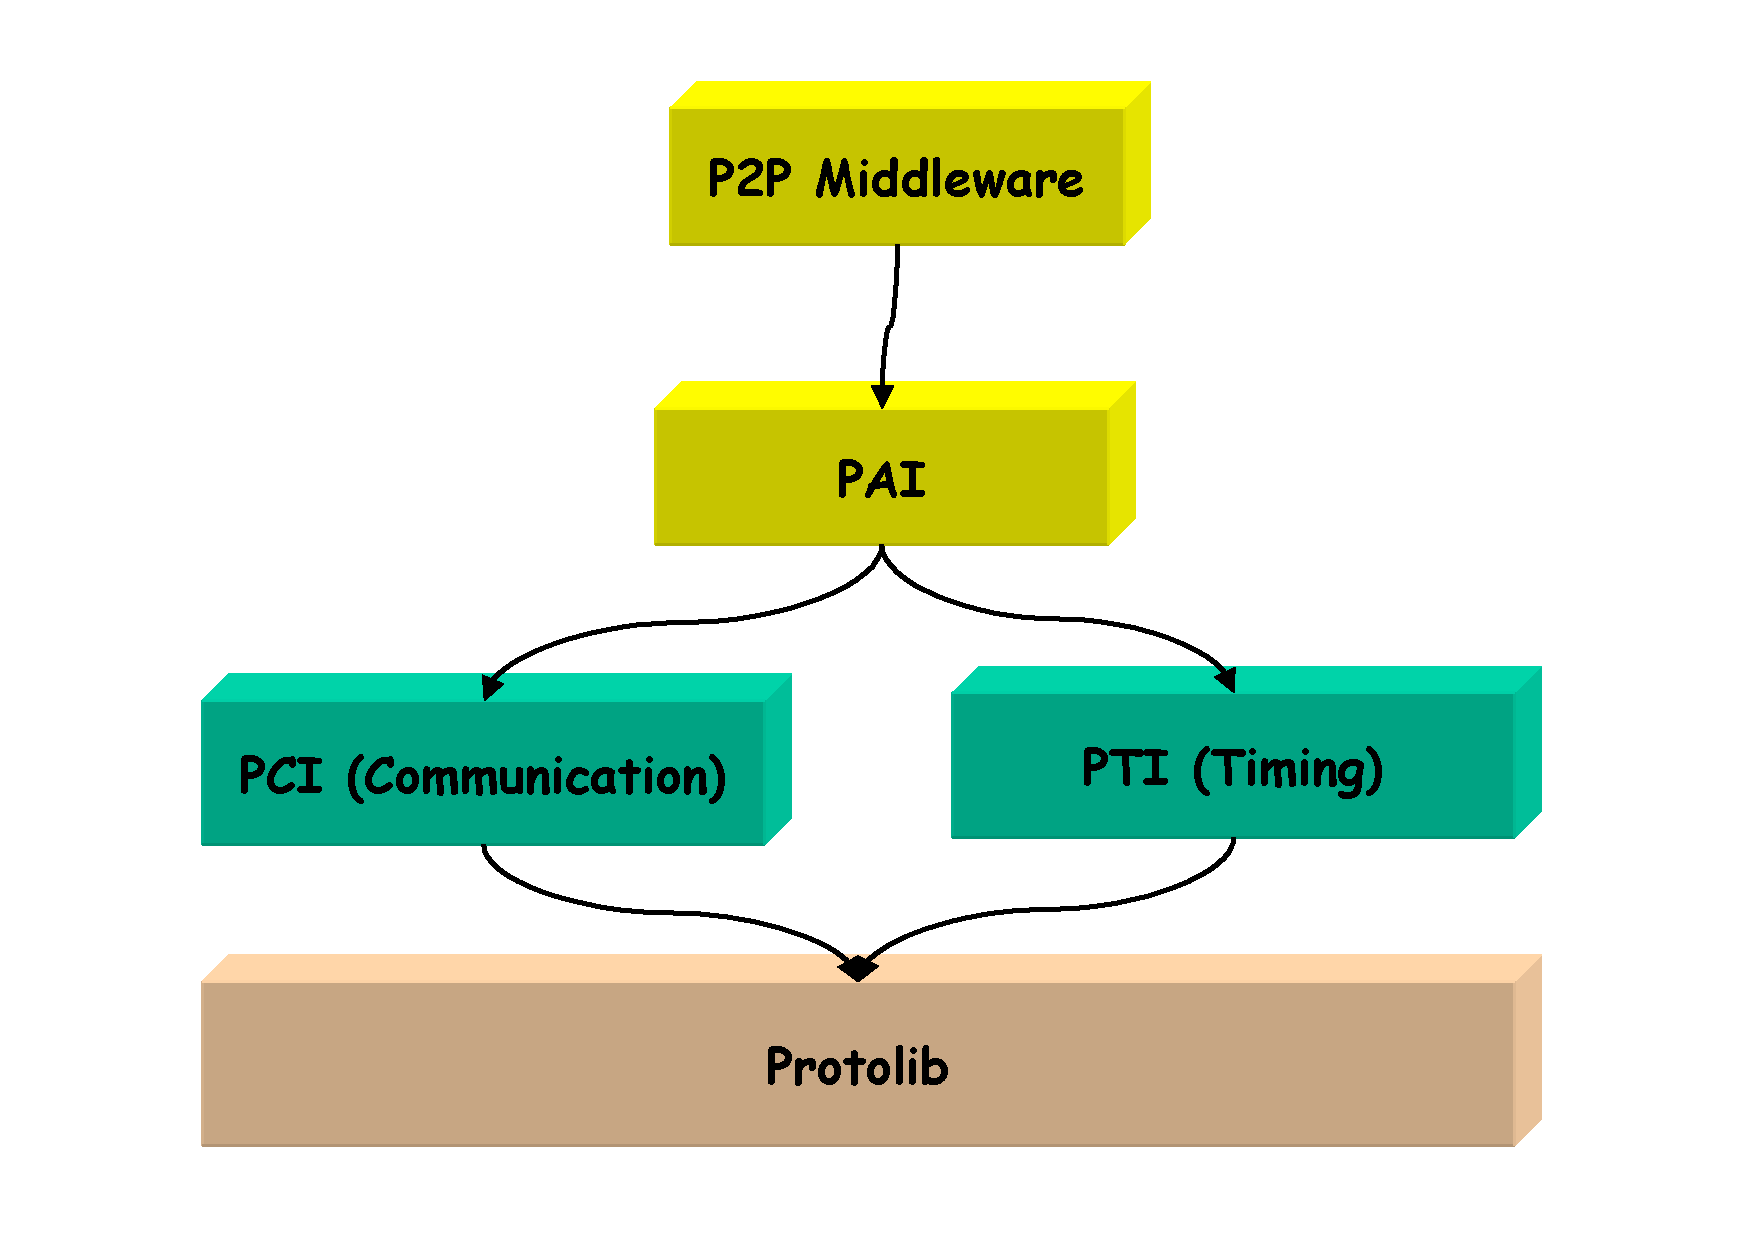
\includegraphics[scale=0.4]{images/paiOverview}
\caption{An overview of the PAI interface, showing the two sections to the
underlying Protolib sockets and timers.} 
\label{pai:fig:overview}
\end{figure}

\begin{figure}
\centering
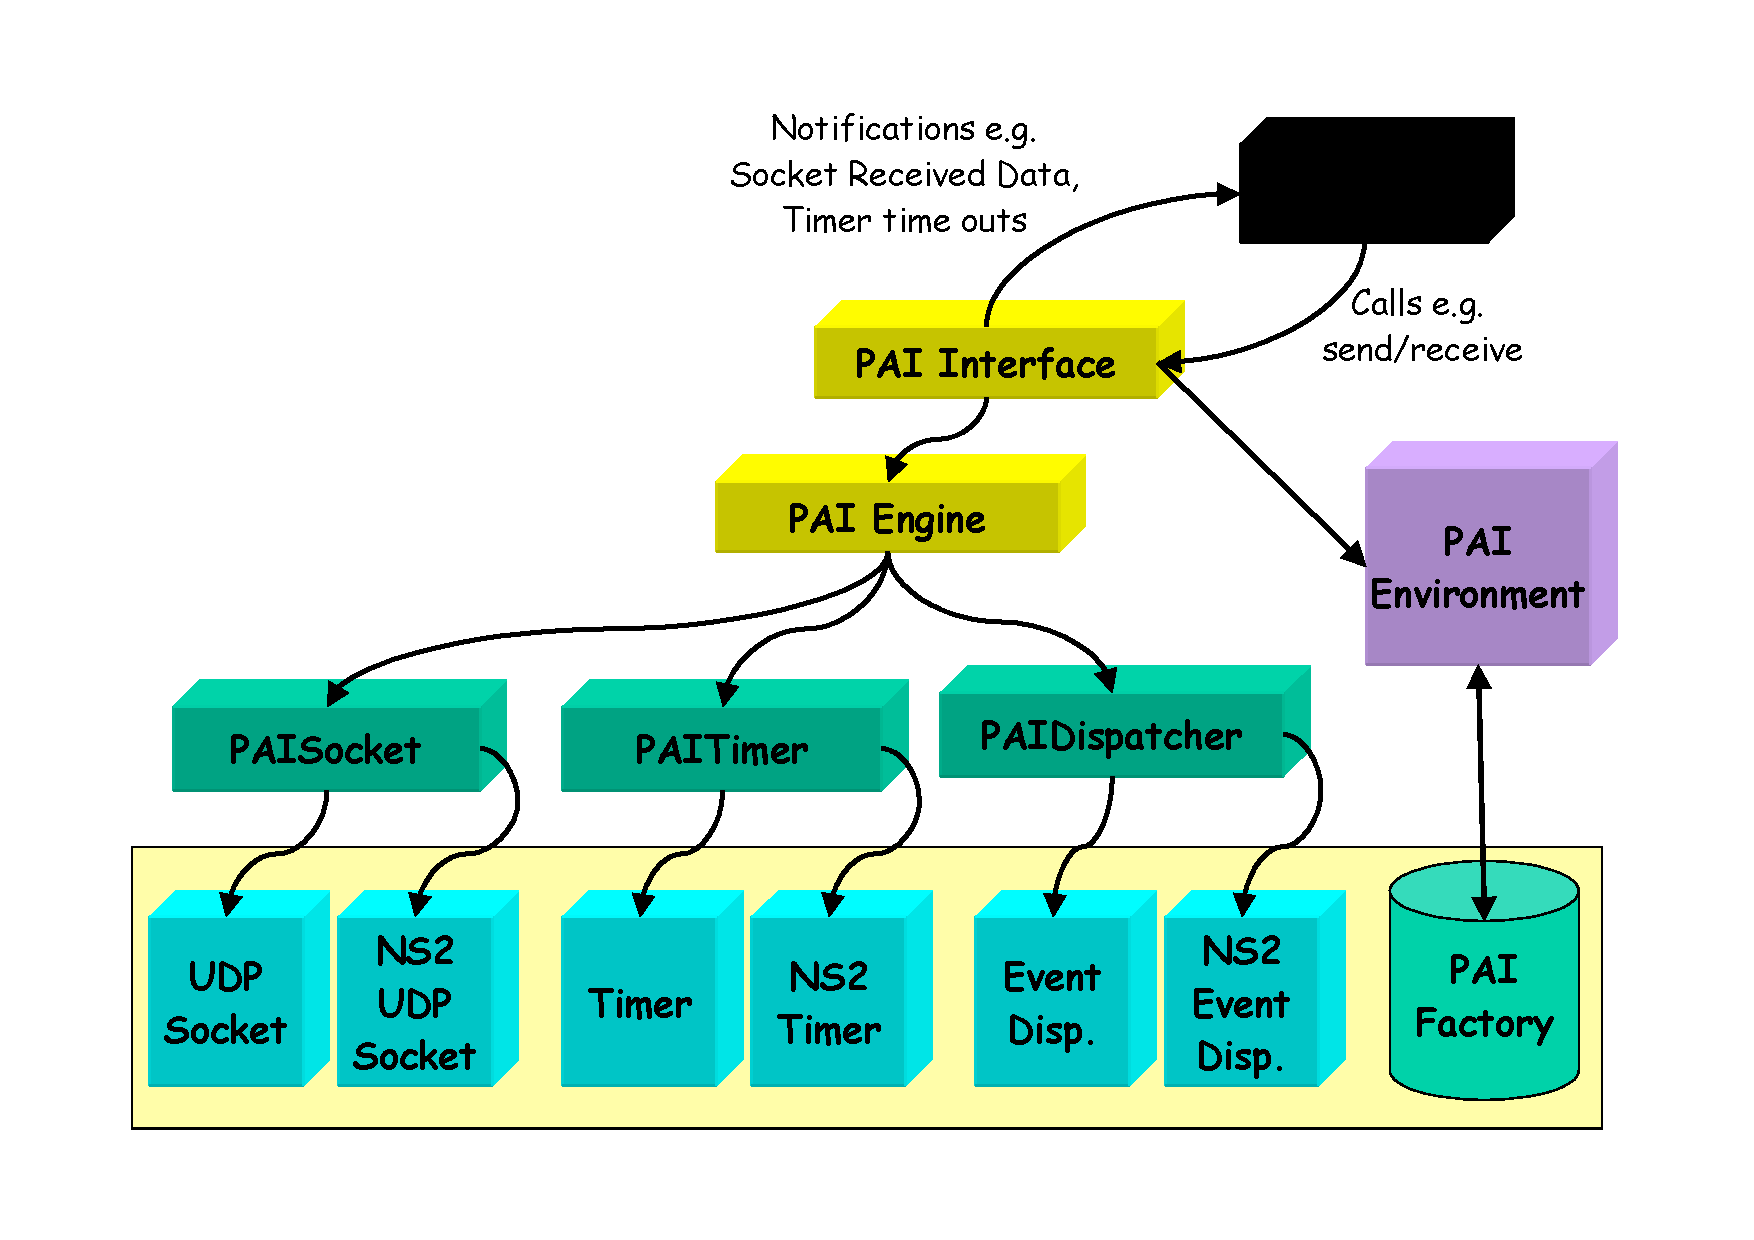
\includegraphics[scale=0.4]{images/paiFactory}
\caption{The PAI interface uses the Factory design pattern to create
a common high level interface to whatever sockets or underlying timers
the programmer is using.} 
\label{pai:fig:factory}
\end{figure}


\section{Programming PAI}



\begin{figure}
\centering
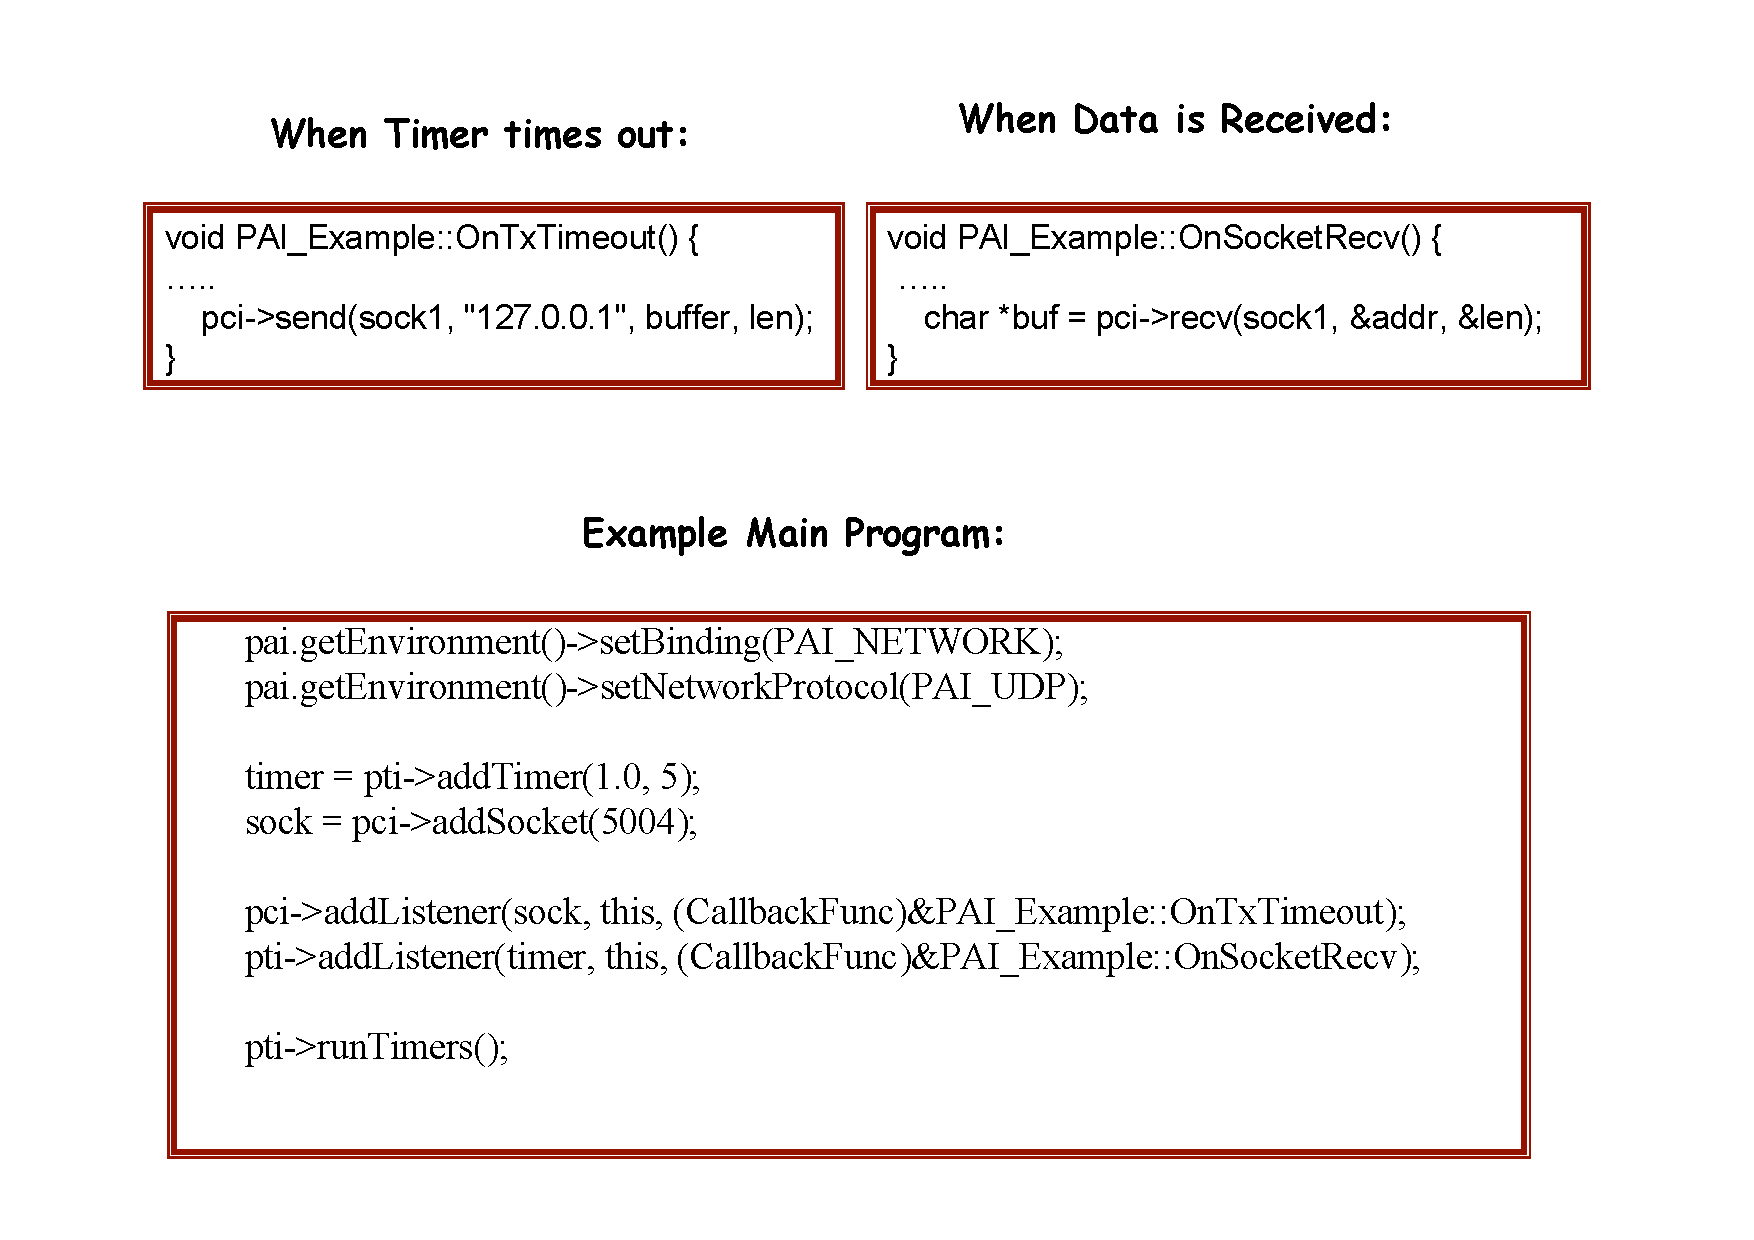
\includegraphics[scale=0.4]{images/paiExample}
\caption{An PAI code example, showing how you would implemented the 
standard Protolib demonstration, which sets of a 1 second timer and sends
data between two nodes.} 
\label{pai:fig:example}
\end{figure}


\section{Using PAI within NS2: The C++ Side}
\label{jni:nodeint}

\index{NS2}

The Java PAI interface described in the last Chapter can be used 
directly by C++ applications within NS2.  This chapters discusses
the C++ agent classes that have been written for \agentj and
how these can be used with PAI to pass data between NB2 nodes
and to set off timers.

\section{Ns2 Agents}

There are typically two main components within an NS2 scenario:

\begin{enumerate}
\item \textbf{C++ Agent:} This is used to represent the C++ behaviour
within Ns2.  Examples of agents could include transport protocols e.g.
UDP agent, TCP agent etc.  Agents can also be use to implement 
applications (using Protolib) or to broker them. 
\item \textbf{TCL Script:} This sepcifies which NS2 C++ agents will be used
and also to paint the scenario of the simulation you wish to perform
within the simulation environment.
\end{enumerate}

\begin{figure}
\centering
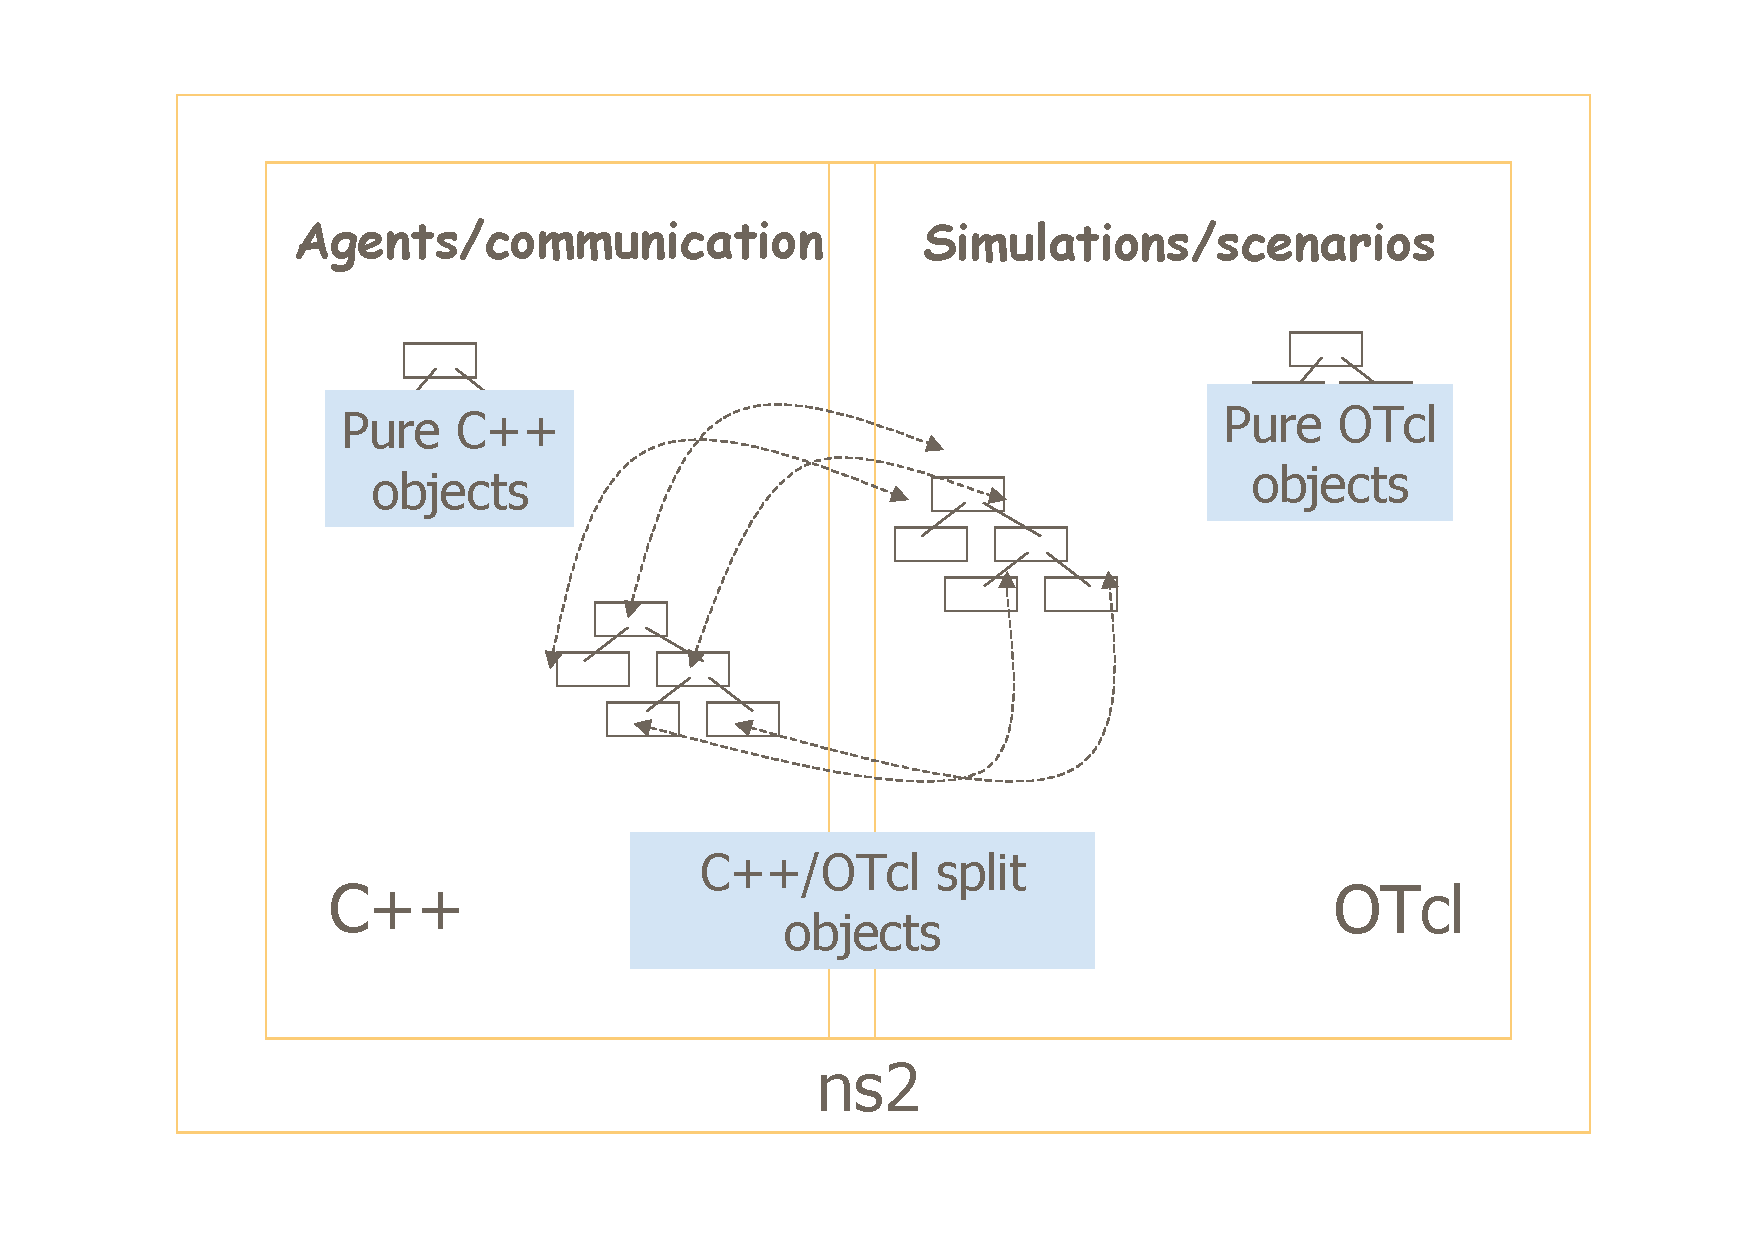
\includegraphics[scale=0.4]{images/paiAgentsTCLandC}
\caption{An overview of how TCL interacts with C++ agents within Ns2 } 
\label{paiagent:fig:paiAgentsTCLandC}
\end{figure}

Figure \ref{paiagent:fig:paiAgentsTCLandC} illustrates how these two
components interacts within NS2.  The TCL script sets up the environment,
e.g., the communication links, the underlying network core, and specifies
which agents are going to be used  within the simulation. An example
script is given below, which simply creates a BasicAgent class and
invokes a 'hello' command on that agent.

\footnotesize
\begin{verbatim}
set ns_ [new Simulator]

# Create two nodes
set n1 [$ns_ node]
set n2 [$ns_ node]

# Put a link between them
$ns_ duplex-link $n1 $n2 64kb 100ms DropTail
$ns_ queue-limit $n1 $n2 100
$ns_ duplex-link-op $n1 $n2 queuePos 0.5
$ns_ duplex-link-op $n1 $n2 orient right

set p1 [new Agent/BasicAgent]
$ns_ attach-agent $n1 $p1

puts "Starting simulation ..."

$ns_ at 0.0 "$p2 hello"
$ns_ at 1.0 "finish $ns_"

proc finish {ns_} {
$ns_ halt
delete $ns_
}

$ns_ run
\end{verbatim}
\normalsize

As you can see from the script, two Ns2 nodes are created and
a network link is specified between them. We then create
a custom Agent (called Basic Agent) and invoke a simple command on
that agent.   We are interested here in how such commands get 
passed to the agents.  For specifics and a compendium of 
example scripts and agents can be found in the Ns-2 manual
at the web site \cite{ns2}.

TCL scripts communicate with the C++ agents that they create by
passing them commands.  These commands get passes to a
standardized method within the C++ Agent, called:

\footnotesize
\begin{verbatim}
int PAIAgent::command(int argc, const char*const* argv) {
\end{verbatim}
\normalsize

\noindent where, conventionally (as in main()), the arguments provide the following information:

\begin{itemize}
\item \textbf{argc:} specifies the number of strings representing the command
and arguments which are being sent (i.e. args 1 contains the command and 
2 onwards specifies the arguments for the command).    
\item \textbf{argv:} These contain the actual strings representing the command
and its arguments.
\end{itemize}

Therefore, a command, such as:

\footnotesize
\begin{verbatim}
$ns_ at 0.0 "$p2 hello"
\end{verbatim}
\normalsize

\noindent would be caught by the following command method implementation:


\footnotesize
\begin{verbatim}
int PAIAgent::command(int argc, const char*const* argv) {

    if (2 == argc) {
        if (!strcmp(argv[1], "hello")) {
		cout << "BasicAgent: received a hello! " << endl;
                return TCL_OK;			
                }
        // else if  ... 
        }

    // invoke the command from the next object up in the Agent class hierarchy
    
    return NsProtoAgent::command(argc, argv);
}	
\end{verbatim}
\normalsize

The PAI agents, described in the next section build upon this basic 
framework and Protolib to allow real applications to be run within the
NS2 simulation environment. 
  
\section{PAI Agents and Protolib}

\begin{figure}
\centering
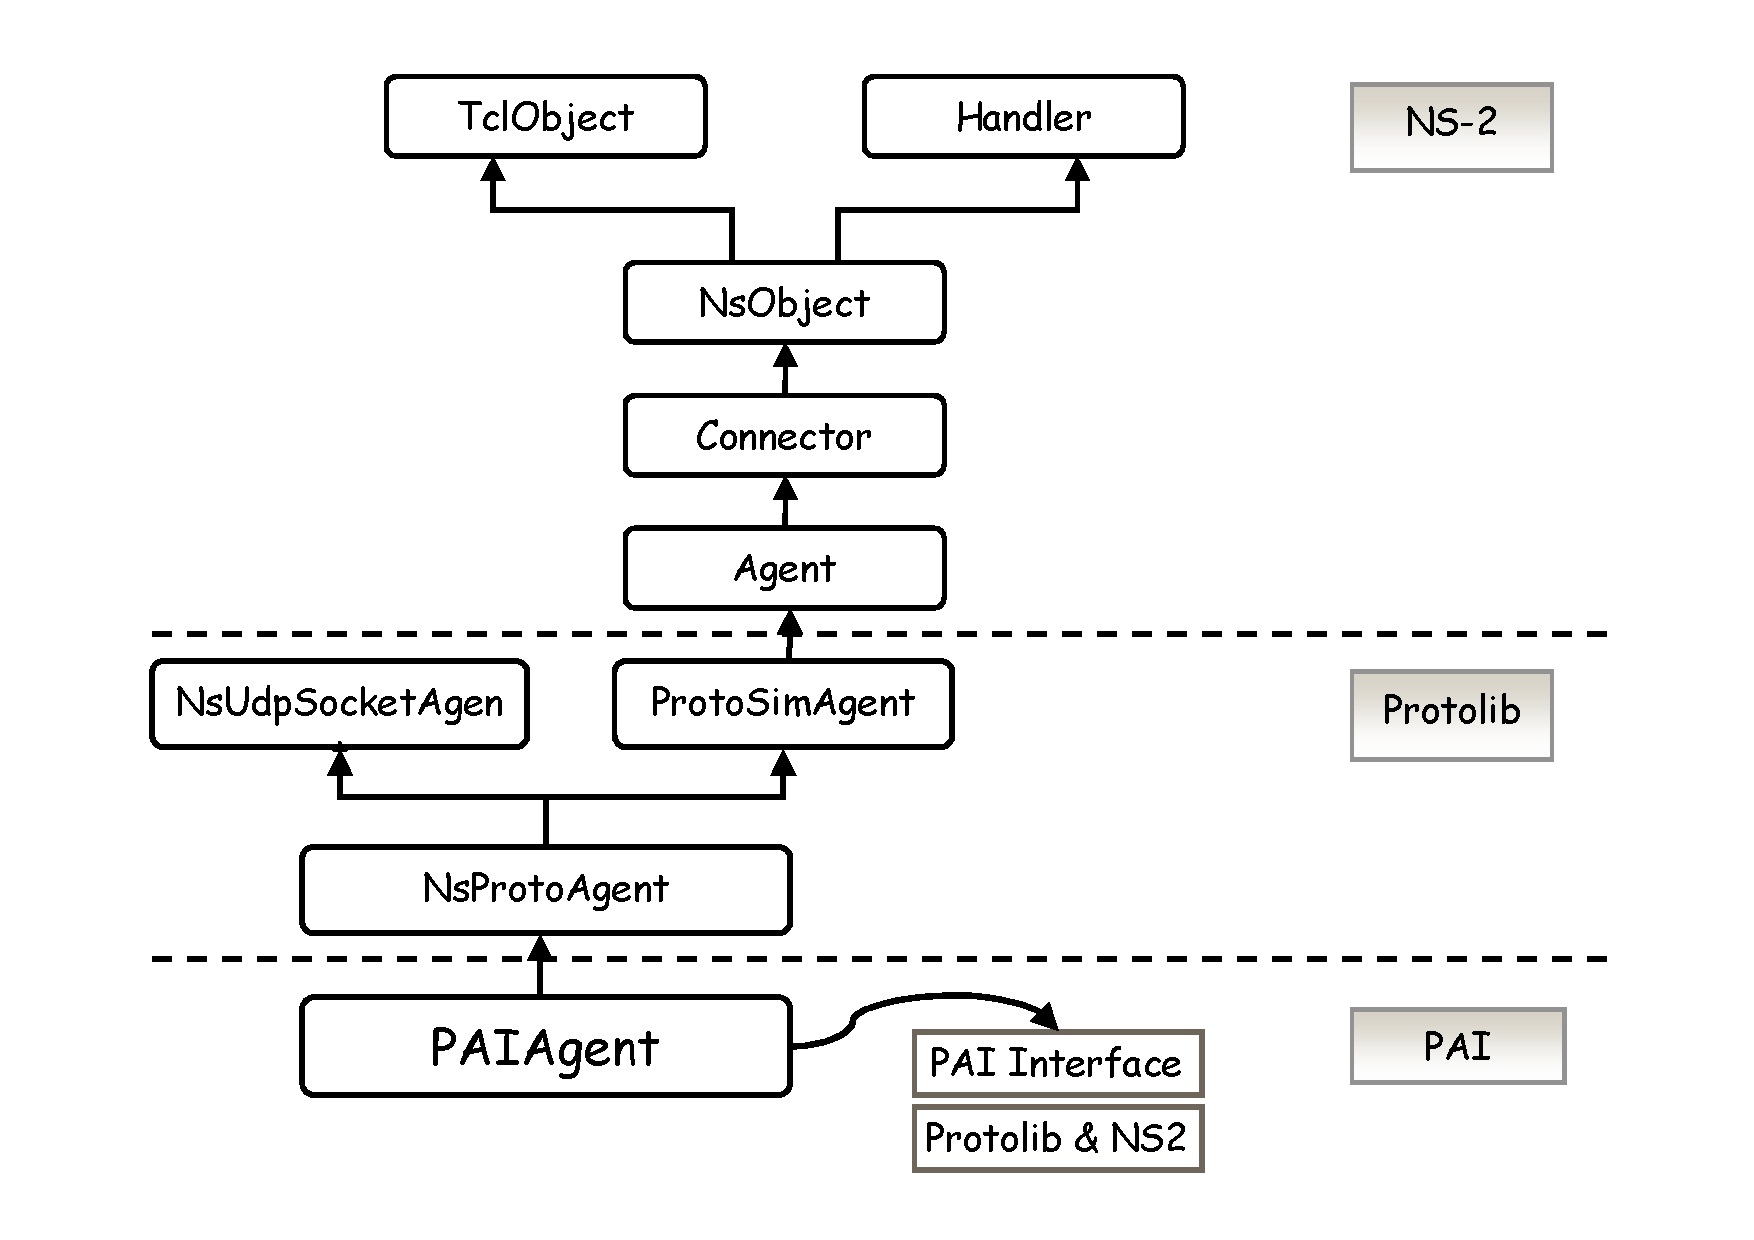
\includegraphics[scale=0.4]{images/paiAgentsClassHeirarch}
\caption{The Class structure of the NS2, Protolib and PAI classes to form the 
PAI agent hierarchy within NS2} 
\label{jni:fig:paiAgentsClassHeirarch}
\end{figure}

\section{Conclusion}


\chapter{\agentj: Java Agents in NS2}
\label{agentj}

In this chapter, we present the design and implementation of the \agentj~
framework and show the various levels at which \agentj~interacts with other
software packages and implements its functionality. In the previous two 
chapters, Protolib and the PAI interface were described which form the 
building blocks for \agentj. This chapter shows how these have been integrated 
through extensive use of the java Java Native Interface (JNI). 

The first section provides an overview of the cooperating software 
components and the following section describes the core 
C++ and Java classes which have been used to implement these. Then,
for completeness, we present the Java version of the PAI interface, which
is at the core of this integration. Finally, we give a summary this integration by
providing a complete overview of the software component interactions and
the corresponding classes which implement the core behaviour of the system.  

Although, the understanding of the details of this chapter is not absolutely necessary 
for \agentj~users, it is highly recommended reading, as the details given here will
give a broad understanding of the \agentj~system and therefore, help a potential
user in understanding what s/he can and cannot do. 
 

\section{\agentj~Software Overview}
\label{agentj:nodeint}

Using \agentj, each C++ NS2 agent can (optionally) attach a Java agent. A 
Java Ns2 agent is a Java program that can be accessed through the 
standard \agentj~ interface, which allows it to receive commands in the 
same ways as C++ NS2 agents do. Thus, specifically, an \agentj~node is:

\emph{
\begin{quote}
A Java object that implements the \emph{AgentJObject} 
interface
\end{quote}
}

\vspace{0.2in}


\agentj~nodes can use any 3rd party Java application in order to
implement the behaviour they require. Further \agentj~nodes can
use the \agentj's PAI binding to access standard communication and 
timing classes in order to schedule events and discover and
communicate with other \agentj~nodes. In this fashion, complete
Java simulations can be built up using these simple primitives. 


For a Java application top become a \agentj~node, it only needs to 
implement a simple Java interface and so the overhead of converting a
Java applications into the \agentj~framework is minimal i.e. far easier 
that writing an Applet, for integration into another type of environment 
e.g. a Web browser.  However, for such \agentj~nodes to 
communicate with other nodes, they will need to interface with 
\agentj's re-implementations of the normal Java classes they would 
use. This normally involves replacing all occurances of 
\emph{java.net.} with \emph{pai.net.}.  We used precisely this procedure 
to integrate the  P2PS middleware, discussed in \cite{p2psx}.  

\index{P2PS}
\index{Applet}

In this section, we describe how the \agentj~framework 
has been integrated using JNI and the core C++ Protolib and PAI 
toolkits and Java classes. 

\index{PAI}
\index{Protolib}

\subsection{Creating \agentj~Nodes}
\label{agentj:creating}

\begin{figure}
\centering
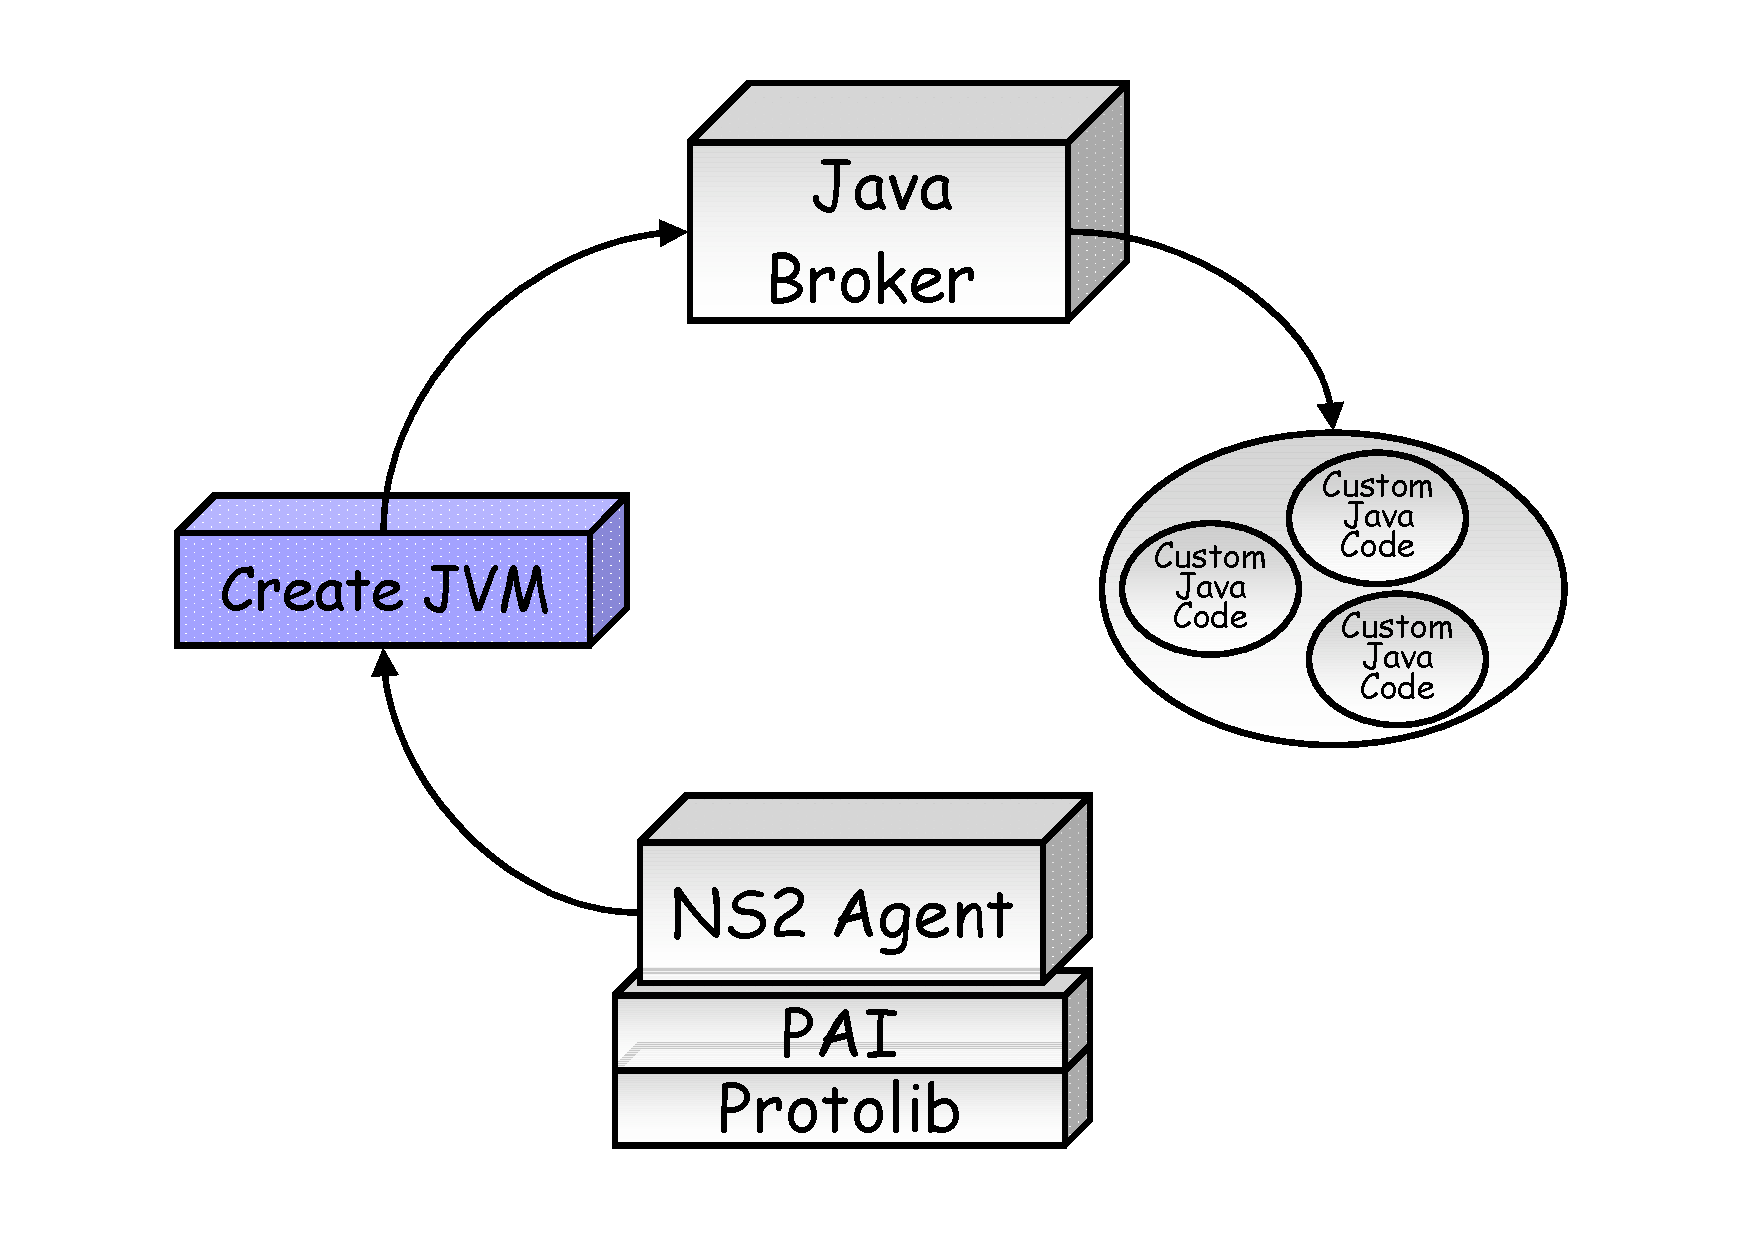
\includegraphics[scale=0.3]{images/agentjOverview}
\caption{\agentj~can attach any conforming Java object to an NS2 agent.} 
\label{agentj:fig:javaOverview}
\end{figure}

Figure \ref{agentj:fig:javaOverview} gives an overview of the software
architecture employed by \agentj~and shows how Java fits into
this picture.  Each NS2 \emph{agent} can attach a Java 
object (i.e. Java agent) by accessing a Java Virtual machine (JVM) 
and by requesting that an association be made within the Java domain
between the desired Java object and itself.  This request 
results in a Java Hashtable being populated with an item pair; with the 
C++ agent pointer representing the key and \agentj~Java object 
representing the object.   

\index{NS2}
\index{JNI}
\index{Java}
\index{JVM}

There could potentially be thousands of NS2 nodes and each one 
might want to instantiate and use a Java object.  Therefore serious 
scalability issues can be encountered if this interaction is not 
slimline enough. In \agentj, the C++ JVM helper class (C2JBroker) therefore
only allows \textbf{ONE} JVM to be  created no matter how many 
nodes exist in the simulations.  This JVM instantiates a singleton
the \emph{JavaBroker} class, which creates and manages the external 
Java objects. \emph{JavaBroker} contains functionality that can 
dynamically create a Java object from a textual representation of its
name (e.g. pai.examples.NS2.SimpleCommand). 

Once created such objects are added to a local Hashtable, which associates 
an NS2 agent's \emph{ID} with the associated object that has been created for this 
interaction.  The NS2 agent's \emph{ID} is actually its C++ pointer, which 
is reused later within the JNI binding (see below). Therefore, 
each NS2 node only instantiates the Java class it needs
rather than any other wrapping classes. This implementation therefore 
maps one-to-one between the C++ NS2 agent and its corresponding 
Java object and therefore keeps the memory allocation to an absolute 
minimum; that is, we do not create thousands of 
\emph{JavaBroker} objects, rather, we create one and have this act as
a central locator for all Java objects. 

The Java Hashtable is a static Class member (of JavaBroker.java, 
see section \ref{agentj:classes}) and therefore only one Hashtable exists for 
all Java agents.  When a node wishes to send a message to its attached 
Java object, it must first locate this object by searching this Hashtable using
the pointer to the C++ agent.  Once it has obtained a reference to the 
Java agent, it can forward the command to the object.  This searching
overhead is necessary for the issues discussed above in addressing
scalability. 

\subsection{Inter-\agentj~Communication}

Once an \agentj~node has been created and attached to its C++ 
counterpart, it can then use the supported \agentj~communication
and timing protocols in order to schedule events and 
communicate with other \agentj~nodes. \agentj~nodes do this
by using \textbf{standard Java interfaces} which have been 
re-implemented in order to bind to the simulation world within 
NS2. These implementations include:

\begin{itemize}
\item \textbf{UDP Transport:} DatagramSocket and Multicast Socket have been 
rebound to PAI and Protolib to work within NS2.
\item \textbf{TCP Transport:} under construction....
\item \textbf{Inet Support:} a number of the InetAddress methods have been
implemented to work within the NS2 context.
\item \textbf{Timing Libraries:} simple interfaces to timing functions have been 
implemented so that non realtime events (i.e. NS timing events) can be triggered 
at specific intervals during the simulation.
\end{itemize}

This functionality has been implemented by re-implementing the standard Java
interfaces to the networked Java counterparts of these functions. Therefore, in
order to use these within your Java program for example, you simply need to 
import the \emph{pai.net} versions of DatagramSocket and MulticastSocket
rather than the \emph{java.io} versions.


Figure \ref{agentj:fig:javaFullOverview} gives an overview of the lower layers
of this integration and provides a complete picture of how \agentj~uses Java 
within its implementation.  Here, the \agentj~nodes interface through the
Java PAI libraries by using a JNI binding to the C++ PAI and underlying 
Protolib toolkits. It is this software stack that describes the full integration.  
The standard Java interfaces described above merely provide convenient 
access to these libraries.

\begin{figure}
\centering
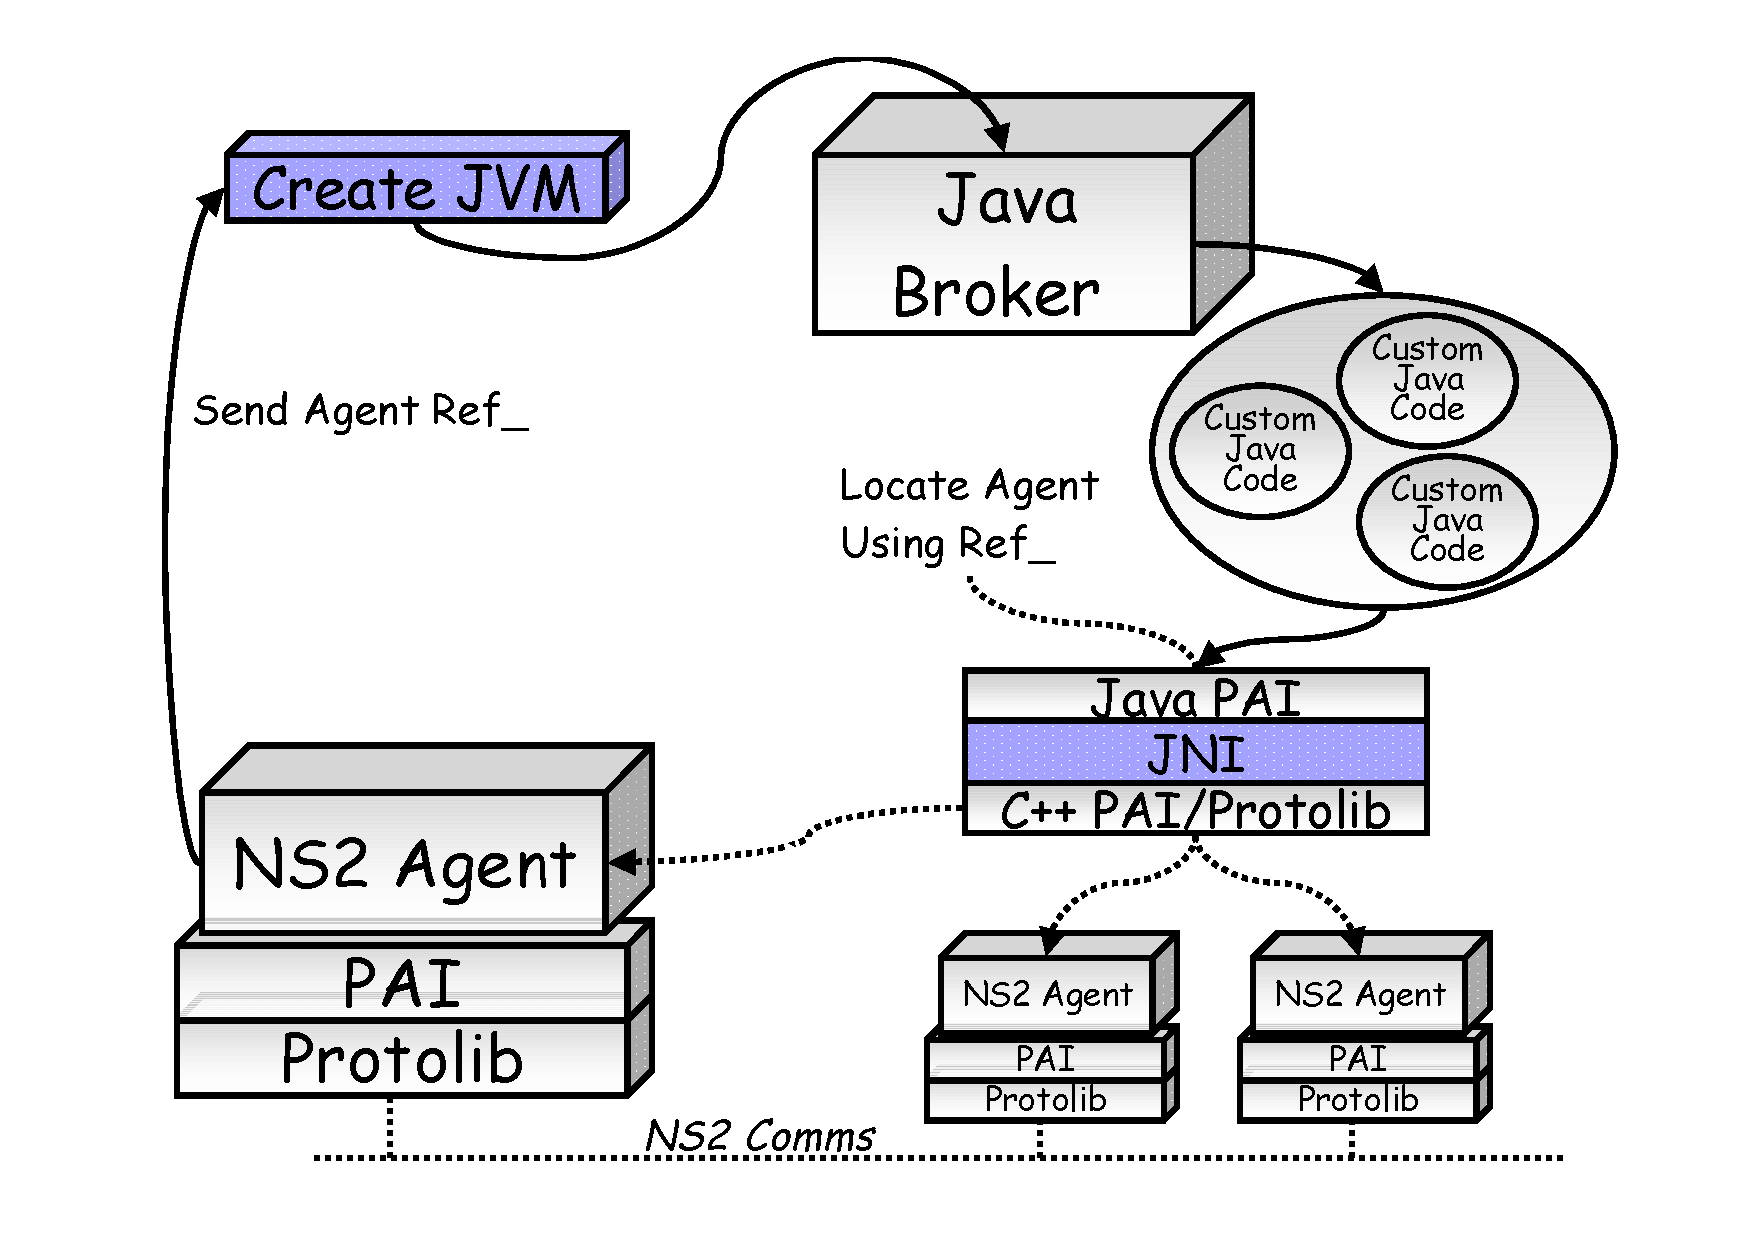
\includegraphics[scale=0.40]{images/agentjFullOverview}
\caption{An overview of the \agentj~software interaction between 
NS2, JNI, PAI and Protolib.} 
\label{agentj:fig:javaFullOverview}
\end{figure}

Therefore, an \agentj~node interacts with other \agentj~nodes 
by binding the standard Java interfaces to the PAI 
socket and timing classes within the JNI implementation, as 
indicated here. This integration allows \agentj~nodes to issue 
commands to send data between NS2 nodes and to set up callbacks
for timing events within NS2. 

For this implementation, a JNI interface is provided 
between the Java PAI interface and the corresponding C++ PAI 
interface that contains the necessary underlying 
functionality. Within this implementation, the \agentj~node's 
\emph{ID} is used along within the JNI binding to the 
PAI interface in order to re-associate the Java object within its 
C++ Ns2 agent when we return back to the C++ context.
In effect, what we are doing here is creating a JVM from C++,
then we are using JNI to re-enter C++. 

However, when we do 
this, JNI has no context and therefore we cannot use static
methods to obtain pointers to parts of the NS2 system. Therefore,
we have to transport these pointers manually through the JVM
so we can re-establish our context when we are back in the
C++ world. Specifically, the \agentj~node needs to be able to 
reference its corresponding C++ NS2 agent so it can invoke
the calls in the appropriate way. Otherwise, how would Protolib
know which node to send the data from?

\section{\agentj~Implementation}
\label{agentj:classes}

This section gives an overview of the classes used to implement
\agentj and describes the key classes that integrate the 
various components together.  There are many underlying 
classes which are not described here but this section
provides a good starting point for those interested in learning 
more about the integration.
 
\agentj~is made up of a collection of C++ and Java classes.  There
are many more C++ classes than Java as the majority of the
implementation is involved in binding between Protolib and
higher level implementations and Java interfaces. For example,
there are many housekeeping classes which provide lookup
tables for mapping between C++ callbacks and Java Listener 
interfaces and vice versa.  

Here, we provide descriptions for the key glue classes that tie the
various parts of the system together between the C++ Java 
classes. The underlying C++ code for PAI and the specifics
of these implementations are out of the scope of this chapter.  

\subsection{Organization of \agentj~Classes}

The \agentj~directorty tree is organized as if it was a Java application.  Therefore,
within this \agentj~directory, there is a classes directory (where all classes 
live), a lib directory (for JAR files plus shared libraries), a doc directory 
(containing this manual) and a src directory (for source files), amongst 
others. 

The src directory also is organized as if it was a Java application also (for the
Java parts AND the C++ parts).  I apologise in advance for this for those
C++ developers who follow different standards but I write C++ programs
as if they were Java and organize them as such! I believe however, that 
the overall structure is organized sensibly and due the the nature of this 
integration it is far easier to maintain a coherency between the Java and
C++ classes. 

\begin{figure}
\centering
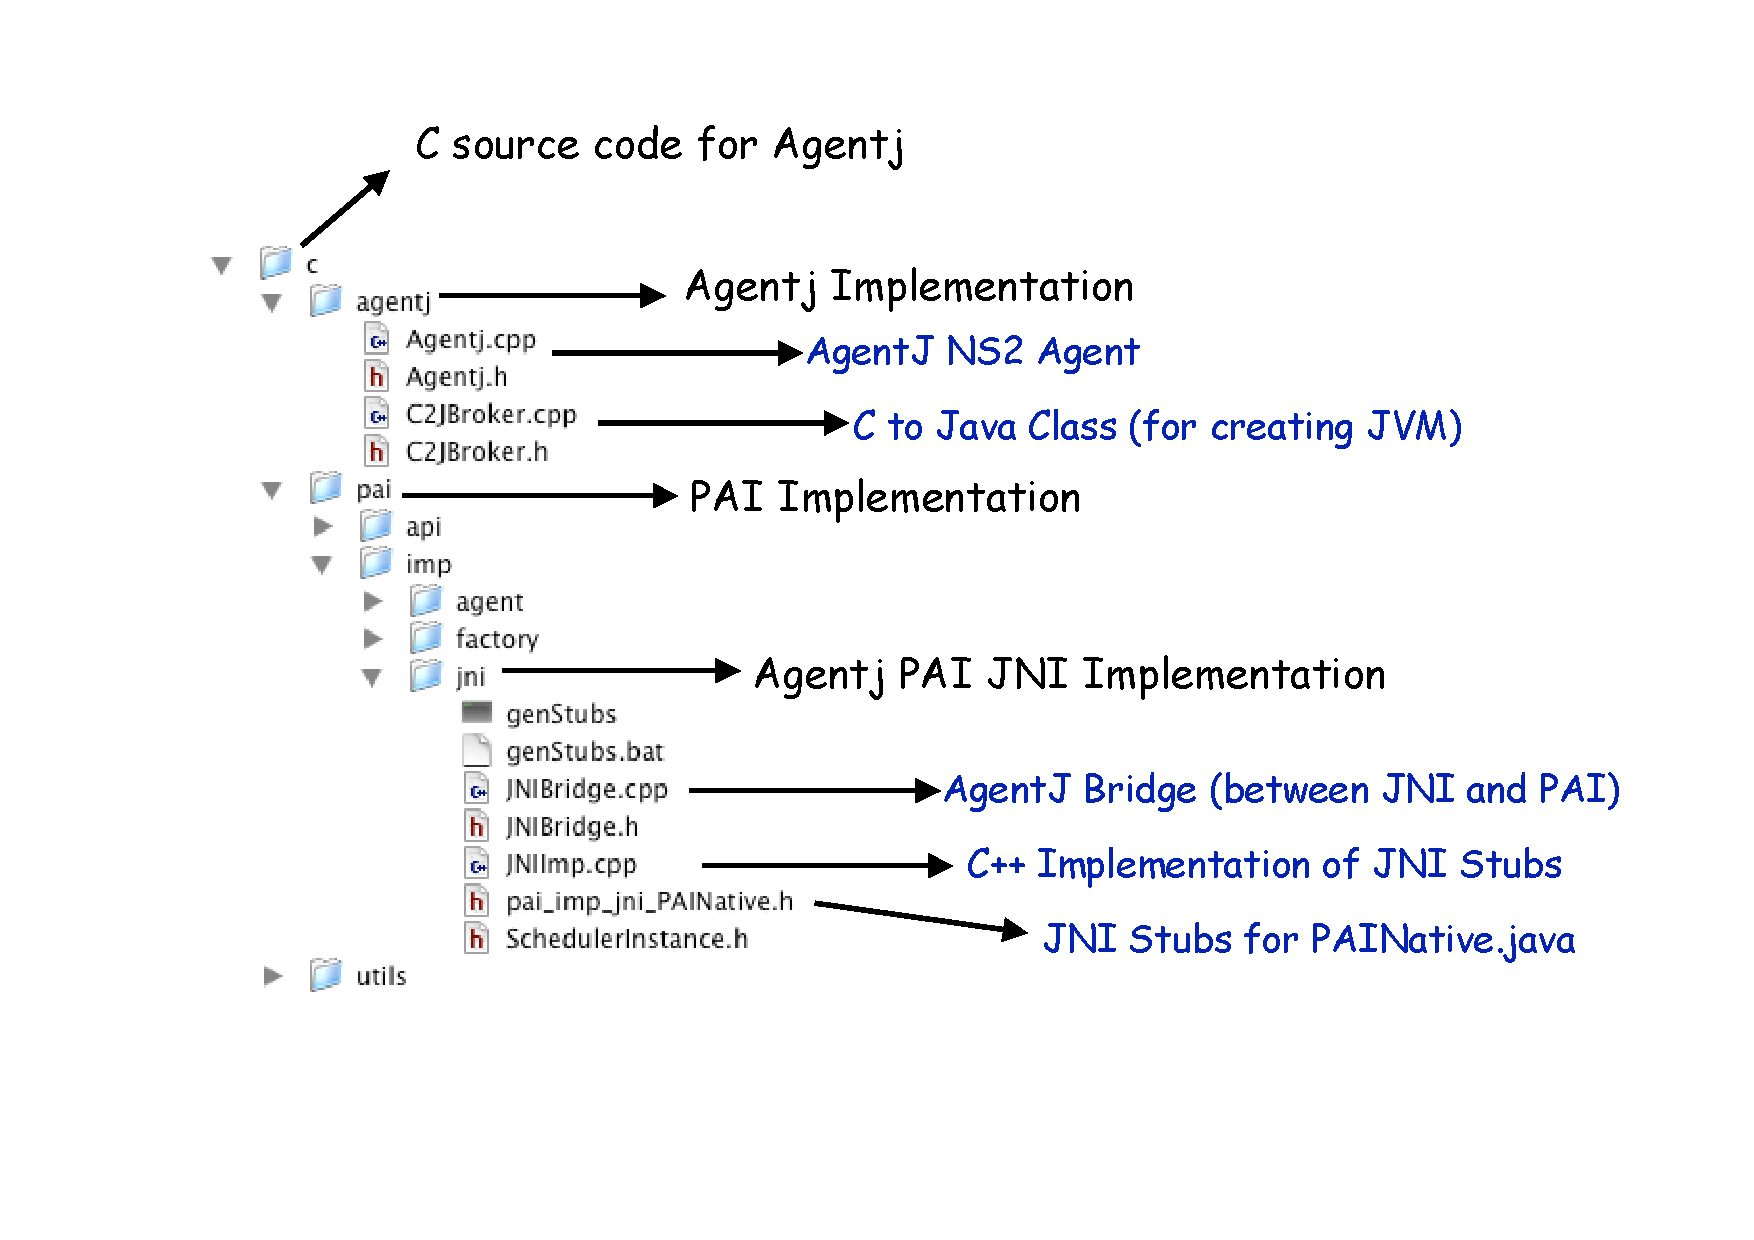
\includegraphics[scale=0.45]{images/agentjCClasses}
\caption{The C++ Classes within \agentj.} 
\label{agentj:fig:CClasses}
\end{figure}

At the top-level, there is a 'java' directory and a 'c' directory. These 
two directory structures are illustrated in Figures \ref{agentj:fig:CClasses} 
for C++ and \ref{agentj:fig:JavaClasses} for Java. At the next level,
both the Java and C source trees are split into two sub-directories,
one containing the classes specific to the implementation of
\agentj and the other to the supporting implementations of
PAI, as illustrated.

\begin{figure}
\centering
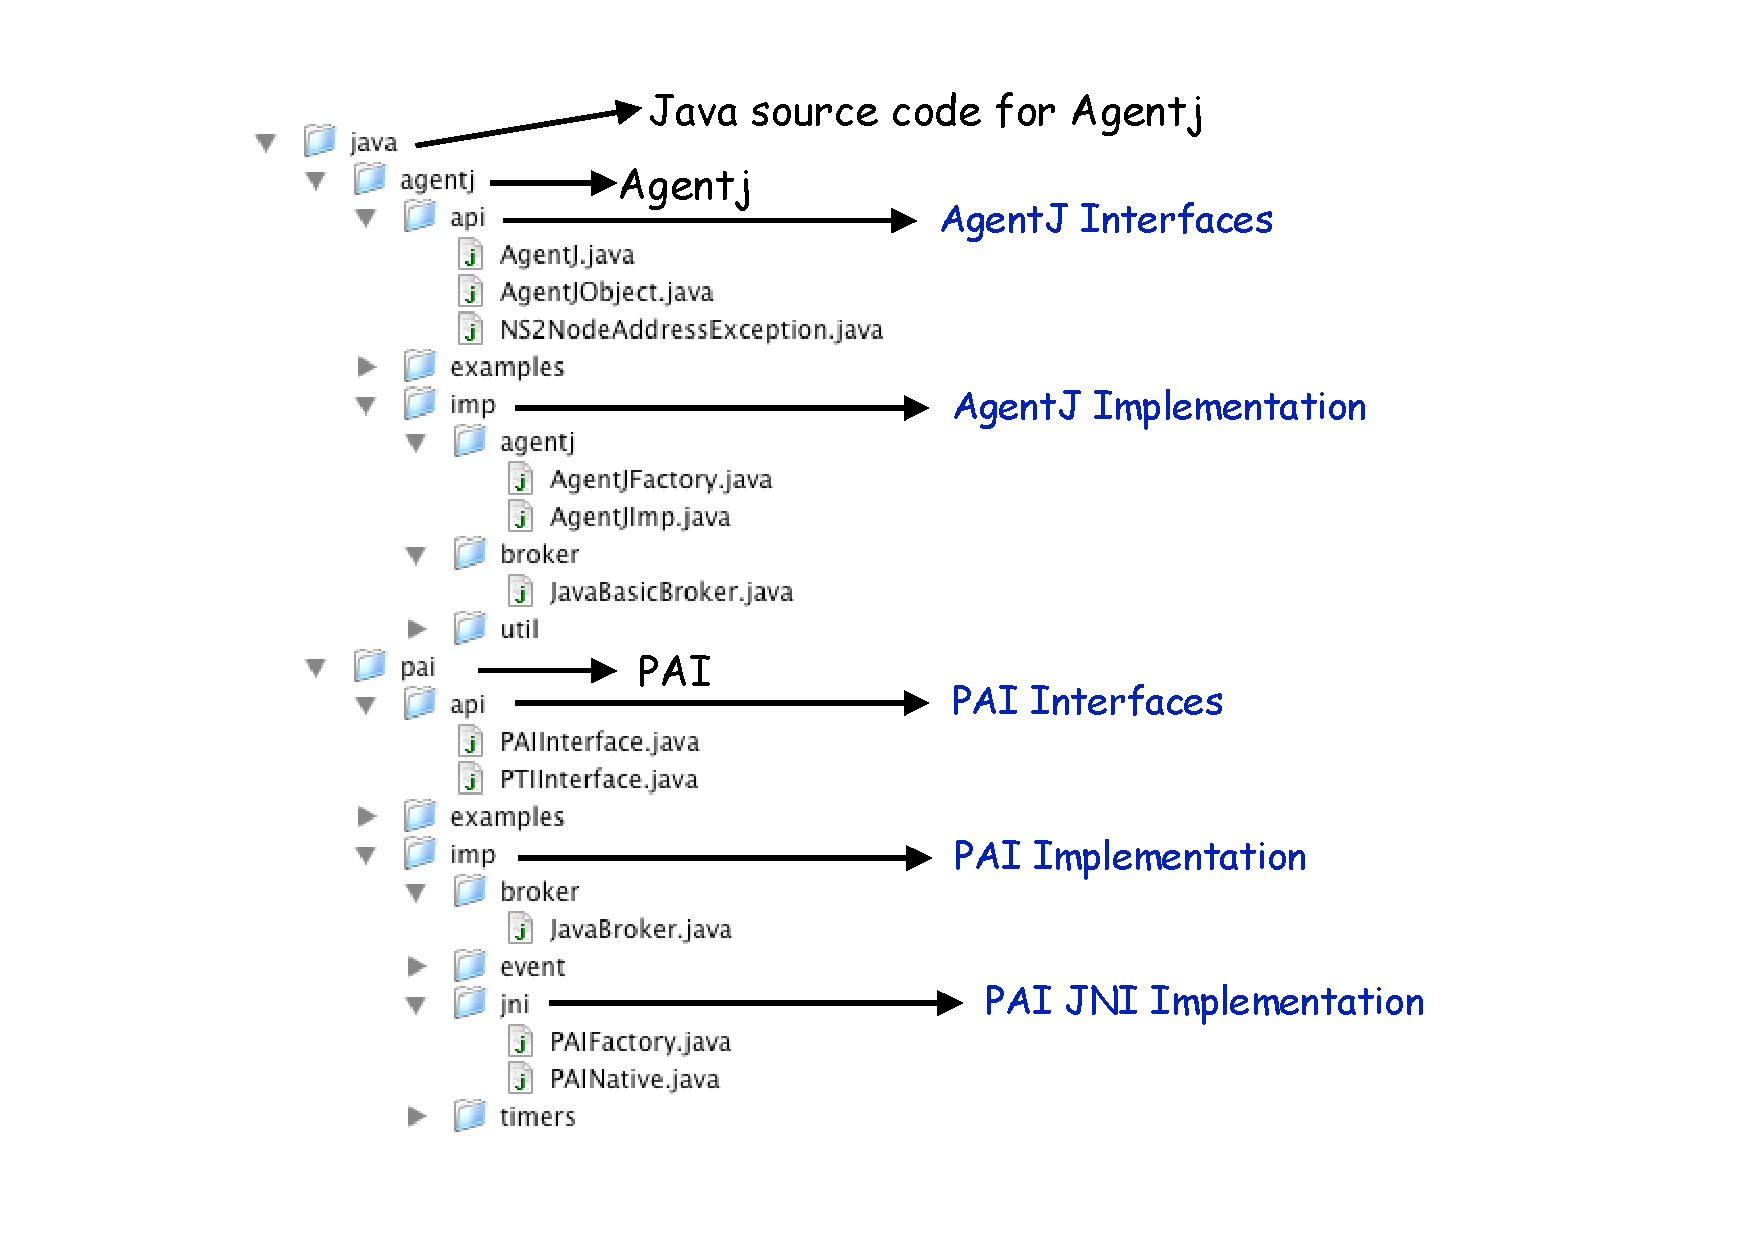
\includegraphics[scale=0.45]{images/agentjJavaClasses}
\caption{The Java Classes within \agentj.} 
\label{agentj:fig:JavaClasses}
\end{figure}


Beyond this, there are subdirectories that correspond to the
particular section of the overall implementation that those
classes are involved with. Therefore, theses directories are
organized as if they were Java packages (and indeed, in Java,
they ARE Java packages). Therefore, APIs (or Java interfaces 
to APIs) are always put in a directory called 'api' and 
implementations of such interfaces are always put in  
directories called 'imp'. Subsequently, implementations of different 
interfaces or APIs are inserted into different sub directories. 

These two Figures will be references in the next section, when we
discuss the specifics about the individual classes which are used
to implement parts of the overall system.
 
\subsection{Key \agentj~Classes}

The central class in \agentj, which implements the bridge between the 
C++ NS2  nodes and Java is \emph{Agentj.cpp} (found in  
\emph{Agentj/src/c/agentj}, see \ref{agentj:fig:CClasses}).  Agentj.cpp
inherits from Protolib's \emph{NsProtoAgent}, which
is a C++ NS2 agent, which can use the Protolib data transport 
implementation e.g. UDP and TCP, within NS2. \emph{Agentj} uses 
the \emph{Agentj} class to attach a Java Object to a C++ agent.  
Thereafter, the Java object itself interfaces through JNI to PAI, 
which in turn uses the Protolib to send the actual data packets. 

\begin{figure}
\centering
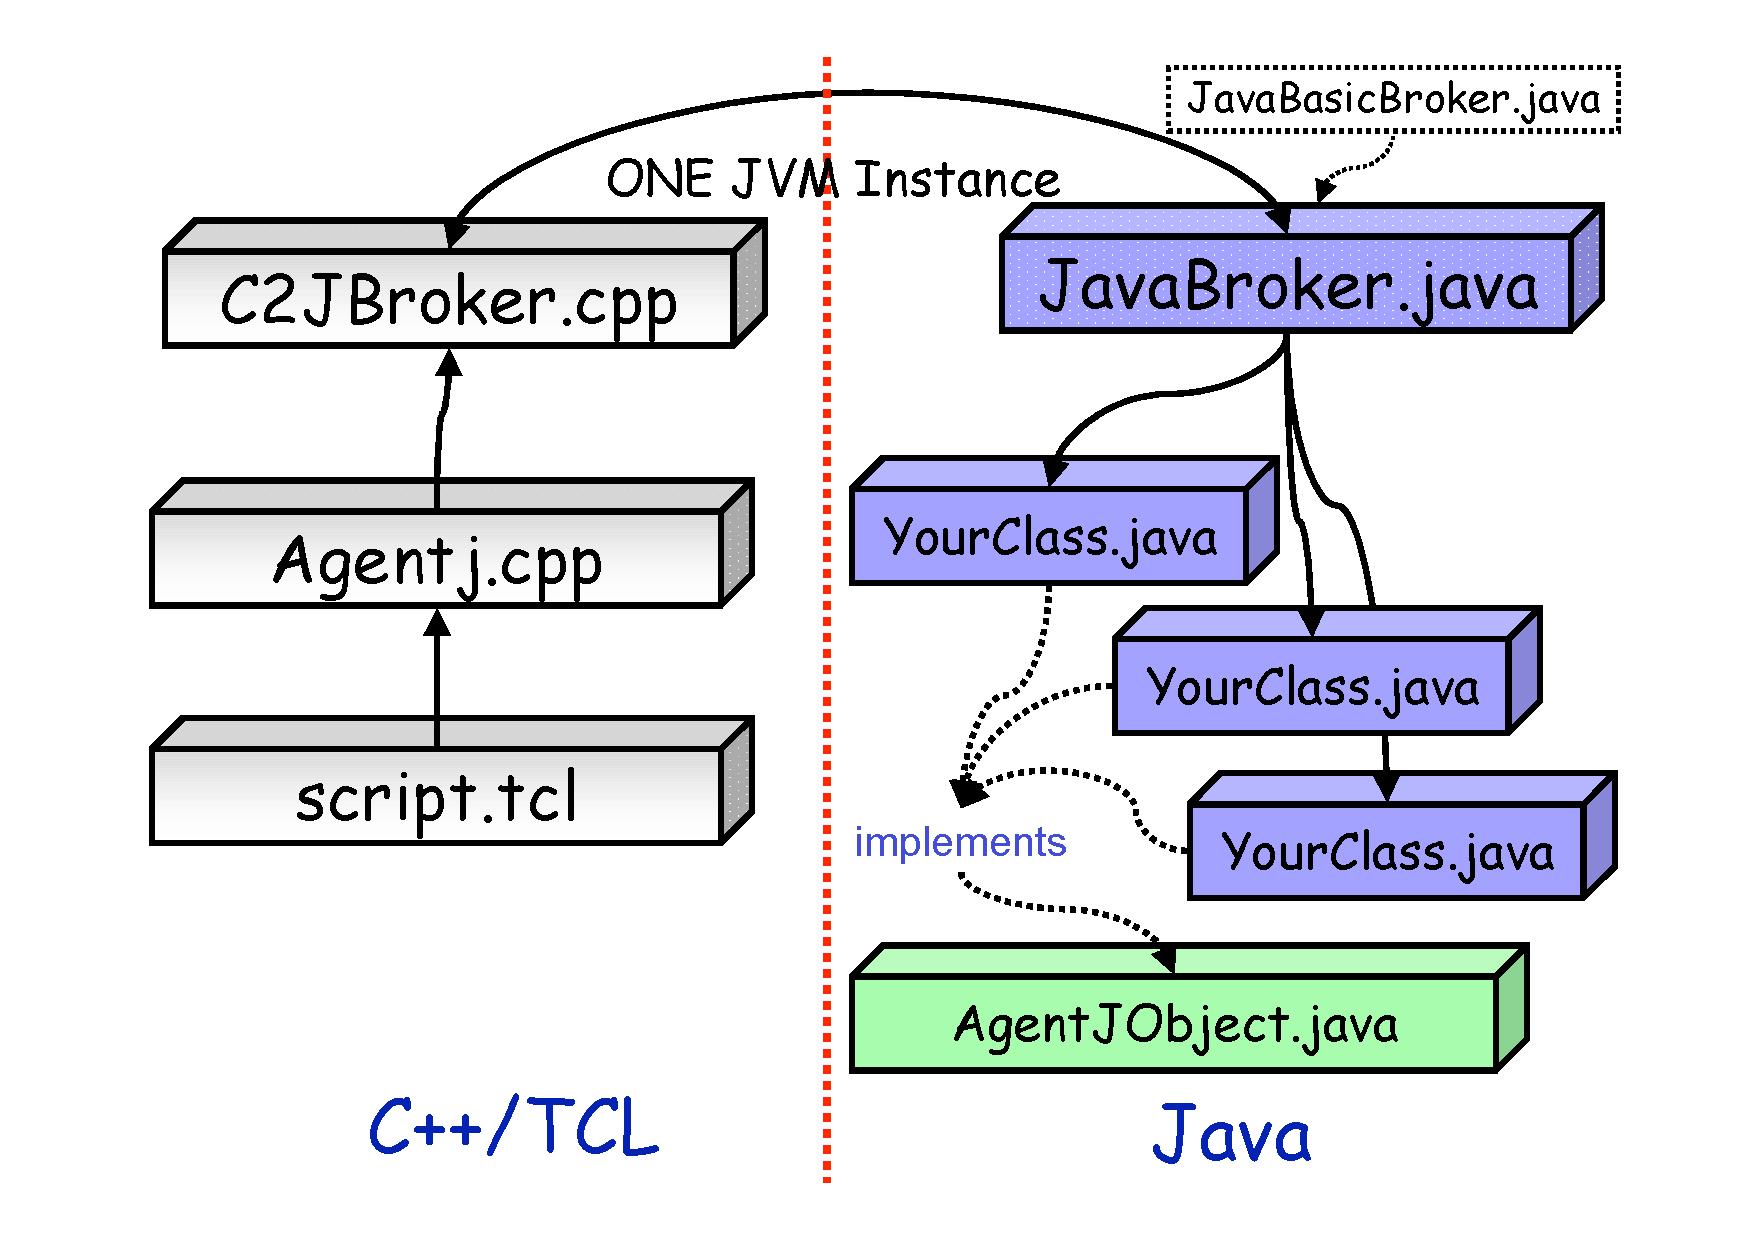
\includegraphics[scale=0.4]{images/agentjClasses}
\caption{The C++ and Java classes used to implement the TCL/C++ and Java
bridging mechanism.} 
\label{agentj:fig:jniClasses}
\end{figure}

As shown in Figure \ref{agentj:fig:jniClasses}, \emph{Agentj} uses the
C2JBroker C++ class to create a Java Virtual Machine (JVM) and 
communicate with the singleton \emph{JavaBroker} Java class.  
C2JBroker simply has these two functions:  it creates a JVM and 
provides a C++ interface for sending messages to the JavaBroker 
Java class. However, it also implements some finer grained 
functionality. C2JBroker initializes \agentj's environment variables.
It parses the LD\_LIBRARY\_PATH and CLASSPATH variables and
passes them to the JVM when it is being created so that the JVM
can use the standard initialization procedures.  It also, sets
up the debugging settings i.e. by checking the AGENTJDEBUG
and AGENTJXMLCONFIG variables (see Chapter \ref{install}).  


The \emph{JavaBroker} Java class allows provides a container 
for the Java objects that \agentj creates during the lifetime of the 
simulation.  A Java Hashtable is used to store each Java object 
along with its identifier, which is the reference to the NS2
agent that this Java object belongs to.  Each NS2 agent can
attach (instantiate) one Java class and therefore there is a 
one-to-one interaction between an NS2 agent and its Java object. 

These interactions are shown in detail in Figure \ref{agentj:fig:jniClasses}. 
Briefly, the programmer attaches the Java class within
the TCL script.  The JavaAgent then passes this data via \emph{C2JBroker}
to the \emph{JavaBroker} Java object. The \emph{JavaBroker} instantiates 
this object on-the-fly from the given class name.  This means that you can
attach multiple Java objects of the same type to every node or you are free
to attach different objects to different NS2 nodes, depending on what you 
want to implement.  For example, you could have a Java data collector 
agent talking to a Java data collection manager node instance. The only 
stipulation on the Java objects being created is that they should implement 
the \emph{AgentJObject} interface.
 
\begin{figure}
\centering
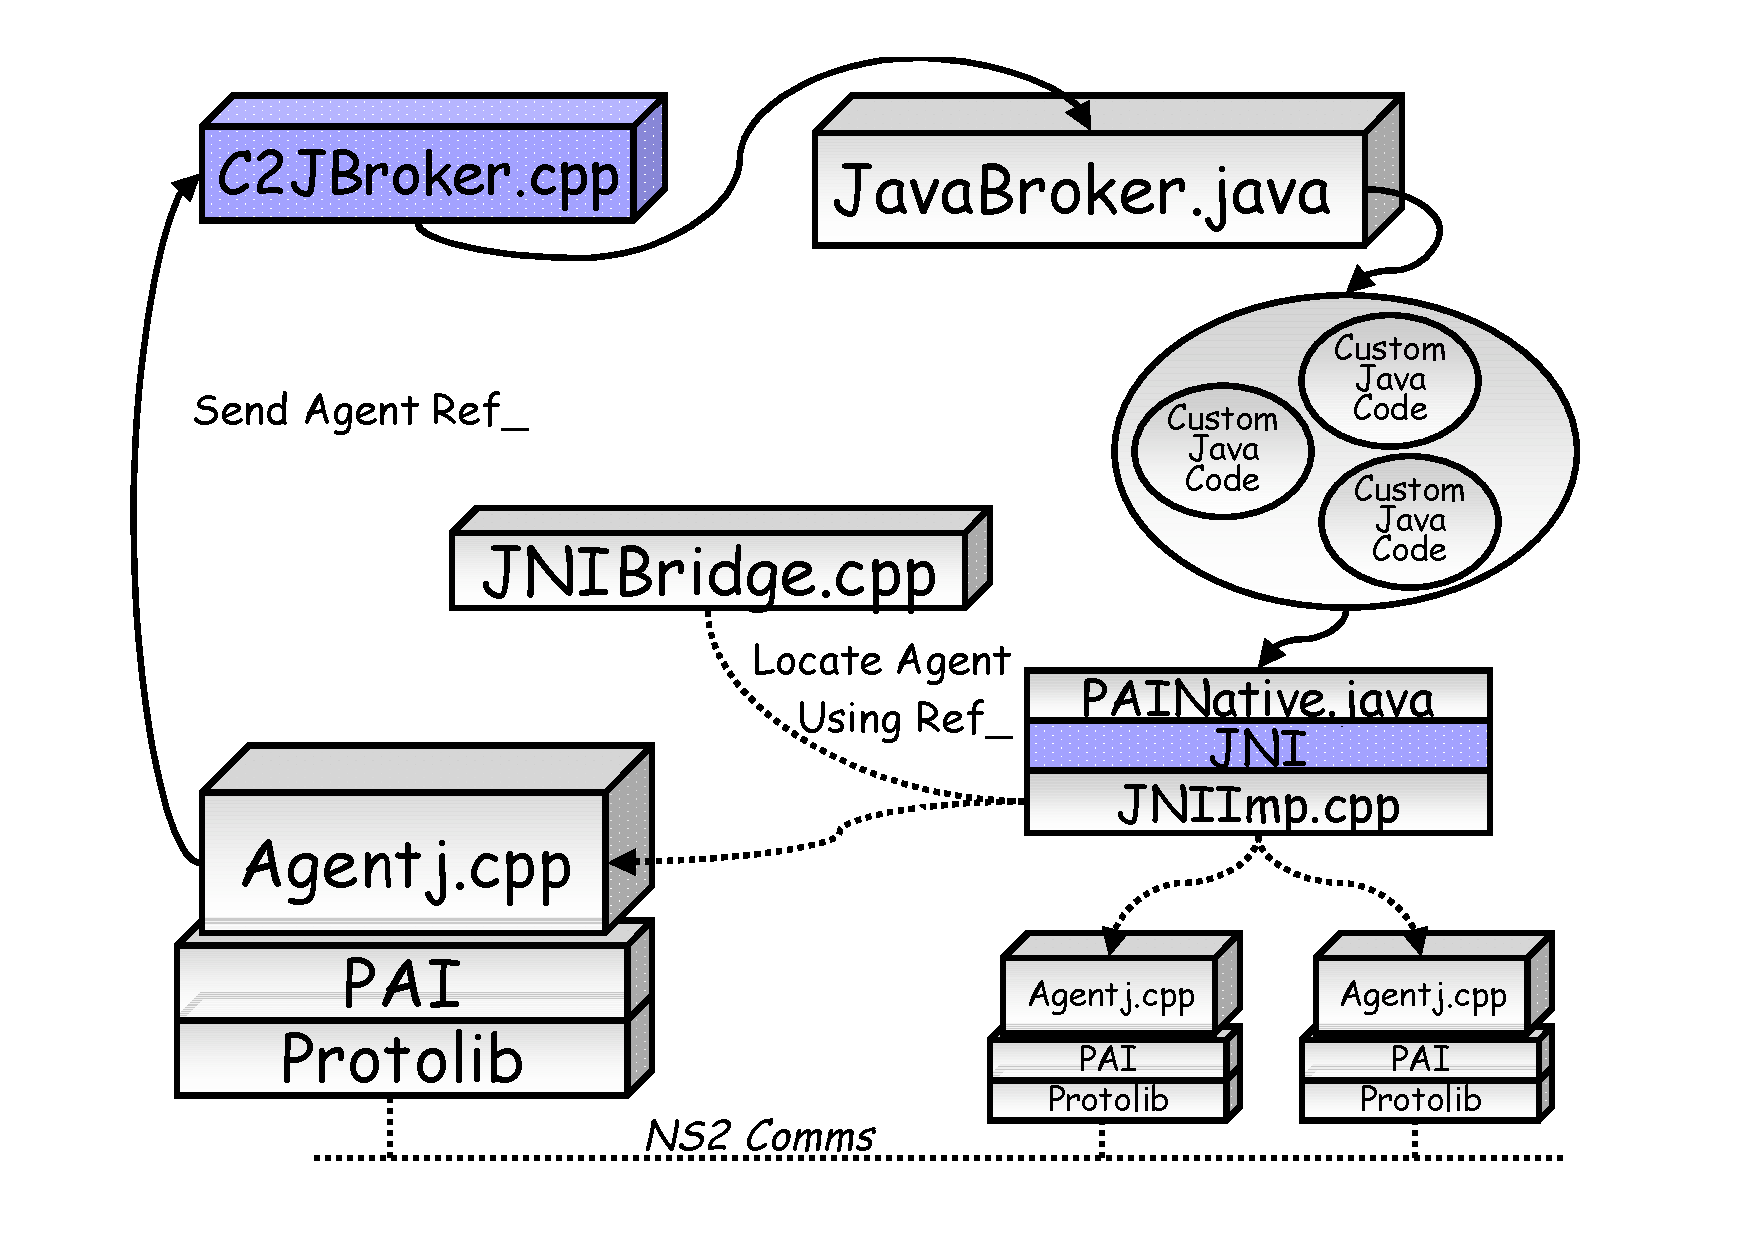
\includegraphics[scale=0.4]{images/agentjOverviewWithClasses}
\caption{The C++ and Java classes shown in the broad overview of \agentj.} 
\label{agentj:fig:agentjOverviewClasses}
\end{figure}


Figure \ref{agentj:fig:agentjOverviewClasses} shows the \agentj architecture
given in Figure \ref{agentj:fig:javaFullOverview} but inserts the various C++ and
Java classes which are used to implement each of the interactions. This clearly illustrates the interaction between
the \emph{Agentj}, \emph{C2JBroker} and \emph{JavaBroker} 
classes. Notice here that also the purpose of the \emph{JavaBroker}
is also illustrated; that is, it acts as a container for the multiple Java
objects (\agentj~nodes) that \agentj~creates. 

Also, depicted here, are the classes involved in the Java and JNI 
implementation of the PAI interface.  The Java PAI interface is outline in 
the next subsection and is implemented by the \emph{PAINative} Java 
class, which binds this interface, through JNI to the underlying C++ 
PAI implementation.  Within this implementation, there are two key 
C++ classes: \emph{JNIImp} and \emph{JNIBridge}. JNIImp is
a direct implementation of the Java native methods contained within
the PAINative Java class, whilst \emph{JNIBridge} provides a 
persistent C++ object for storing information about the state of the
C++ PAI interface during this session.  

For example, \emph{JNIBridge}
contains the list of Java to C++ mappings of the various listeners that
have been attached to the numerous sockets and timers which may
have been created by the Java application.  It also implements the
callbacks to Java, which in turn, result in an event being passed 
to the Java classes which have requested to be notified about 
such events. This is a somewhat complicated procedure because
C++ callbacks to Java have no context, so they must invoke a static
Java method using an identifier notifying it which socket or timer
this event belongs to. From this information, the Java method can
work out which listeners are interested in this event.   


\subsection{The Java PAI interface}
\label{jnipai:jpai}

The Java PAI implementation consists of two Java interfaces:

\begin{itemize}
\item \textbf{PAIInterface:}  interfaces to the communication part of the 
PAI interface (i.e. the sockets).  
\item \textbf{PTIInterface:}  interfaces to the timing part of the 
PAI interface (i.e. the timers).  
\end{itemize}

 
The \emph{PAIInterface} allows the user to create multiple sockets and 
allows multiple socket listeners to be attached to each socket.  This 
functionality is necessary for Java applications and
is illustrated in the P2PS implementation, described in \cite{p2psx}.
The \emph{PTIInterface} does the same for timers.  However,
it is \textbf{important to note} that a user of \agentj does not have
to use these classes directly. In fact, a user should not use these 
classes directly!  They should use the PAI implementations
of the UDP, TCP and timing interfaces for the default Java 
interfaces to these classes e.g. if you want to create a UDP
socket then you should create a \emph{pai.net.DatagramSocket},
which behaves exactly the same as a 
\emph{java.net.DatagramSocket} except that it works within NS2.
The interfaces here merely describe the lower level interfaces and
mechanisms that are used to implement the overall structure.

The Java PAI interface is defined using a collection of Java 
interfaces and uses the \emph{Factory Method Design} pattern 
\cite{designpatterns} in order to create the appropriate underlying
implementation.  This means that other implementations (e.g. a native
Java implementation) could be implemented at a later date.
The application developer however, would not notice this code
change because s/he is working with a consistent interface.  The
JPAI interface can be found in package \emph{pai.api} in the
Java source tree and is listed below:

\footnotesize
\begin{verbatim}

public interface PAIInterface extends PTIInterface {
    void init();
    
    void addPAISocketListener(DatagramSocket sock, PAISocketListener listener);

    void removePAISocketListener(DatagramSocket sock, PAISocketListener listener);

    void open(DatagramSocket sock, int port) throws SocketException;

    DatagramSocket addSocket(int port) throws SocketException;

    void removeSocket(DatagramSocket sock) throws SocketException;

    void setReuseAddress(DatagramSocket sock, boolean on) throws SocketException;

    void setSendBufferSize(DatagramSocket sock, int size) throws SocketException;

    void setReceiveBufferSize(DatagramSocket sock, int size) throws SocketException;

    void setSoTimeout(DatagramSocket sock, int timeout) throws SocketException;

    void send(DatagramSocket sock, DatagramPacket p) throws IOException;

    void receive(DatagramSocket sock, DatagramPacket p) throws IOException;

    void close(DatagramSocket sock);

    void joinGroup(MulticastSocket sock, InetAddress mcastaddr) throws IOException;

    void leaveGroup(MulticastSocket sock, InetAddress mcastaddr) throws IOException;

    void setMulticast(MulticastSocket sock, boolean val);

    public InetAddress getByName(String host) throws UnknownHostException;

    public InetAddress getLocalHost();

    public boolean cleanUp();
    public boolean runBlock();
    public boolean runNonBlock();

    public void setNS2Node(String nodeID);

    public void setNS2Scheduler(String schedulerID);
}
\end{verbatim}
\normalsize
  
Most of the calls are self-explanatory.  PAI uses the Java conventions
for naming the classes e.g. DatagramSocket and MulticastSocket, both found
in the java.net package (see \cite{javaTutorial}). The PAI Java 
implementation reimplements the methods from these classes in order
to use the PAI interface.  This enables the PAI interface to provide the 
functionality but it leaves the Java interface that developers are familiar
with the same. Therefore, to create a Java UDP socket, you simply
instantiate a DatagramSocket, which in turn invokes PAI to create
a C++ PAI socket, which in turn creates a Protolib socket.   

The \emph{PTIInterface} is much simpler:

\footnotesize
\begin{verbatim}

public interface PTIInterface {
    PAITimer addTimer(double delay, int repeat);

    void removeTimer(PAITimer timer);

    void addPAITimerListener(PAITimer timerID, PAITimerListener listener);

    void removePAITimerListener(PAITimer timerID, PAITimerListener listener);

    boolean runTimers();
}

\end{verbatim}
\normalsize

Here, we simply provide a mechanism for creating a simple timer and
allow a Java application to attach multiple listeners to it.
 
This design carries the whole weight of the \agentj implementation.  
To an application, the use of the conventional Java interface for 
creating  UDP sockets means that they require very 
little source code modification in order to use this PAI JNI binding here.
For example, in order to get P2PS working (see \cite{p2psx}) with this 
interface, a new resolver was created for UDP. This was a direct copy 
of the Java UDP resolver code with the occurrences of \emph{java.net} 
replaced with \emph{pa.net}, which enables this new resolver to look in
the appropriateplace for the PAI DatagramSocket class. Everything else 
followed through the various layers and P2PS required no further 
modification at the transport level. This re-implementation of these base 
Java classes can be found in the \emph{pai.net} package in the source tree. 

\section{Conclusion}

In this chapter, an overview of the \agentj~integration was given, from
a conceptual perspective and a source-code perspective. We illustrated
the design and architecture of \agentj~then described in detail the
interaction between the C++ and Java sections of the system.  We then
delved into the Java and C++ classes and outlined the key classes
that implement this functionality and further, outlined the directory structure
for \agentj~ for reference.  We then inserted the names of these classes
back into the architectural overview to give a clear picture of the entire
system and the key components thereof.  Finally, we gave a brief
outline of the Java PAI interface to illustrate the kind of functionality it
provides.
  




\part{Using \agentj}

In this part, we describe \agentj~from a user's perspective.  A typical user of \agentj~would be a programmer of a Java application who would like to simulate their distributed application within NS2.  In this part therefore, we describe how this can be achieved 
and which interfaces need to be implemented in order to build a bridge between NS2 and your distributed Java application.  A comprehensive example of such an integration can be found in the accompanying manual for P2PSX \cite{p2psx}, which integrates a comprehensive P2P middleware system into NS2 using \agentj. 

\chapter{Using \agentj}
\label{jnipai}

Using \agentj, a Java NS2 agent can be attached to an NS2 node and
can be used to integrate any Java application. This chapter gives an 
overview of the interaction between the 
TCL scripts, the C++ NS2 agents and Java objects, which can be accessed from each
NS2 node.  The various code snippets are taken from the \agentj~
source tree and pointers are referenced relative to the
installation directory, when provided. 


\begin{figure}
\centering
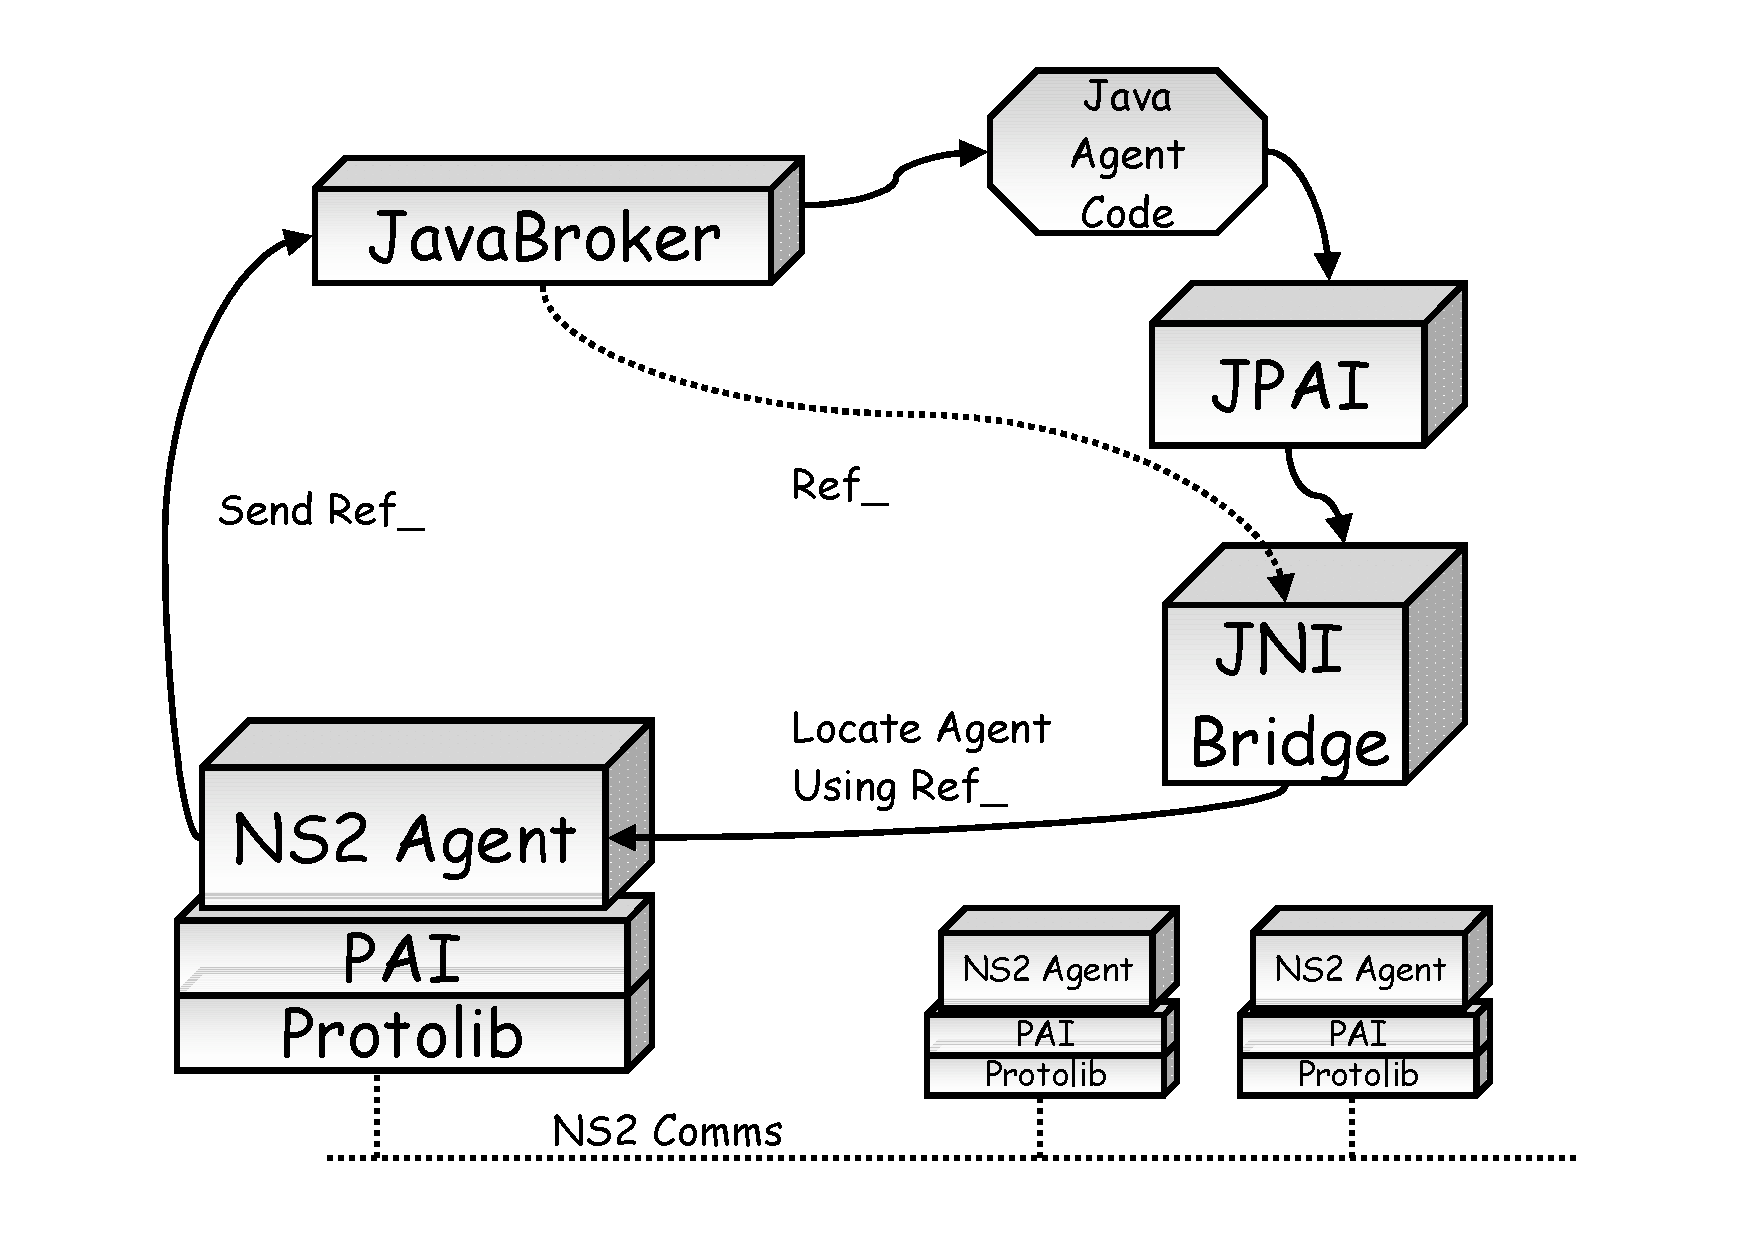
\includegraphics[scale=0.4]{images/agentjJNIOverview}
\caption{An overview PAI is accessed from within a Java node for an NS2 agent} 
\label{jnipai:fig:overview}
\end{figure}

Figure \ref{jnipai:fig:overview} shows an overview of the 
interaction between the C++ agents, the \emph{JavaBroker}
and the Java PAI bridge that enables this to be interfaced with
the C++ PAI library. As discussed briefly in the previous
chapter, the C++  \emph{JavaAgent} passes the pointer to the C++
agent to the  \emph{JavaBroker} when it requests to create and
attach a Java agent to the NS2 node.  

The  \emph{JavaBroker}
class uses this pointer to store the created Java object in
a hashtable for lookup but also pass this references across to
the JNI interface, when a Java object requires the use of 
the PAI interface. This enables the JNI interface to locate the
node that created the Java object and therefore whom is
indirectly issuing the commands, which ensures that 
the data being sent through the sockets is sent from 
the correct node.  The PAI interface sends these commands
to the Protolib library, which in turn, uses the Protolib NS2 UDP
implementation to send the data between the NS2 nodes.


\section{Invoking Java Agents from NS2 Agents}
\label{jni:invoke}

Figure \ref{jni:fig:javaVM} shows interaction between an agent and 
its associated Java class.  The programmer who wishes to use this
Java functionality within their NS2 simulations only needs to be 
concerned within their NS2 TCL script and their Java class that 
implements the behaviour. The relationship between an Ns2 agent 
and its Java class is very similar to the relationship between an NS2
TCL script and its associated C++ class (i.e. an NS2 agent) which 
implements the same kind of interaction through sending text
commands between the two. The Java interface
employs the same mechanism to bridge these different 
programming languages. The C++ agent (JavaAgent) simply acts
as a go-between and passes that commands across to the
appropriate Java object. 

\begin{figure}
\centering
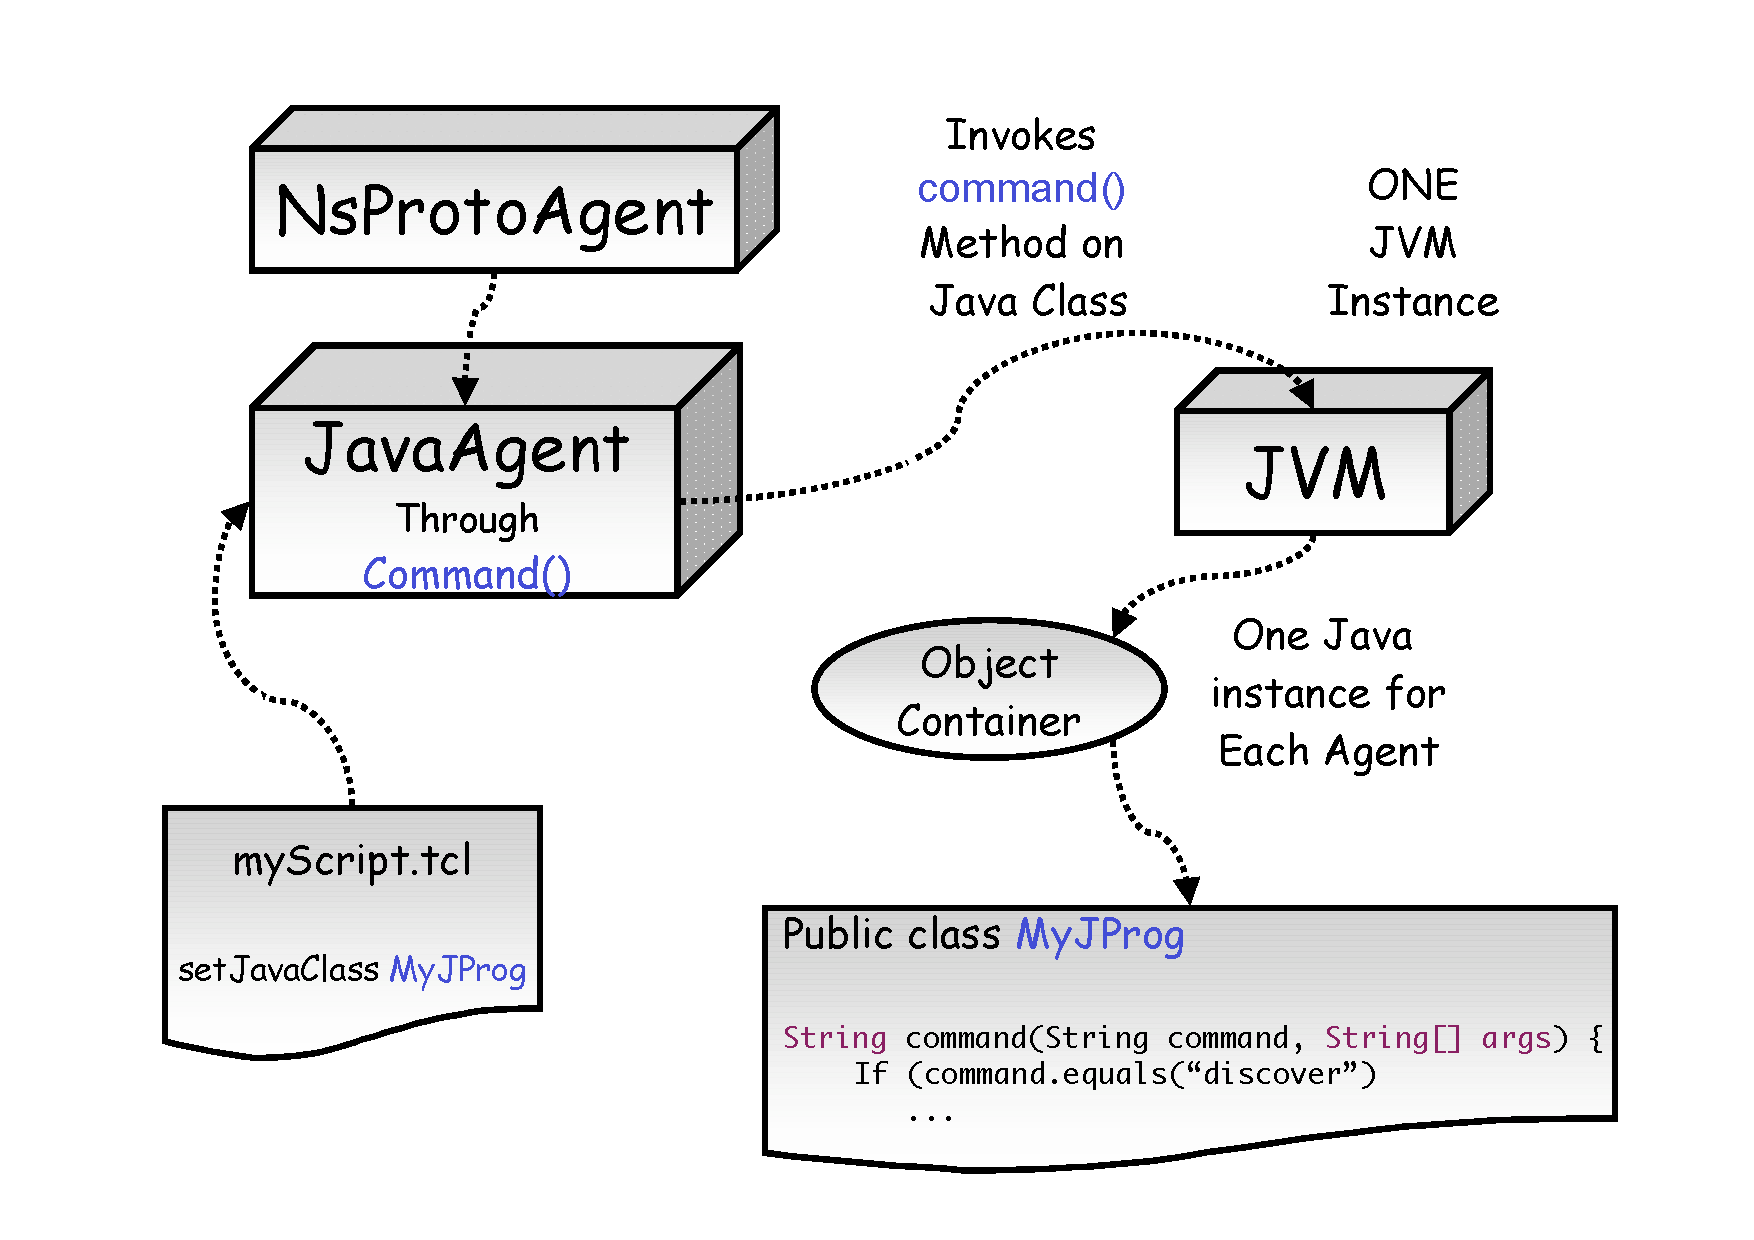
\includegraphics[scale=0.4]{images/agentuserJVM}
\caption{The interface to a Java program for an agent employs 
a similar interface to that of NS2 when communicating between 
the TCL scripts and the C++ classes. } 
\label{jni:fig:javaVM}
\end{figure}

Therefore, the interface between the NS2 \emph{JavaAgent} 
and the chosen Java Class it will interact with, uses the same 
command-style interface as the TCL-C++ interface for invoking 
functionality on NS2 agents. This command-style interaction 
satisfies some essential constraints:

\begin{itemize}
\item \textbf{Flexibility:} it will keep the flexibility of being able to use NS2 agents in any way programmer sees fit - the Java extensions are optional and any agent extending
the \emph{JavaAgent} can choose to use this functionality. However, the core
C++ agent code can be programmed to incorporate and other functionality 
needed beyond the scope of Java. 
\item  \textbf{Simplicity:} the scalability issues and framework for interacting with
the Java objects can easily be hidden behind the container C++ and Java classes 
- the programmer does not need to be aware of their presence.
\item  \textbf{Familiarity:} this mechanism allows communication between the 
NS2 agent and any attached Java class through the same familiar interface as NS2 programmers interface between the TCL scripts and C++ agents now.
\end{itemize}

\begin{figure}
\centering
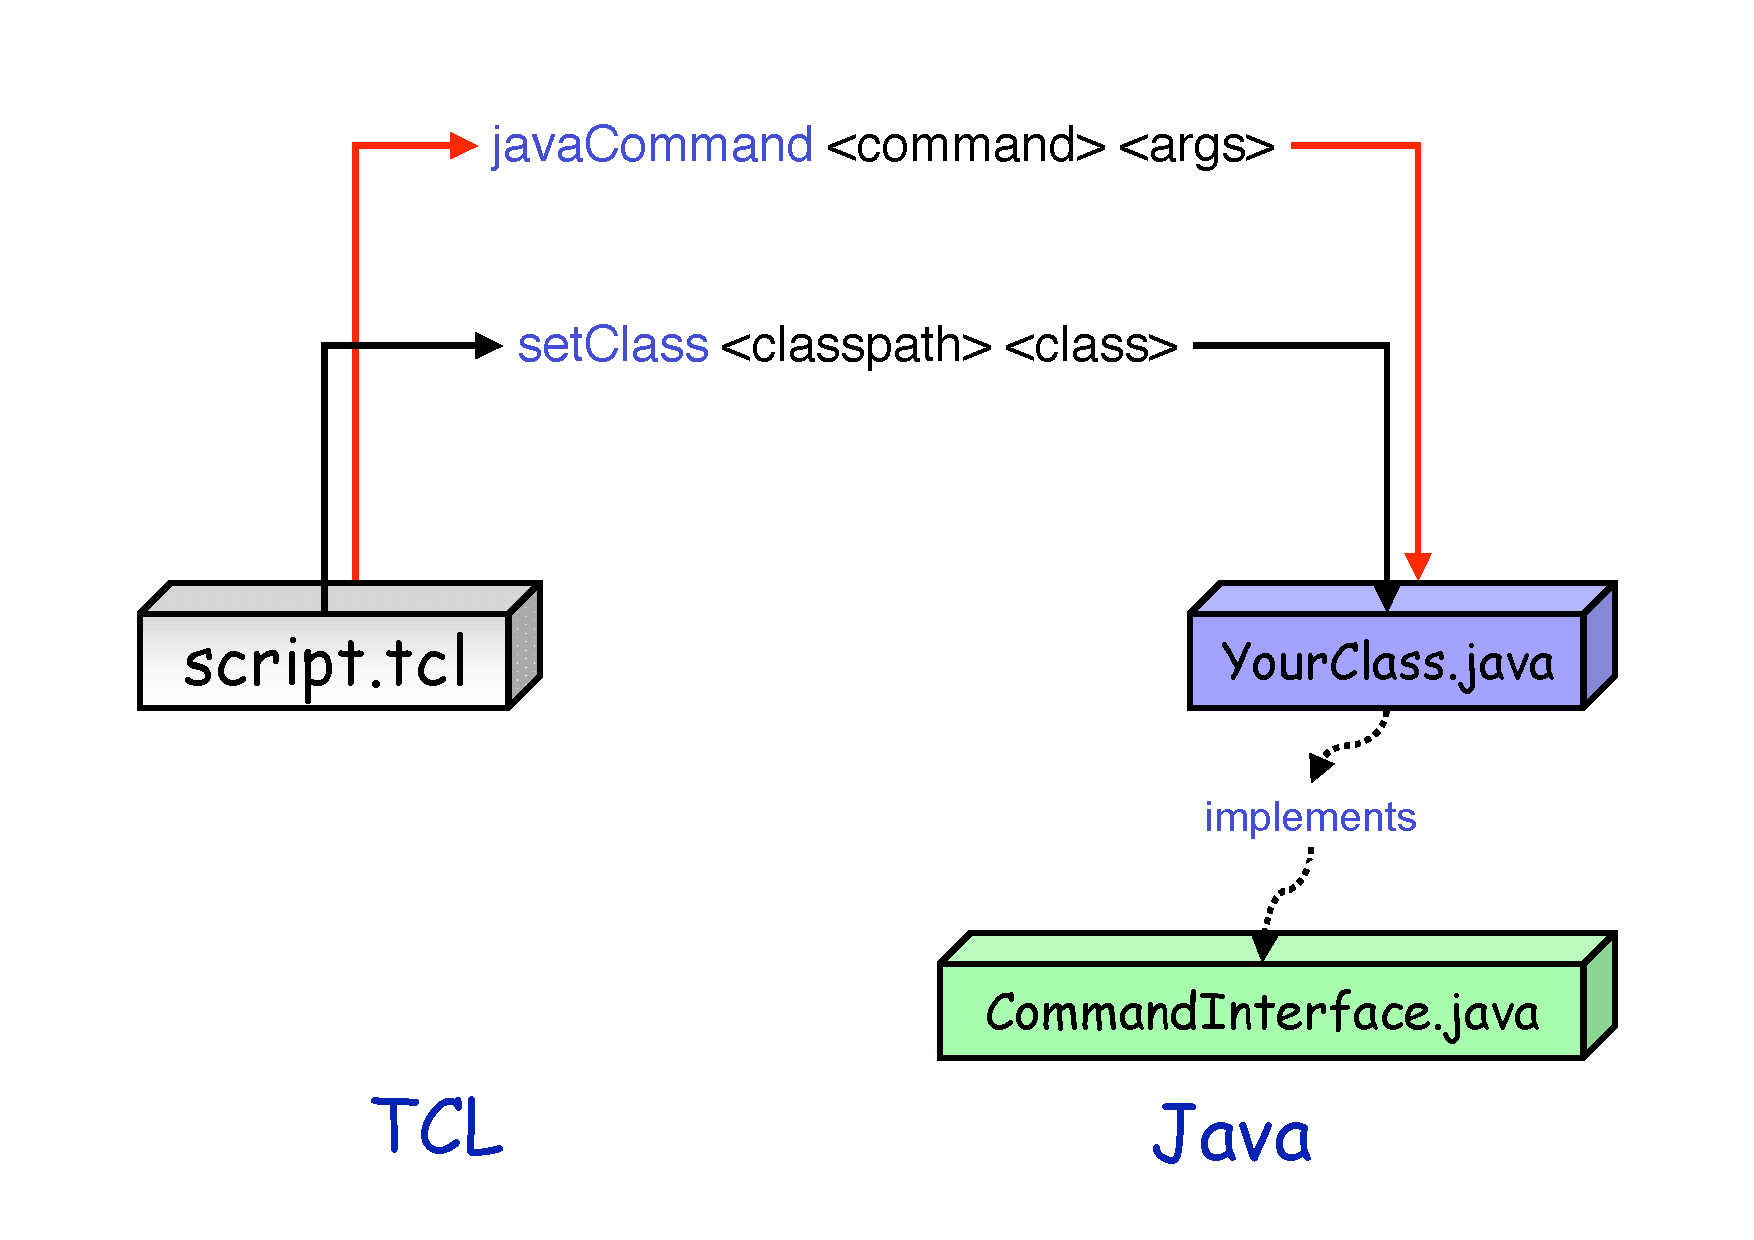
\includegraphics[scale=0.4]{images/agentuserOverview}
\caption{The user's view of the interaction between the NS2 agent/script and
the Java class associated with that NS2 node.} 
\label{jni:fig:javaTCLJava}
\end{figure}

This interaction is shown in Figure \ref{jni:fig:javaTCLJava}, which shows 
some  \emph{JavaAgent} commans for specifying and attaching a Java
object and for sending it commands.  These are the minimum commands 
needed in order to use your Java object.  Each Ns2 node creates a 
Java object of its own choice by using the TCL command:

\footnotesize
\begin{verbatim}
setClass <classpath> <class>
\end{verbatim}
\normalsize

\noindent which allows the Java classpath to be set along with the name of the Java class to be instantiated for this NS2 node. Once the Java object has been created,
commands can be sent by using the TCL command:

\footnotesize
\begin{verbatim}
javaCommand <command> <args>
\end{verbatim}
\normalsize

\noindent which would invoke the java command with the associated 
arguments. There are also other commands implemented that allow you to
specify the delimiter to make it easier to chunk your arguments in a
flexible way and for creating a trigger mechanism.  The following 2
sections illustrate these commands through the use of example
TCL and Java codes and the next chapter illustrates how you
can extend the Java functionality to use PAI in order to send
data between your Java objects through the NS2 subsystem.


\section{Creating and Attaching a Java Agent }
\label{jni:basic}

This is a \emph{Hello World} example that demonstrates how
to specify the Java classpath and choose a Java class to instantiate
and attach to your C++ agent. It then implements a simple \emph{hello}
function which is invoke on the Java object. 

\subsection{The TCL Side}
\label{jni:tclside}

The following is the TCL script part of the implementation, which creates two 
\emph{JavaAgent} NS2 nodes that each create a \emph{SimpleCommand} 
Java object and then invoke a 'hello' command on that object. This
example can be found in examples/pai/javaAgent/startJava.tcl.)

\footnotesize
\begin{verbatim}

puts "Starting..."   

# Create a simulator instance
set ns_ [new Simulator ]

# Create two nodes
set n1 [$ns_ node]
set n2 [$ns_ node]

# Put a link between them
$ns_ duplex-link $n1 $n2 64kb 100ms DropTail
$ns_ queue-limit $n1 $n2 100
$ns_ duplex-link-op $n1 $n2 queuePos 0.5
$ns_ duplex-link-op $n1 $n2 orient right

puts "Creating JavaAgent NS2 agents and attach them to the nodes..."   
set p1 [new Agent/JavaAgent]
$ns_ attach-agent $n1 $p1

set p2 [new Agent/JavaAgent]
$ns_ attach-agent $n2 $p2

puts "CREATED OK          ....... ..." 
    
# Initialize each broker telling it what its NS2 address is

puts "In script: Initializing  ..." 
	
$ns_ at 0.0 "$p1 initAgent"
$ns_ at 0.0 "$p2 initAgent"

puts "Setting Java Object to use by each agent ..." 

$ns_ at 0.0 "$p1 setClass 
/Users/scmijt/Apps/nrl/p2ps-ns2/classes pai.examples.ns2.SimpleCommand"

$ns_ at 0.0 "$p2 setClass 
/Users/scmijt/Apps/nrl/p2ps-ns2/classes pai.examples.ns2.SimpleCommand"

# send a message to each agent and tell it to print it to the screen
# This is a "HelloWorld" program for JavaAgents

$ns_ at 0.0 "$p1 javaCommand hello AStringFromP1" 
$ns_ at 0.0 "$p2 javaCommand hello AStringFromP2" 

$ns_ at 10.0 "finish $ns_"

proc finish {ns_} {
$ns_ halt
delete $ns_
}

$ns_ run
\end{verbatim}
\normalsize

The Java agent parts can be seen in this example.  The \emph{setClass}
function sets the classpath to the \emph{p2ps-ns2} installations classes 
directory.  Here, the actual java class that this node will be using is 
specified as \emph{pai.examples.ns2.SimpleCommand}.  Note 
here that you can load  in classes that are contained in any 
java package that you wish as long as you follow the Java 
conventions for locating the compiled versions of these classes.

Once the Java classes have been located, you can then execute various 
commands by using the \emph{javaCommand} instruction.  Here we
ask the Java class to execute a \emph{hello} command and pass
a string as an argument, identifying the node that is sending the message 
i.e. \emph{AStringFromP1}.  This simple example demonstrates that
two Java objects have been created, one for each node and each Java
object has been correctly associated or bound to the particular NS2
node.

\subsection{The Java Side}
\label{jni:javaside}

On the java side of things each object you want to talk to must implement a 
standard interface called "CommandInterface" which enforces that every Java
object implementing this interface implements this command method:

\footnotesize
\begin{verbatim}
package pai.broker;

public interface CommandInterface {

    public String command(String command, String value);
}
\end{verbatim}
\normalsize

Every class that you wish to be used from an NS2 agent must implement
this Java interface so that it can understand the instructions that are sent
to it. Below, an example Java class is given to illustrate the code involved 
in this process (the actual Java code for this and all other examples 
\sloppypar can be found in the \emph{src/jpai/pai/examples/ns2} directory):

\footnotesize
\begin{verbatim}

package pai.examples.ns2;

import pai.broker.CommandInterface;

public class SimpleCommand implements CommandInterface {

    static int count=0;

    int myID;

    public SimpleCommand() {
        ++count;
        myID=count;
    }

    public String command(String command, String args[]) {

        if (command.equals("hello"))
            System.out.println("SimpleCommand(" + myID + ") 
            					called with Val: " + args[0]);

        return "All called ok from node " + myID;
    }
}

\end{verbatim}
\normalsize

As you can see, this is extremely simple, the C++ and Java JVM class take care of all
the complexity. In the command method, you can implement any behaviour you
want. You can also return a \emph{String} to your C++ 
program as indicited. This could allow you, for example, to discover other 
NS2 nodes using P2PS and then return their
address to your C++ agent and keep the control at this point (helpful for 
non-java programmers!).


\section{Changing the Command Delimiter }
\label{jni:delimiter}

This example demonstrates how you would change the delimiter used
to separate command arguments sent to your Java application.   
The default is to use a white space (as in NS2) to automatically 
parse the arguments and send them as a sequence of arguments
to your agent or Java object.  Within the Java NS2 implementation
however, this choice is left up to the programmer.  Therefore,
you could specify for example a '-' symbol as a delimeter and
a sequence such as this

\begin{verbatim}
8 - cherry apple oranges - to eat
\end{verbatim}

\noindent would be parsed and sent to you program as 3 strings:

\begin{verbatim}
8
cherry apple oranges
to eat
\end{verbatim}

This allows more flexibility in the way you send instructions to your Java
code because it does not limit the input to contiguous strings. The example
given below demonstrates how this is achieved from the TCL and Java 
sides.

\subsection{The TCL Side}
\label{jni:tclside}

The following is the TCL script part of the implementation, which creates two 
\emph{JavaAgent} NS2 nodes that each create a \emph{ChangeDelimiter} 
Java object and then change the delimiter of one of the nodes in order
to split up the input with respect to a '-' symbol.   Note that setting
delimiters is a global process and therefore can be set through 
any node and will be applied to all nodes. This
example can be found in examples/pai/javaAgent/changeDelimiter.tcl)

\footnotesize
\begin{verbatim}
puts "Starting..."   

# Create simulator instance
set ns_ [new Simulator]

# Create two nodes
set n1 [$ns_ node]
set n2 [$ns_ node]

# Put a link between them
$ns_ duplex-link $n1 $n2 64kb 100ms DropTail
$ns_ queue-limit $n1 $n2 100
$ns_ duplex-link-op $n1 $n2 queuePos 0.5
$ns_ duplex-link-op $n1 $n2 orient right
   
puts "Creating JavaAgent NS2 agents and attach them to the nodes..."   
set p1 [new Agent/JavaAgent]
$ns_ attach-agent $n1 $p1

set p2 [new Agent/JavaAgent]
$ns_ attach-agent $n2 $p2
    
puts "In script: Initializing  ..." 
	
$ns_ at 0.0 "$p1 initAgent"
$ns_ at 0.0 "$p2 initAgent"

puts "Setting Java Object to use by each agent ..." 

$ns_ at 0.0 "$p1 setClass 
/Users/scmijt/Apps/nrl/p2ps-ns2/classes pai.examples.ns2.ChangeDelimiter"

$ns_ at 0.0 "$p2 setClass 
/Users/scmijt/Apps/nrl/p2ps-ns2/classes pai.examples.ns2.ChangeDelimiter"

# Delimiters are global and can be set through any node

$ns_ at 0.0 "$p1 javaCommand setDelimiter -" 

$ns_ at 0.0 "$p2 javaCommand hello A-String-From-P2" 

$ns_ at 10.0 "finish $ns_"

proc finish {ns_} {
$ns_ halt
delete $ns_
}

$ns_ run
\end{verbatim}
\normalsize

The Java classes are located and instantiate as previous. Now, we can
use the \emph{javaCommand setDelimiter} instruction to change
the delimiter.  We set this to '-' and then send a single contiguous string
to node p2 (A-String-From-P2) by using the 'hello' command.  Now
instead of passing this as a single string (as you would get in the NS2 
C++ binding), you would get 4 separate string send to your program,
which can be accessed individually, for example, as:

\begin{verbatim}
A
String
From
P2
\end{verbatim}

\subsection{The Java Side}
\label{jni:javaside}

On the java side \emph{ChangeDelimiter.java} implements the
"CommandInterface" to identify that it can process commands:

\footnotesize
\begin{verbatim}
package pai.examples.ns2;

import pai.broker.CommandInterface;

public class ChangeDelimiter implements CommandInterface {

    static int count=0;

    int myID;

    public ChangeDelimiter() {
        ++count;
        myID=count;
    }

    public String command(String command, String args[]) {

        if (command.equals("hello")) {
            System.out.println("Command has "
                    + args.length + " arguments");
            for (int i=0; i<args.length; ++i) {
                System.out.println("Arg[" + i + "] = " + args[i]);
            }
        }

        return "All called ok from node " + myID;
    }
}

\end{verbatim}
\normalsize

Here, the 'hello' command simply processes through the arguments and
prints each to the screen on a separate line. Therefore, running the script 
will produce the following output:

\footnotesize
\begin{verbatim}

In script: Initializing  ...
Setting Java Object to use by each agent ...
Classpath is -Djava.class.path=/Users/scmijt/Apps/nrl/p2ps-ns2/classes
command has 4 arguments
Arg[0] = A
Arg[1] = String
Arg[2] = From
Arg[3] = P2

\end{verbatim}
\normalsize

\section{Conclusion}

Then, two different examples were provided that illustrate how one would
attach a Java object to an NS2 node and how one can execute Java
commands on that object.  Lastly, an example was given that demonstrates
how you can change the delimiter used to parse the list of arguments you
can send to your Java object.  This employs a flexible mechanism that 
can use any string as a delimiter to send lists or sentences to your
Java object without having to parse further. 



\chapter{Advanced \agentj}
\label{jnipai}

\section{\agentj and PAI}

In the last section, we discussed the way Java objects could be
attached to Java agents and invoke from within NS2 simulations.
In this chapter, an overview of how such Java nodes can be used 
to send packages between NS2 nodes by using the PAI interface,
described in Chapt. \ref{pai}.  The Java interface contains a
an interface to PAI through JNI that enables the Java objects
to create sockets, attach listeners to the sockets and trigger 
events.

\subsection{Using the Java PAI Interface in Ns2 Java Objects}
\label{jnipai:jpaireqs}
 
Each Java objects that has been attached to an NS2 node
must implement the \emph{PAIAccessInterface} given
below, which can be found in the pai.broker package within the
source tree:

\footnotesize
\begin{verbatim}
package pai.broker;

import pai.api.PAIInterface;

public interface PAIAccessInterface {

    public void setPAI(PAIInterface pai);
}

\end{verbatim}
\normalsize


\emph{PAIAccessInterface} provides a mechanism for the 
\emph{JavaBroker} object to create a \emph{PAIInterface} 
object to the JNI PAI implementation and pass this reference 
to your Java code.  You can then use this reference 
directly to make PAI calls just as you would if you were 
using PAI directly.

This mechanism managers the creation and deletion of the
PAI JNI implementation and sets variables in the JNI before
each invocation so that it has the correct reference to the 
object it is dealing with at that moment.  Briefly, the 
\emph{JavaBeker} only create \textbf{one} instance of
the PAI JNI implementation. This means that before each
call it must set the reference to the actual NS2 node it is
about to issue a command to enabling the interface to 
create the appropriate binding to PAI at the lower levels.
This design adds a small overhead to each call but saves
a substantial amount of memory since it efficiently uses
one instance of the code rather that one for each node,
which would increase memory consumption greatly (i.e.
image if you had thousands of nodes).


\section{Example 1: Sending Data From One Node to Another}
\label{jni:node2node}

This example uses the Java \emph{PAICommands} class to 
send data between two NS2 nodes.  The actual Java
code specifies which nodes to communicate with.
This simple example demonstrates how Java objects
can be attached to an NS2 nodes and used to 
create sockets and send data between nodes.

\subsection{The TCL Side}
\label{jni:tclside}

The following is the TCL script part of the implementation, which creates two 
\emph{JavaAgent} NS2 nodes attaches the PAICommands Java object
to them, initializes them and then sends data from the first node to
the second by setting the NS 2 address of the second node directly from
the script, using the \emph{setSendTo} command.

\footnotesize
\begin{verbatim}
# Create multicast enabled simulator instance
set ns_ [new Simulator]

# Create two nodes
set n1 [$ns_ node]
set n2 [$ns_ node]

# Put a link between them
$ns_ duplex-link $n1 $n2 64kb 100ms DropTail
$ns_ queue-limit $n1 $n2 100
$ns_ duplex-link-op $n1 $n2 queuePos 0.5
$ns_ duplex-link-op $n1 $n2 orient right

puts "Creating JavaAgent NS2 agents and attach them to the nodes..."   
set p1 [new Agent/JavaAgent]
$ns_ attach-agent $n1 $p1

set p2 [new Agent/JavaAgent]
$ns_ attach-agent $n2 $p2

puts "In script: Initializing agents  ..." 
	
$ns_ at 0.0 "$p1 initAgent"
$ns_ at 0.0 "$p2 initAgent"

puts "Setting Java Object to use by each agent ..." 

$ns_ at 0.0 "$p1 setClass 
/Users/scmijt/Apps/nrl/p2ps-ns2/classes pai.examples.ns2.PAICommands"
$ns_ at 0.0 "$p2 setClass 
/Users/scmijt/Apps/nrl/p2ps-ns2/classes pai.examples.ns2.PAICommands"

puts "Starting simulation ..." 

$ns_ at 0.0 "$p1 javaCommand init"
$ns_ at 0.0 "$p2 javaCommand init"

$ns_ at 0.0 "$p1 javaCommand setSendTo [$n2 node-addr]"
$ns_ at 0.0 "$p1 javaCommand start"

$ns_ at 10.0 "finish $ns_"

proc finish {ns_} {
$ns_ halt
delete $ns_
}

$ns_ run

\end{verbatim}
\normalsize

The Java classes are located and instantiate as described in Sect.
\ref{jni:basic}. Now, we can use the \emph{javaCommand init} instruction 
to initialize the Java  nodes, set the send to address (the node 
where the data will be sent to) and start the node off, which 
results in it sending the data.

\subsection{The Java Side}
\label{jni:javaside}

On the java side \emph{PAICommands.java} implements various
instructions to help send data and to trigger timers etc:

\footnotesize
\begin{verbatim}
package pai.examples.ns2;

import pai.broker.CommandInterface;
import pai.broker.PAIAccessInterface;
import pai.api.PAIInterface;
import pai.net.DatagramSocket;
import pai.net.DatagramPacket;
import pai.net.InetAddress;
import pai.impl.PAITimer;
import pai.impl.Logging;
import pai.event.PAISocketEvent;
import pai.event.PAISocketListener;
import java.net.SocketException;
import java.io.IOException;

public class PAICommands implements CommandInterface, PAIAccessInterface,
                                        PAISocketListener {
    PAIInterface pai;
    String sendTo;
    DatagramSocket s;
    PAITimer t;
    int count=0;

    public void init() {
        try {
            s = pai.addSocket(5555);
            pai.addPAISocketListener(s,this);
        } catch (SocketException e) {
            System.out.println("Error opening socket");
        }
        catch (IOException ep) {
            System.out.println("Error opening socket");
        }
    }

    void start() {
	    timerTriggered();  // transmit first packet right away
        }

    public void dataReceived(PAISocketEvent sv) {
        try {
            ++count;
            byte b[] = new byte[15];
            DatagramPacket p = new DatagramPacket(b,b.length);
            pai.receive(s, p);
            if (Logging.isEnabled()) {
                System.out.println("PAICommands: Received" + 
                			" PACKET NUMBER ----------------> " + count);
                System.out.println("PAICommands: Received " 
                			+ new String(p.getData()) +
                        			" from " + p.getAddress().getHostAddress());
            }
        } catch (IOException ep) {
            System.out.println("PAICommands: Error opening socket");
        }
    }

    public void timerTriggered() {
        try {
                byte b[] = (new String("Hello Proteus " + 
                				String.valueOf(count)).getBytes());
                DatagramPacket p =new DatagramPacket(b, b.length, 
                					new InetAddress(sendTo), 5555);
                pai.send(s,p);
        }      catch (IOException eh) {
            System.out.println("Error Sending Data");
        }
    }


    public String command(String command, String args[]) {
        if (command.equals("init")) {
            init();
            return "OK";
        }
        else if (command.equals("setSendTo")) {
            sendTo = args[0];
            return "OK";
         }
        else if (command.equals("start")) {
            start();
            return "OK";
        }
       else if (command.equals("trigger")) {
             timerTriggered();
             return "OK";
         }
       else if (command.equals("cleanUp")) {
             pai.cleanUp();
             return "OK";
         }

        return "ERROR";
    }

    public void setPAI(PAIInterface pai) {
        this.pai=pai;
    }
}
\end{verbatim}
\normalsize

Firstly, you'll notice that \emph{PAICommands} implements three interfaces:

\begin{itemize}
\item \textbf{CommandInterface:} so that it understands how to execute
commands, as described in the previous chapter. 
\item \textbf{PAIAccessInterface:} (see pai.broker.PAIAccessInterface) 
this interface is a tagging mechanism that tells the subsystem 
that your Java object wishes to use the JNI
interface.  Without this, your object cannot use the efficient memory
allocation that the subsystem provides for managing all Java objects.
You could in principle access PAI directly but you'd have to manage 
pointers yourselves, which would be tedious.  Using this interface,
the \emph{JavaBroker} notifies you of the instance of the 
\emph{pai} interface by calling the implemented method from this
interface, called \textbf{setPAI(PAIInterface pai)}, as illustrated.  This
allows you to store the pai reference locally and use it within your Java
object.
\item \textbf{PAISocketListener:} this allows your class to be notified when
data arrives at a \emph{PAISocket}. Briefly, within Java, you attach yourself
(or attach others) as a listener on an object and this results in the 
notification of certain events when they arrive. To make the semantics
clear, you have to implement an interface which enables the source object to 
notify you when its state changes.  This is achieved generally by a listener
interface, which PAISocketListener implements. Java listeners are an implementation
of a callback mechanism.  Within C++ you have to point to actual functions,
which Java you attach listeners. The interface looks like this:
 
\footnotesize
\begin{verbatim}
package pai.event;

public interface PAISocketListener {
    public void dataReceived(PAISocketEvent event);
}
\end{verbatim}
\normalsize

\noindent which contains one method, \emph{dataReceived} that gets
invoked when data arrives at the socket. The \emph{dataReceived} method
passes a PAISocket event, which contains details about the socket that
issued the event (i.e. you may be a listener to several sockets). Once this
event is received, you can use \emph{pai} to retrieve the data, using the
\emph{receive} method - which takes the socket as a parameter and
a DatagramPacket, which is a container to hold the incoming data (this
is the standard Java mechanism for doing this).
\end{itemize}

Briefly, the object is initialized by creating a socket on port 5555. We then
add ourselves as a listener for events from this socket.   The \emph{start}
method gets invoked when a \emph{start} command is received from
the NS2 TCL script, this simply invokes the trigger function, which results
in a data packets being sent to the the \emph{sendTo} NS2 node.  The
\emph{sendTo} variable is set using the \emph{setSendTo} TCL
command as described previously.

Within the \emph{dataReceived} method, messages are printing our if
logging is enabled. There is a static class in \emph{pai.impl.Logging},
which is set globally for all classes within the JVM to turn on or off 
comments. If it is enabled then you get a verbose output - the default
is that it is set to \emph{on}.



\section{Example 2: Using the Trigger Mechansim}
\label{jnipai:trigger}

This is a Java example, which implements the \emph{ProtoApp}
scenario, the demonstration class for Protolib. Briefly, a trigger 
is set off once a second to tell the Java object to send data to
another node. When the data is received by
the receiving NS-2 node, another Java method is 
triggered allowing it to read the data using the  \emph{PAISocketListener}
interface.

The actual trigger mechanism is implemented in C++ but this then 
triggers a method in the Java object to tell it to read
the data. This example also uses the \emph{PAICommands}
class. When the C++ trigger times out, it sends a 'trigger' command
to the Java object, which results in the timerTriggered() method
being called.  This is equivalent functionality to ProtoApp, but in 
Java. However, the actual interface to the timer is set within the
NS2 TCL script and not the C++ class, enabling the programmer
to change the timer's parameters without having to recompile the
whole of NS2. 

\subsection{The TCL Side}
\label{jni:tclside}

The following is the TCL script part of the implementation, which creates two 
\emph{JavaAgent} NS2 nodes attaches the PAICommands Java object
to them, initializes them and then sets up the node that will receive the
data by invoking the \emph{setSendTo} command on the first node - node
0 sends data to node 1 in this example.  We then start a timer by using

\footnotesize
\begin{verbatim}
$ns_ at 0.0 "$p1 startTimer 1 -1"
\end{verbatim}
\normalsize

\noindent which sets off a timer that times out once per second and runs
forever (i.e. -1 flag).  The timer is stopped at the end of the
simultation. Here is the TCL script:

\footnotesize
\begin{verbatim}
# Create simulator instance
set ns_ [new Simulator]

# Create two nodes
set n1 [$ns_ node]
set n2 [$ns_ node]

# Put a link between them
$ns_ duplex-link $n1 $n2 64kb 100ms DropTail
$ns_ queue-limit $n1 $n2 100
$ns_ duplex-link-op $n1 $n2 queuePos 0.5
$ns_ duplex-link-op $n1 $n2 orient right

puts "Creating PAI Broker Agents ..."   
# Create two Protean example agents and attach to nodes
set p1 [new Agent/JavaAgent]
$ns_ attach-agent $n1 $p1

set p2 [new Agent/JavaAgent]
$ns_ attach-agent $n2 $p2

puts "CREATED OK          ....... ..." 
    
# Initialize each broker telling it what its NS2 address is

puts "In script: Initializing  ..." 
	
$ns_ at 0.0 "$p1 initAgent"
$ns_ at 0.0 "$p2 initAgent"

$ns_ at 0.0 "$p1 setClass 
/Users/scmijt/Apps/nrl/p2ps-ns2/classes pai.examples.ns2.PAICommands"
$ns_ at 0.0 "$p2 setClass 
/Users/scmijt/Apps/nrl/p2ps-ns2/classes pai.examples.ns2.PAICommands"

puts "Starting simulation ..." 

$ns_ at 0.0 "$p1 javaCommand init"
$ns_ at 0.0 "$p2 javaCommand init"

$ns_ at 0.0 "$p1 javaCommand setSendTo [$n2 node-addr]"

$ns_ at 0.0 "$p1 javaCommand start"

# The timer is started within C++ code NOT Java but the
# parameters are specified here

$ns_ at 0.0 "$p1 startTimer 1 -1"

# Stop
$ns_ at 9.0 "$p1 stopTimer"
$ns_ at 9.0 "$p2 stopTimer"

#Clean up objects

$ns_ at 10.0 "$p1 cleanUp"
$ns_ at 10.0 "$p2 cleanUp"

$ns_ at 10.0 "finish $ns_"

proc finish {ns_} {
$ns_ halt
delete $ns_
}

$ns_ run
\end{verbatim}
\normalsize

This example, will run the timer once per second (well, NS2 second anyway - 
which is non real-time so in effect one second will be microseconds ....) and
iterate for 10 iterations as specified by the NS2 time-stepping as shown.


\section{Example 3: Sending Data Using Multicast}
\label{jni:multicast}

A Java example, which also implements the ProtoApp
scenario but this timer uses a multicast address
to send the data between the nodes.  The first node
sends the data to the multicast address and the second
node listens to this address and gets notified when 
something happens.  This example uses the
\emph{pai.examples.ns2.MulticastTimerDemo} Java class
to implement the Java functionality.


\subsection{The TCL Side}
\label{jni:tclside}

The following is the TCL script part of the implementation, which creates
a muticast enabled NS2 and creates a multicast address for 
communication.  The multicast address to be used must be specified in 
NS2 and then passed to the Java objects so they know which address 
to use i.e. by using the \emph{setGroupAddress} java TCL script 
command as illustrated below. Two \emph{JavaAgent} NS2 nodes are
created and attach a \emph{MulticastTimerDemo} object: 

\footnotesize
\begin{verbatim}
# Create multicast enabled simulator instance
set ns_ [new Simulator -multicast on]
$ns_ multicast

# Create two nodes
set n1 [$ns_ node]
set n2 [$ns_ node]

# Put a link between them
$ns_ duplex-link $n1 $n2 64kb 100ms DropTail
$ns_ queue-limit $n1 $n2 100
$ns_ duplex-link-op $n1 $n2 queuePos 0.5
$ns_ duplex-link-op $n1 $n2 orient right

# Configure multicast routing for topology
set mproto DM
set mrthandle [$ns_ mrtproto $mproto  {}]
 if {$mrthandle != ""} {
     $mrthandle set_c_rp [list $n1]
}

# 5) Allocate a multicast address to use
set group [Node allocaddr]
   
puts "Creating Java Broker Agents ..."   
# Create two Protean example agents and attach to nodes
set p1 [new Agent/JavaAgent]
$ns_ attach-agent $n1 $p1

set p2 [new Agent/JavaAgent]
$ns_ attach-agent $n2 $p2

puts "CREATED OK          ....... ..." 
    
# Initialize C++ agents

puts "In script: Initializing  ..." 
	
$ns_ at 0.0 "$p1 initAgent"
$ns_ at 0.0 "$p2 initAgent"

#set up the class

$ns_ at 0.0 "$p1 setClass 
/Users/scmijt/Apps/nrl/p2ps-ns2/classes pai.examples.ns2.MulticastTimerDemo"
$ns_ at 0.0 "$p2 setClass 
/Users/scmijt/Apps/nrl/p2ps-ns2/classes pai.examples.ns2.MulticastTimerDemo"

puts "Starting simulation ..." 

$ns_ at 0.0 "$p1 javaCommand setGroupAddress $group"

$ns_ at 0.0 "$p1 javaCommand init"
$ns_ at 0.0 "$p2 javaCommand init"

$ns_ at 0.0 "$p1 javaCommand start"

# The timer is started within C++ code NOT Java but the
# parameters are specified here

$ns_ at 0.0 "$p1 startTimer 1 -1"

# Stop
$ns_ at 9.0 "$p1 stopTimer"
$ns_ at 9.0 "$p2 stopTimer"

#Clean up objects 

$ns_ at 10.0 "$p1 cleanUp"
$ns_ at 10.0 "$p2 cleanUp"

$ns_ at 10.0 "finish $ns_"

proc finish {ns_} {
$ns_ halt
delete $ns_
}

$ns_ run
\end{verbatim}
\normalsize

We then initialize the two \emph{JavaAgent} NS2 nodes
start the first node. This results in the first node sending a data
packet to the chosen Multicast address, which results in the second node
receiving notification of this transfer. The timer is then kicked off,
which repeats this process 10 times

\subsection{The Java Side}
\label{jni:javaside}

On the java side \emph{MulticastTimerDemo.java} implements various
commands, rather similar to the PAICommands class, except that it
replaces the \emph{setSender} function with the Multicast address,
enabling all nodes to talk to a central address. This enables nodes to
automatically send data to collections of nodes and it is this process
that will enable P2PS to discover the address of other nodes using
its discovery mechanisms. The code looks like this:

\footnotesize
\begin{verbatim}
package pai.examples.ns2;

import pai.broker.CommandInterface;
import pai.broker.PAIAccessInterface;
import pai.broker.JavaBroker;
import pai.api.PAIInterface;
import pai.net.DatagramSocket;
import pai.net.DatagramPacket;
import pai.net.InetAddress;
import pai.net.MulticastSocket;
import pai.impl.PAITimer;
import pai.impl.Logging;
import pai.event.PAISocketEvent;
import pai.event.PAISocketListener;

import java.net.SocketException;
import java.io.IOException;

/**
 * @author Ian Taylor.
 * A demo of a NS2 Java Object that
 */
public class MulticastTimerDemo implements CommandInterface, PAIAccessInterface,
                                        PAISocketListener {
    PAIInterface pai;
    MulticastSocket s;
    PAITimer t;
    int count=0;

    public void init() {

        try {
            s = new MulticastSocket(5555);
            pai.addPAISocketListener(s,this);
            pai.joinGroup(s, 
            		new InetAddress(JavaBroker.getMulticastAddress()));
        } catch (SocketException e) {
            System.out.println("Error opening socket");
        }
        catch (IOException ep) {
            System.out.println("Error opening socket");
        }
    }

    void start() {
   	    timerTriggered();  // transmit first packet right away
        }

    public void dataReceived(PAISocketEvent sv) {
        try {
            System.out.println("Receiving ----------------------------");
            ++count;
            byte b[] = new byte[15];
            DatagramPacket p = new DatagramPacket(b,b.length);
            pai.receive(s, p);
            if (Logging.isEnabled()) {
                System.out.println("PAICommands: Received " + 
                			"PACKET NUMBER ----------------> " + count);

                System.out.println("PAICommands: Received " 
                			+ new String(p.getData()) +
                        			" from " + p.getAddress().getHostAddress());
            }
        } catch (IOException ep) {
            System.out.println("PAICommands: Error opening socket");
        }
    }

    public void timerTriggered() {
        try {
            byte b[] = (new String("Hello Proteus " + 
                					String.valueOf(count)).getBytes());
            System.out.println("Address is " +  
                			JavaBroker.getMulticastAddress());
            DatagramPacket p =new DatagramPacket(b, b.length, 
                 new InetAddress(JavaBroker.getMulticastAddress()), 5555);
            pai.send(s,p);
        }      catch (IOException eh) {
            System.out.println("Error Sending Data");
        }
    }
    
    public String command(String command, String args[]) {
        if (command.equals("init")) {
            init();
            return "OK";
        }
        else if (command.equals("start")) {
            start();
            return "OK";
        }
       else if (command.equals("trigger")) {
             timerTriggered();
             return "OK";
         }
       else if (command.equals("cleanUp")) {
             pai.cleanUp();
             return "OK";
         }
        return "ERROR";
    }

    public void setPAI(PAIInterface pai) {
        this.pai=pai;
    }
}
\end{verbatim}
\normalsize


The first thing to notice here is that we are not using the \emph{PAI}
Java interface to create our Multicast socket, but we are using the
\emph{MulticastSocket} class.  The \emph{MulticastSocket} class
we are using here is the PAI re-implementation of the java.io.MulticastSocket 
class for use with our Java PAI interface.  The actual implementation
of \emph{MulticastSocket} simply calls the PAI interface in order to 
create the appropriate socket, that is in this case, it creates a
normal DatagramSocket by using the default constructor and sets
Multicast to \emph{true} on this socket so that it can join the 
multicast group address.

The actual multicast group address being used is set from the
TCL script, as described.  Java NS2 object gain access to this
address by using the:

\footnotesize
\begin{verbatim}
           JavaBroker.getMulticastAddress();
\end{verbatim}
\normalsize

\noindent static method call.  This enables any Java object 
within this JVM to gain access to the default Multicast address 
that it should use.  P2PS uses this same address also when 
communicating with other P2PS nodes, as we will see in Chapt.
\ref{paip2ps}.   Here therefore, we join the Multicast group
by issuing the following PAI command:

\footnotesize
\begin{verbatim}
            pai.joinGroup(s, new InetAddress(JavaBroker.getMulticastAddress()));
\end{verbatim}
\normalsize

The rest of the class simply implements the same functionality
as the PAICommands class discuss earlier in this chapter.

\section{Conclusion}

In this chapter, the Java PAI interface was discussed. An overview
of the architecture was given and a brief description of how the
classes implement this functionality. We then outlined three
examples, which show how one would send data between NS2 
nodes, how one would use the timing interface to send repeated
calls and how one would use a Multicast address to send data to 
any nodes that are listening to this address.


\backmatter%%%%%%%%%%%%%%%%%%%%%%%%%%%%%%%%%%%%%%%%%%%%%%%%%%%%%%%
%%%%%%%%%%%%%%%%%%%%%%%% referenc.tex %%%%%%%%%%%%%%%%%%%%%%%%%%%%%%
% sample references
% "computer science"
%
% Use this file as a template for your own input.
%
%%%%%%%%%%%%%%%%%%%%%%%% Springer-Verlag %%%%%%%%%%%%%%%%%%%%%%%%%%

%
% BibTeX users please use
% \bibliographystyle{}
% \bibliography{}
%
% Non-BibTeX users please use
\begin{thebibliography}{99.}
%
% and use \bibitem to create references.
%
% Use the following syntax and markup for your references
%
% Monographs


\bibitem{p2psx}  P2PSX: P2PS Experimental for Simulation, see 
\emph{p2psimplified.org}.

\bibitem{overlay} Touch J (2001) Overlay Networks, \emph{Computer
Networks}, 3 (2-3), 115-116.

\bibitem{shirky} Shirky C (2000), Modern P2P Definition, see
\emph{http://www.openp2p.com/pub/a/\\p2p/2000/11/24/shirky1-whatisp2p.html}

\bibitem{protolib} The Protolib toolkit, see \emph{http://pf.itd.nrl.navy.mil/projects/protolib/}

\bibitem{saga} SAGA Research Group, see \emph{https://forge.gridforum.org/projects/saga-rg/}

\bibitem{gap} The GAP Interface, see \emph{http://www.gapinterface.org}


\bibitem{gswg} Grid Applications / Grid Application Programming Interfaces 
Working Group, organised by GRIDSTART, see 
\emph{http://www.gridstart.org/twg.shtml}

\bibitem{gat} Allen G, Davis K, Dolkas K, Doulamis N, Goodale T,
Kielmann T, Merzky A, Nabrzyski J, Pukacki J, Radke T, Russell M,
Seidel E, Shalf J and Taylor I (2003). Enabling Applications on
theGrid: A GridLab Overview JHPCA Special issue on Grid Computing:
Infrastructure and Applications, August 2003.

\bibitem{workshop}  The Workshop on Grid Applications Programming, July 2004,
19-21, EPPC, Edinburgh.

\bibitem{triana} Ian Taylor, Matthew Shields, Ian Wang, Omer Rana, Triana Applications within Grid Computing and Peer to Peer Environments, Journal of Grid Computing, Volume 1, Issue 2,   2003, Pages 199 - 217.

\bibitem{triana} The Triana Project, see \emph{http://www.trianacode.org/}

\bibitem{ns2} The Ns2 Simulator, see \emph{http://www.isi.edu/nsnam/ns/}

\bibitem{java} The Java Home Page, see \emph{http://java.sun.com/}

\bibitem{javaTutorial}  The Java Tutorial: A practical guide for programmers,
\emph{http://java.sun.com/docs/books/tutorial/}

\bibitem{jxta} Jxta, see \emph{http://www.Jxta.org/}

\bibitem{gridlab} The Gridlab Project, see \emph{http://www.gridlab.org/}

\bibitem{gridoned} The GridOneD Project, see \emph{http://www.gridoned.org/}

\bibitem{jxtaproblem}  Langley, A.  The Trouble with JXTA,
see \emph{http://www.openp2p.com/pub/a/p2p/2001/05/02/jxta\_trouble.html}

\bibitem{log4j} The log4j logging system, see \emph{http://logging.apache.org/log4j/docs/}

\bibitem{p2ps} P2PS: Peer to Peer Simplified, see 
\emph{http://www.p2psimplified.org/}

\bibitem{srss} The Protean Research Group, SRSS project, see 
\emph{http://cs.itd.nrl.navy.mil/5522/}

\bibitem{jini} The Jini web site: \emph{http://www.jini.org/}

\bibitem{designpatterns}  Gamma E et al. Design Patterns: Elements of Reusable Object-Oriented Software, 1994, publisher Addison-Wesley, ISBN: 0201633612

\bibitem{uddi} UDDI Technical White Paper, UDDI.org, September 6, 2000, 
see website \emph{http://www.uddi.org}

\bibitem{wsif} Web Services Invocation Framework ({WSIF}), see website 
\emph{http://ws.apache.org/wsif/}

\end{thebibliography}


\printindex

%%%%%%%%%%%%%%%%%%%%%%%%%%%%%%%%%%%%%%%%%%%%%%%%%%%%%%%%%%%%%%%%%%%%%%

\end{document}

\chapter{AgentJ Examples}
\label{chap:examples}

\sloppypar The \agentj~example TCL scripts for running within Ns-2 can be found in the \emph{examples} directory within the \agentj~route.  The corresponding Java source code that implements these demos can be found in the \emph{src/java/agentj/examples} directory. There are several demonstration \textbf{directories} that contain the various demos AgentJ has to offer. They are:

\index{TCL Scripts}
\index{AgentJ Demonstrations}

\begin{description}
\item
\item [basic:] Contains some basic demos that show how agents are created and how commands are invoked on those agents. This directory for example contains the change delimiter demo described in the previous chapter and it also contains some demos on how to use the timers to schedule timeout triggers at certain points during the simulation.
\item [udp:] Contains a number of demos using UDP, ranging from simple client and server demos, to using multicast groups, to sending messages to multiple nodes.  
\item [tcp:] Contains some demos for creating TCP client and server sockets.  The demo simpletcp.tcl is described in more detail below.  This directory also contains a demo that combines multicast (for discovery of the nodes) and TCP for transmission of  a message (see multicastAndTcp.tcl).
\item [threads:] This directory contains demos that create Java threads for implementing the conventional way that a Java application would create a non-blocking receive() on a socket.  The demostrations show that an application can spawn multiple threads and that AgentJ keeps a track of such threads and monitors their lifetime.    One demo also shows the use of creating multiple socket threads and timers to trigger the points at which the application sends the messages, implemented using the java Thread.sleep() method.
\item [nam:] The NAM application is a visual animator for NS-2 simulations.  Typically, within the TCL script, you would insert commands in order to display labels or change colours of the nodes during the simulation.  The namdemo.tcl example here shows how to do this from within your Java application itself. This demo is described in Section \ref{sec:namdemo} 
%\item [p2ps:] Contains a number of P2PS demonstrations that use P2PS in a number of modes and configurations.  The demos range from using simple multicast discovery mechanisms to using one and multiple rendezvous peers for implementing caching mechanisms for the P2P adverts that are propagated around the network when peers join.
\item [gui:] Contains a demo that implements a graphical user interface on an Ns-2 node to poll for input.  This demonstrates the capability of allow user interactions within an Ns-2 simulation.    
\end{description}

In each directory, there is a README.TXT file, which provides an overview of each demo in that directory. The examples, described here provide a high-level illustration of just a few of the examples. It assumes that you have some knowledge of running NS-2 simulations and that you will try these demos as you read this manual for a complete picture of the TCL and Java parts of the examples.  If you are not familiar with NS-2, you will need to at least try running a few Ns-2 examples before attempting these.

 \section{TCP Socket Example}
 \label{sec:tcpdemo}

\index{AgentJ Socket Example}

In the \emph{tcp} directory, there contains a simple demo that implements the Java socket example in the Java tutorial. This demonstrates how a programmer can use the blocking Java API with the sequential nature of the NS-2 simulator.  AgentJ detects all blocking calls and creates a behind the scene non-blocking callback for such calls, which wait for data to arrive before releasing the blocked code.  Hence, a receve() call on a socket, to the Java application, simply waits (blocks) until data arrives. In AgentJ however, the call does not block, it releases control back to NS-2 and passes the control to the next node in the simulation, and waits for data asynchronously in the background.  

 \subsection{TCP Socket Example: The TCL Side}

The TCL file ``simpletcp.tcl'' can be found in the \emph{examples/tcp} directory. It simply creates two nodes with a drop tail 64kb network link connecting them.  It then creates the two Java agents and invokes commands on those agents as follows:

 \footnotesize
 \begin{verbatim}
$ns_ at 0.0 "$p1 attach-agentj agentj.examples.tcp.SimpleTCPServer"
$ns_ at 0.0 "$p2 attach-agentj agentj.examples.tcp.SimpleTCPClient"

$ns_ at 1.0 "$p1 agentj open"
$ns_ at 2.0 "$p1 agentj accept"

$ns_ at 6.0 "$p2 agentj open"
$ns_ at 10.0 "$p2 agentj send"
 \end{verbatim}
 \normalsize

\noindent Note how the ``attach-agentj'' command, described in the previous chapter is used to attach the agents.  You can attach any Java object that extends \emph{AgentJNode} to an Ns-2 node using this command.  You can then pass commands to those objects as illustrated here. In this example, we tell the server (p1) to open a server socket and then to call the accept method on that socket to wait for an incoming connection.

We then tell the client to open a socket and connect to the server and then send data to the server socket.  The result of the simulations will be something like:

\footnotesize
\begin{verbatim}
SimpleTCPServer, receing Message !!!!!!!!!!!!!!!!!!!!!!!!!!!!!!
--> Hello server, are you working?
SimpleTCPServer:: received hello message from client, sending a Reply !!!!!!!
SimpleTCPClient, receing Message !!!!!!!!!!!!!!!!!!!!!!!!!!!!!!
--> Ah, Hello client, nice to make your acquaintance...
 \end{verbatim}
 \normalsize

\noindent  As shown above, when the server socket receives the incoming message, it sends a reply to the client socket indicating that the send was successful.  The client socket receives this message and the simulation ends.  This demo is simple but shows the power of how AgentJ can run unaltered Java code.  The Java code here is trimmed replication of the Java tutorial and contains exactly the same code one would need to implement this over real world sockets.  In fact, the same Java agent code can be run outside of AgentJ to show this demo running over a real network using the Java runtime.  

 \subsection{TCP Socket Example: The Java Side}
 \label{sec:tcp:javaside}

On the java side, we have two classes:

\begin{itemize}
\item ``agentj.examples.tcp.SimpleTCPServer'' and 
\item ``agentj.examples.tcp.SimpleTCPClient'' 
\end{itemize}
\noindent found in the \emph{agentj/src/java/agentj/examples/tcp} directory. 

You can view source code directly but the example is equivalent to the Sun Java Tutorial  Knock Knock example for creating a TCP socket connection that can be found at:

\footnotesize
\begin{verbatim}
http://java.sun.com/docs/books/tutorial/networking/sockets/clientServer.html
 \end{verbatim}
 \normalsize
 
Note that in this source code, the agents simply import the java.net.* classes and write to those APIs.  This is normal for AgentJ but behind the scenes these classes are bytecode rewritten to use the AgentJ implementations of these classes.  With respect to AgentJ, the only functional difference between the Java tutorial example and the code here is to set the logging level for the Java code and C++ code. This is set in the constructor as follows: 
 
 \footnotesize
 \begin{verbatim}
setJavaDebugLevel(Level.ERROR);
setNativeDebugLevel(AgentJDebugLevel.error);        
 \end{verbatim}
 \normalsize

\noindent which indicates that only errors should be output to the stdout display.  An agent can set this level to whatever it choses.  \sloppypar AgentJ has two logging systems, one for Java and one for the C++ code.  The Java logging uses the Log4J system \cite{log4j} and the C++ code uses the Protolib logging mechanism, PLOG.     The logging levels available for each are defined in the ``org.apache.log4j.Level'' and ``AgentJNode'' classes respectively.
 

 \section{Animating NAM Demo}
 \label{sec:namdemo}
 
 \index{AgentJ NAM Demo}

This demonstration shows how add NAM display instructions from Java.  Within your Java code directly, you can change the colors of nodes, add markers, add labels and add trace messages to the NAM animations and AgentJ inserts the commands at the right point in time in the nam trace file for visualisation. This provides a very powerful annotation mechanism for simulations because often there are several message exchanges before the control comes back to TCL, so clearly annotating such messages in TCL is not enough.
Using the AgentJ NAM interface, each programmatical step can be annotated within the NAM simulation.

 \subsection{NAM Demo: The TCL Side}
 \label{jni:tclside}

This example can be found in \emph{examples/man/namdemo.tcl}. This example also shows how to attach the agents and pass commands in order to orchestrate the simulation. 

\footnotesize
\begin{verbatim}
$ns_ at 0.0 "$p1 attach-agentj agentj.examples.nam.NamDemo"
$ns_ at 0.0 "$p2 attach-agentj agentj.examples.nam.NamDemo"

$ns_ at 0.0 "$p1 agentj init-server"
$ns_ at 0.0 "$p2 agentj init-client"

$ns_ at 1.0 "$p1 agentj receive"
$ns_ at 1.0 "$p2 agentj send"
\end{verbatim}
\normalsize

\noindent The receive and send commands are repeated four times.  The resulting NAM display can be seen in Figure \ref{fig:namdemo}, which shows the nodes labelled with the  current message displayed in different colors.

\begin{figure}
\centering
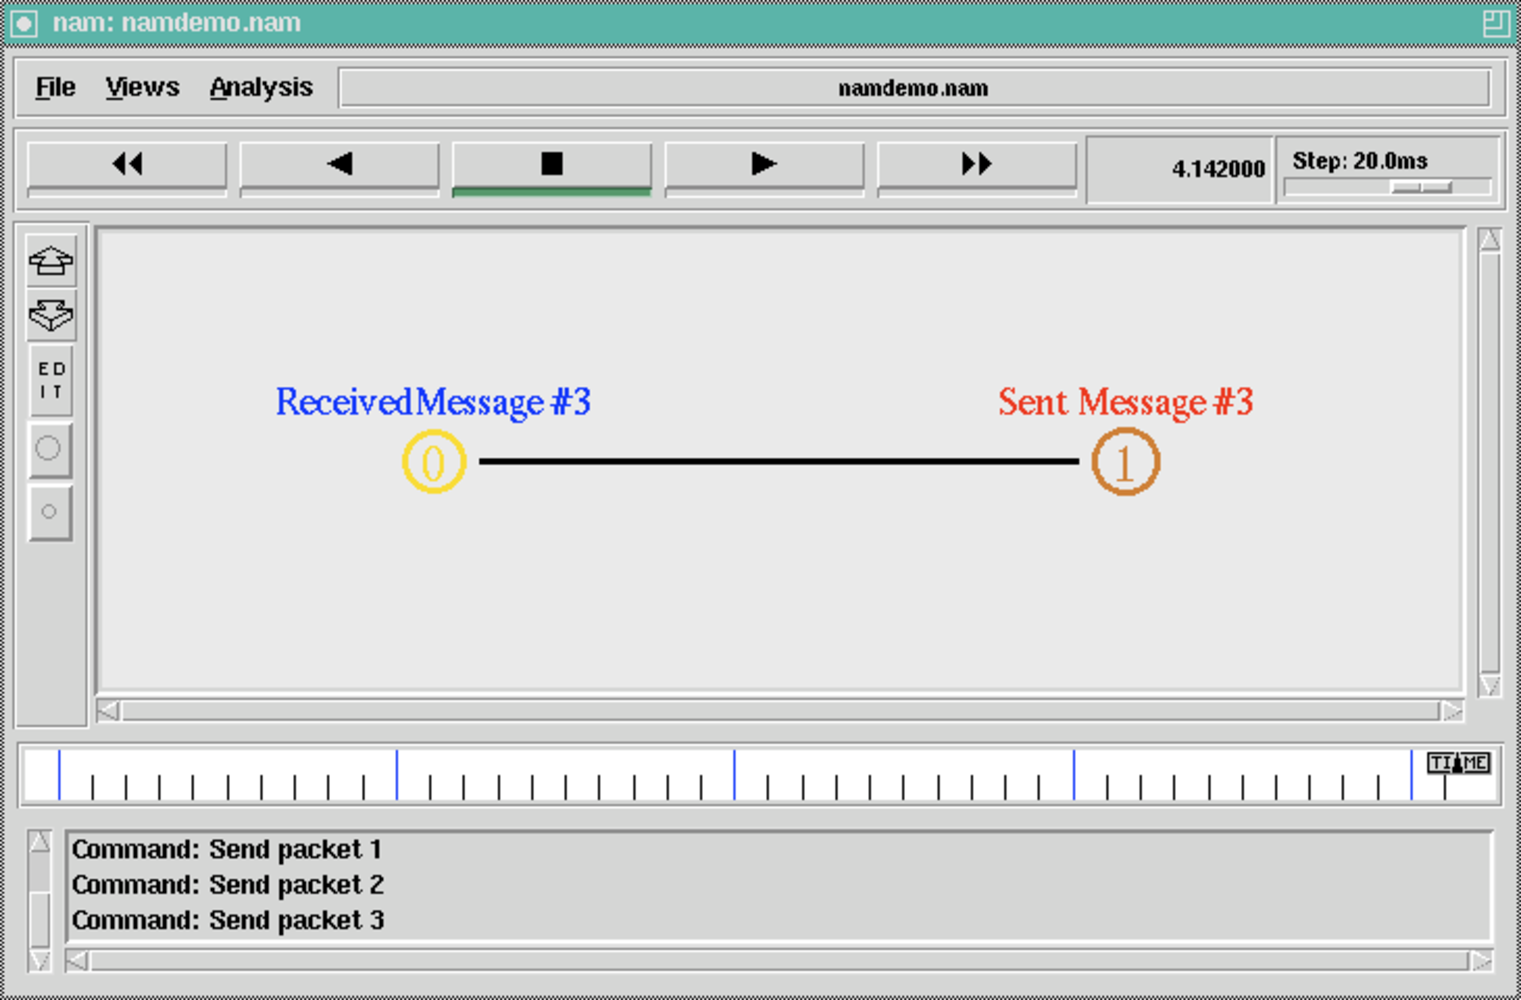
\includegraphics[scale=0.45]{images/namdemo}
\caption{The Output NAM display for the namdemo.tcl simulation}
\label{fig:namdemo}
\end{figure}
 
 \subsection{NAM Demo: The Java Side}
 \label{sec:nam:javaside}
 
 The demo actually demonstrates how to color nodes and add labels during a simulation. We use a simple multicast demo to ilustrate this. Every time a message is sent it is added as a label to the NAM animation and colors are changed. The commands are shown in the \emph{send} and \emph{receive} methods below from the NAMDemo class:

 
 \footnotesize
 \begin{verbatim}
   NAMCommands nam;

    public NamDemo() {
        this.setJavaDebugLevel(Level.DEBUG);
        this.setNativeDebugLevel(AgentJDebugLevel.detail);
        nam = this.getNamCommands();
        nam.setAnimationRate(0.02);
    }
 \end{verbatim}
 \normalsize

\footnotesize
 \begin{verbatim}
   public void send() {
        nam.setNodeColor(NAMCommands.NamColor.chocolate);
        try {
            String msg = "Message #" + msgcount;
            ++msgcount;
            DatagramPacket hi = new DatagramPacket(msg.getBytes(),msg.length(), group);
            nam.setNodeLabel("Sent " + msg, NAMCommands.LabelPosition.down, 
            							NAMCommands.NamColor.red);
            s.send(hi);
        } catch (IOException e) {
            e.printStackTrace();  
        }
    } 
 \end{verbatim}
 \normalsize

\footnotesize
 \begin{verbatim}
    public void receive() {
        nam.setNodeColor(NAMCommands.NamColor.gold);
        byte[] buf = new byte[1000];
        DatagramPacket recv = new DatagramPacket(buf, buf.length);
        try {
            s.receive(recv);
            String msg = new String(recv.getData());
            nam.setNodeLabel("Received" + msg, NAMCommands.LabelPosition.up, 
            						NAMCommands.NamColor.blue);
        } catch (IOException e) {
            e.printStackTrace(); 
        }
    }
 \end{verbatim}
 \normalsize
 
 \footnotesize
 \begin{verbatim}
 if (command.equals("send")) {
     nam.traceAnnotate("Command: Send packet " + msgcount);
     send();
 \end{verbatim}
 \normalsize


%\section{P2PS Demos}
%\label{sec:p2psdemos}

%\index{AgentJ P2PS Demonstrations}
%\index{AgentJ Peer-to-Peer Demonstrations}

%P2PS (Peer-to-Peer Simplified) \cite{p2ps} is a lightweight peer-to-peer 
%infrastructure. As the name suggests, P2PS aims to provide a simple 
%collection of middleware that a develop can use to write peer-to-peer 
%style applications, hiding the complexity of other similar architectures 
%such as JXTA~\cite{jxta} and JINI~\cite{jini2}.

%\index{JNI}

%Briefly, the P2PS infrastructure is based on XML based discovery and 
%communication, which makes it independent of any implementation 
%language and computing hardware. P2PS implementations could exist
%in any language and there is a specification which can be used to
%implement such, although at this time we have only built a prototype
%Java implementation. Furthermore, communication within P2PS is 
%not tied to any single transport protocol, such as TCP/IP, and 
%can be extended to include new protocols, such as Bluetooth or
%extend existing ones by writing new endpoint resolvers.  P2PS has 
%been designed to operate in highly dynamic, transient 
%environments and provides an overlay for discovering anything that
%a peer wants to advertise e.g. specific services, rendezvous (caching) peers,
%endpoint protocols etc.  P2PS dynamically discovers the capabilities of
%other peers at run-time and can negotiate and match how it 
%communicates and how it organises its peers.  This makes P2PS
%highly suitable for testing out different discovery mechanisms
%for two key reasons.  First, we can test the discovery mechanisms 
%built into P2PS (Multicast and Unicast) and secondly, we can easily
%extend this to include other protocols by writing new endpoint 
%resolvers. Thus, it provides a core extensible framework for testing 
%and exploring a number of mechanisms both within a simulated 
%environment or within a real-world application.

%\subsection{Simple P2PS Demos}

%This directory contains simulations using P2PS.  This work is on-going and 
%experimental, so run at your own risk :)

%\begin{enumerate}
%\item SimpleP2PS --- creates a direct UDP connection between two P2PS nodes
%\item P2PSComplex --- implements two nodes and uses multicast for discovery. Once discovered, P2PS figures out which protocols each have and negotiates a connection between them.  they connect and communicate a message.

%\end{enumerate}

%\subsection{Advanced P2PS Demos}

%These following demos use more complex network configurations and use a combination of discovery mechanisms for discovery of the nodes within the network. The network configuration consists of a client and server at the far side of the network and either zero, one, two or three rendezvous nodes in between them to aid in the discovery process. The demos use unicast or multicast depending on the mode.  Below is a brief summary of the demos:

%\begin{enumerate}
%\item P2PSMulticastDiscovery - multicast discovery demo using rendezvous nodes
%\item P2PSMulticastOneRendezvous - multicast discovery using one central independent rendezvous nodes
%\item P2PSUnicastDiscovery - unicast discovery using rendezvous nodes
%\item P2PSUnicastOneRendezvous - unicast discovery using one central independent rendezvous nodes
%\item P2PSUnicastTwoRendezvous - client and server unicast discovery using a cluster of three connected two rendezvous nodes
%\item P2PSUnicastThreeRendezvous - client and server unicast discovery using a cluster of three connected rendezvous nodes
%\end{enumerate}

%\begin{figure}
%\centering
%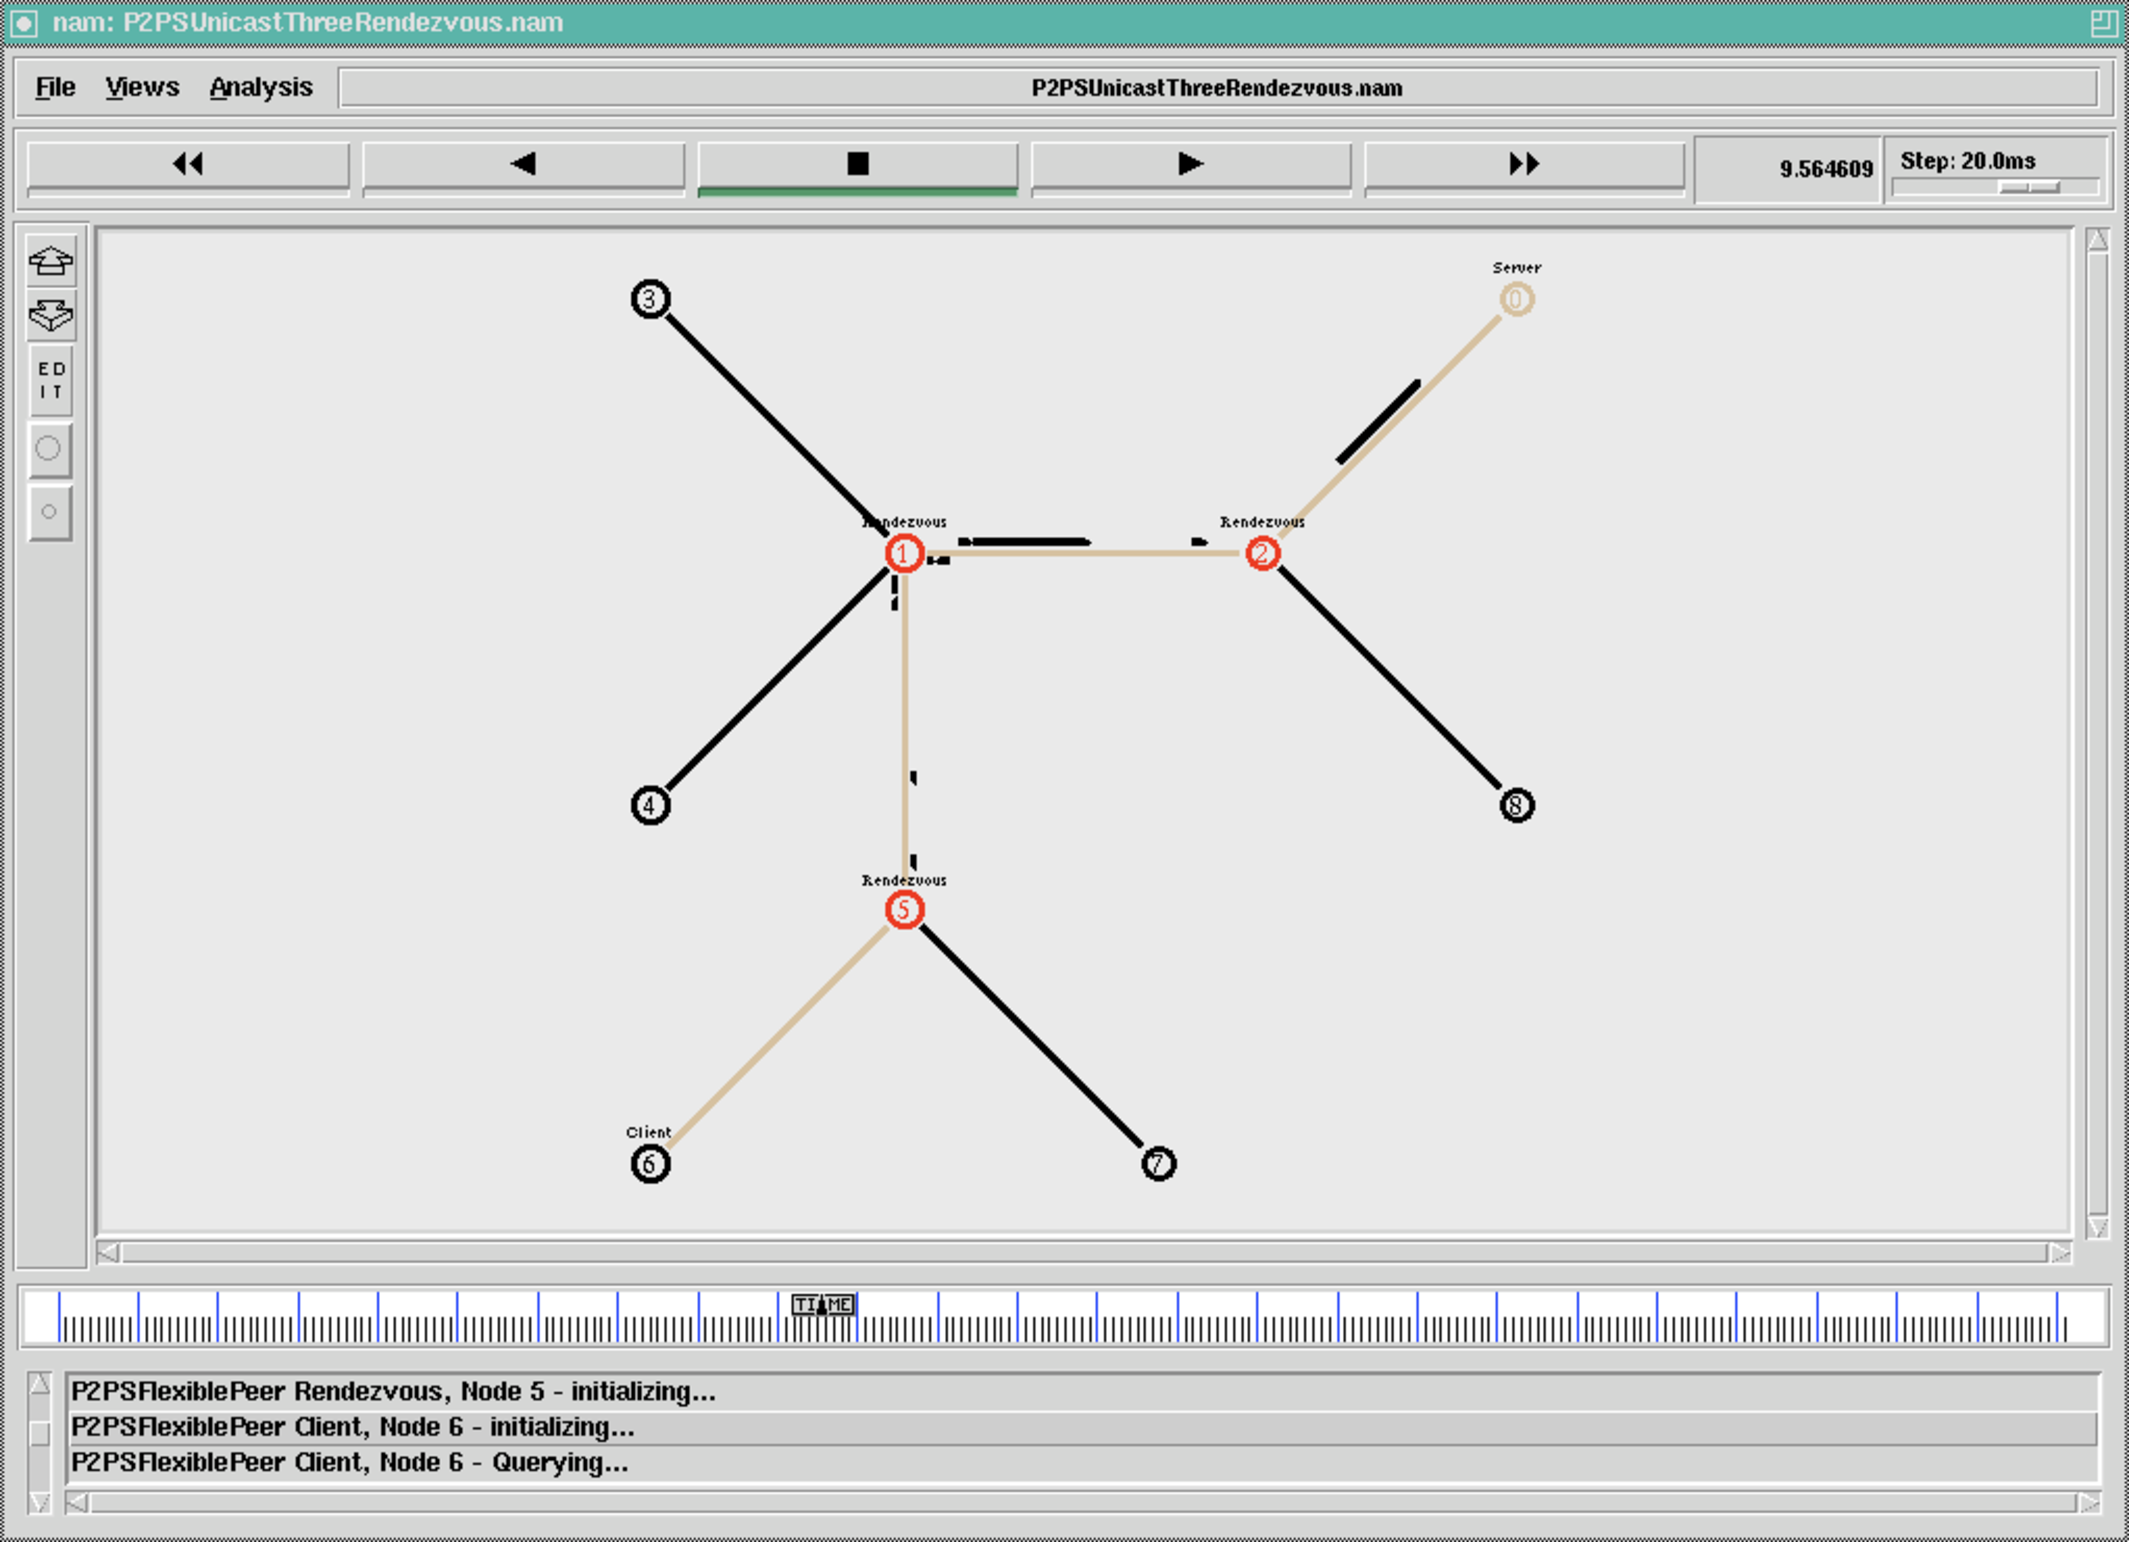
\includegraphics[scale=0.35]{images/p2psdemo}
%\caption{The network configuration for the Unicast Three Rendezvous P2PS demo.}
%\label{fig:p2psdemo}
%\end{figure}

%Figure \ref{fig:p2psdemo} shows a snapshot of a P2PS simulation.  In this example, there are three rendezvous peers in the center of the network, which are accessed by the client and server on the far sides.  The black segments show the data flow between the nodes during this time-slice of this simulation, and their length indicates the size of that data packet.  \noindent Go ahead and try these out yourself, you can find them in \emph{src/java/agentj/examples/p2ps}.



\footnotesize

\bibliographystyle{unsrt}
\bibliography{agentj}

\printindex

%%%%%%%%%%%%%%%%%%%%%%%%%%%%%%%%%%%%%%%%%%%%%%%%%%%%%%%%%%%%%%%%%%%%%%

\end{document}
